\documentclass[11pt,a4paper]{article}

\usepackage[utf8]{inputenc}
\usepackage[T1]{fontenc}
\usepackage[spanish,es-tabla]{babel}
\usepackage{microtype}
\usepackage[a4paper,margin=2.3cm,headheight=14pt]{geometry}
\usepackage{booktabs}
\usepackage{array}
\usepackage{tabularx}
\usepackage{multirow}
\usepackage{amsmath,amssymb,amsthm}
\usepackage{graphicx}
\usepackage{subcaption}
\usepackage{xcolor}
\usepackage{hyperref}
\hypersetup{colorlinks=true, linkcolor=black!75,
            urlcolor=blue!70!black, citecolor=accent}
\usepackage{enumitem}
\setlist{nosep, leftmargin=1.4em}
\usepackage{caption}
\captionsetup{font=small, labelfont=bf, labelsep=period}
\usepackage{fancyhdr}
\usepackage{titlesec}
\usepackage{footmisc}
\usepackage{siunitx}
\sisetup{group-separator={\,}, group-minimum-digits=4}

\definecolor{accent}{HTML}{1F4E79}
\definecolor{accent2}{HTML}{D26F3D}
\definecolor{good}{HTML}{2e8b57}
\definecolor{bad}{HTML}{d63a3a}

\titleformat{\section}{\large\bfseries\color{accent}}{\thesection}{0.6em}{}
\titleformat{\subsection}{\normalsize\bfseries\color{accent}}{\thesubsection}{0.6em}{}
\titleformat{\subsubsection}{\normalsize\bfseries\color{black!70}}{\thesubsubsection}{0.5em}{}

\pagestyle{fancy}
\fancyhf{}
\fancyhead[L]{\small\textit{UPV-EARTH $\times$ Planetary Boundaries -- AED completo}}
\fancyhead[R]{\small\thepage}
\renewcommand{\headrulewidth}{0.3pt}

\newcommand{\good}[1]{\textbf{\textcolor{accent}{#1}}}
\newcommand{\bad}[1]{\textbf{\textcolor{bad}{#1}}}
\newcommand{\pb}[1]{\textsc{pb#1}}

\title{\vspace*{-1.2cm}
\Large\bfseries\textcolor{accent}{Análisis Exploratorio de Datos y Clasificación Multilabel\\
del corpus científico UPV-EARTH en Planetary Boundaries}\\[0.4em]
\large\textit{Memoria técnica para revisión sénior}}
\author{\normalsize Equipo de Ciencia de Datos UPV-EARTH \\
\small \texttt{31\,560 abstracts (1980--2025) -- 9 Planetary Boundaries -- 6 modelos evaluados}}
\date{Mayo 2026}

\begin{document}
\maketitle
\thispagestyle{empty}
\vspace*{-1em}

\begin{abstract}
\noindent
Presentamos un Análisis Exploratorio de Datos (AED) y un estudio de clasificación multilabel sobre el corpus científico UPV-EARTH (\num{31560} abstracts, 1980--2025) en el marco de las nueve \emph{Planetary Boundaries} (PB) \cite{steffen2015planetary,rockstrom2009safe}. El AED se estructura en siete bloques: trazabilidad del corpus, definición operativa de los PBs, perfil PB global (la ``firma'' UPV), evolución temporal, estructura sistémica (coocurrencias y red), estructura semántica (UMAP, clustering, Sankey topics-PB) y comportamiento de modelos. Se evalúan seis enfoques zero-shot/few-shot (léxico, TF-IDF, BERT-base, RoBERTa, SciBERT, SPECTER) contra un ground truth humano de 98 papers con 130 PBs anotados, mediante un panel de siete métricas y dos fórmulas compuestas: una de éxito ponderado y un Mean Reciprocal Rank ponderado por nivel de anotación. \textbf{El hallazgo principal} es que TF-IDF con threshold recalibrado supera consistentemente a los transformers \emph{no fine-tuneados} en todas las métricas: F1 multilabel $= 0{,}61$, score MRR ponderado $= 0{,}77$, y recuperación del PB principal en top-2 = 77\,\%. La firma PB de la UPV se concentra en \pb1, \pb2 y \pb6 ($\approx 60\,\%$ del corpus PB-related), con un vacío estructural en \pb8 (2\,\%) y una débil presencia en \pb5 (6\,\%), inconsistente con el perfil tecnológico esperable de una universidad mediterránea. La estructura sistémica (coocurrencias \pb3$\leftrightarrow$\pb9, \pb4$\leftrightarrow$\pb5, \pb6$\leftrightarrow$\pb7) emerge limpiamente en todos los modelos competitivos, validando el etiquetado a posteriori. Discutimos limitaciones metodológicas relevantes (n=98, leak de threshold, anotador único) y proponemos una receta de ensemble por clase y un protocolo de fine-tune contrastivo de SPECTER como siguiente paso crítico.
\end{abstract}

\medskip
\noindent\textbf{Palabras clave:} planetary boundaries; clasificación multilabel; representación documental; SPECTER; embeddings semánticos; cienciometría; perfil temático institucional.

\tableofcontents
\clearpage

% ============================================================
\section{Introducción}

\subsection{Contexto y motivación}

El marco \emph{Planetary Boundaries} \cite{steffen2015planetary} establece nueve sistemas terrestres cuya estabilidad es condición necesaria para un Holoceno operativo. Caracterizar qué fracción de la producción científica de una institución contribuye a la comprensión, mitigación o monitorización de cada PB es una pregunta cienciométrica de creciente interés \cite{larosa2023climate,upv_ods_2024}. La Universitat Politècnica de València (UPV) acumula varias décadas de producción científica relacionada con \emph{earth science}, ingeniería ambiental, agronomía y química, lo que la hace candidata natural para este análisis.

La pregunta operativa es directa: dado un abstract de un paper UPV, ¿a qué Planetary Boundary(es) pertenece su tema? La complicación es que el problema tiene \textbf{multilabel}: un mismo paper puede contribuir a varias PBs simultáneamente, y los PBs no son ortogonales (e.g.\ \pb6 y \pb7 comparten un solapamiento físico amplio).

\subsection{Naturaleza del problema y posicionamiento metodológico}

Disponemos de \num{31560} abstracts en el corpus pero solo \textbf{138 anotaciones manuales} con etiqueta PB. La consecuencia metodológica es importante:

\begin{itemize}
\item No es viable un entrenamiento supervisado al uso. La mediana de soporte por clase ronda los 8 documentos. Cualquier modelo entrenado supervisadamente sufrirá overfit catastrófico y producirá estimaciones inestables.
\item La aproximación correcta es \textbf{clasificación zero-shot/few-shot por similitud semántica}: cada PB se representa textualmente mediante una descripción operativa (definición, keywords, frases ejemplo, reglas de exclusión) y se compara contra cada abstract en un espacio de representación.
\item La elección del espacio de representación es lo que distingue a los seis modelos evaluados. Los baselines (léxico, TF-IDF) operan en espacios sparsos definidos por el vocabulario; los transformers operan en espacios densos pre-entrenados.
\end{itemize}

\subsection{Objetivos y estructura del documento}

\begin{enumerate}
\item Caracterizar el corpus y demostrar su calidad antes de derivar conclusiones (§\ref{sec:corpus}).
\item Construir y justificar la representación operativa de cada PB (§\ref{sec:pb_def}).
\item Determinar el perfil PB de la UPV: qué PBs dominan, cuáles son marginales (§\ref{sec:perfil}).
\item Estudiar la evolución temporal del perfil para distinguir crecimiento global vs cambio de agenda (§\ref{sec:temporal}).
\item Estudiar la estructura sistémica (coocurrencias, red PB) (§\ref{sec:sistemico}).
\item Estudiar la estructura semántica del corpus mediante embeddings y clustering (§\ref{sec:semantico}).
\item Evaluar críticamente seis modelos de clasificación frente a anotación humana, incluyendo métricas estándar y dos fórmulas compuestas (§\ref{sec:modelos}).
\item Discutir limitaciones, proponer recomendación operativa y siguientes pasos (§\ref{sec:discusion}).
\end{enumerate}

% ============================================================
\section{Corpus: trazabilidad, calidad y limpieza}\label{sec:corpus}

\subsection{Pipeline de construcción}

El corpus se construye a partir de descargas mixtas de Scopus y OpenAlex, deduplicadas por DOI y por hash de título+año, y filtradas por longitud, idioma y completitud. La trazabilidad completa se preserva en \texttt{master\_corpus\_mixto\_traceability.csv}, donde cada documento mantiene su \texttt{filter\_status} y \texttt{filter\_reason}. El flujo agregado es:

\[
\underbrace{\num{44970}}_{\text{raw}} \xrightarrow{\text{dedup}} \underbrace{\num{44593}}_{\text{dedup}} \xrightarrow{\text{filtros}} \underbrace{\num{31634}}_{\text{filtrados}} \xrightarrow{\text{limpieza inferencia}} \underbrace{\num{31560}}_{\text{usables}}
\]

Las pérdidas son atribuibles a: (i) duplicados por DOI o por título+año ($\sim$235), (ii) abstracts de longitud inferior a 500 caracteres ($\sim$\num{11744}, 26\,\%), (iii) idiomas no anglosajones ($\sim$300), y (iv) registros con \texttt{abstract\_norm} vacío ($\sim$377). La conservación del 69\,\% del corpus crudo es coherente con prácticas habituales en cienciometría sobre Scopus/OpenAlex \cite{upv_ods_2024}.

\subsection{Limpieza defensiva para inferencia}\label{sec:limpieza}

Antes de pasar los abstracts por los modelos se aplica una función \texttt{clean\_for\_inference} que elimina contaminantes capaces de consumir tokens útiles del \texttt{max\_length=256}: URLs, emails, etiquetas HTML, entidades HTML, DOIs, boilerplate de copyright editorial (Elsevier, Wiley, MDPI, Springer, Taylor \& Francis), caracteres de control y normalización de espacios. Adicionalmente se descartan abstracts $<200$ caracteres tras limpiar. La pérdida adicional es de 75 documentos (0{,}24\,\%), lo que confirma que el filtrado upstream era ya bastante estricto.

\subsection{Calidad textual y metadata}

La Figura~\ref{fig:corpus} resume cinco facetas del corpus: pipeline, evolución temporal, distribución de longitud de abstract, completitud de metadatos y fuentes.

\begin{figure}[h]
\centering
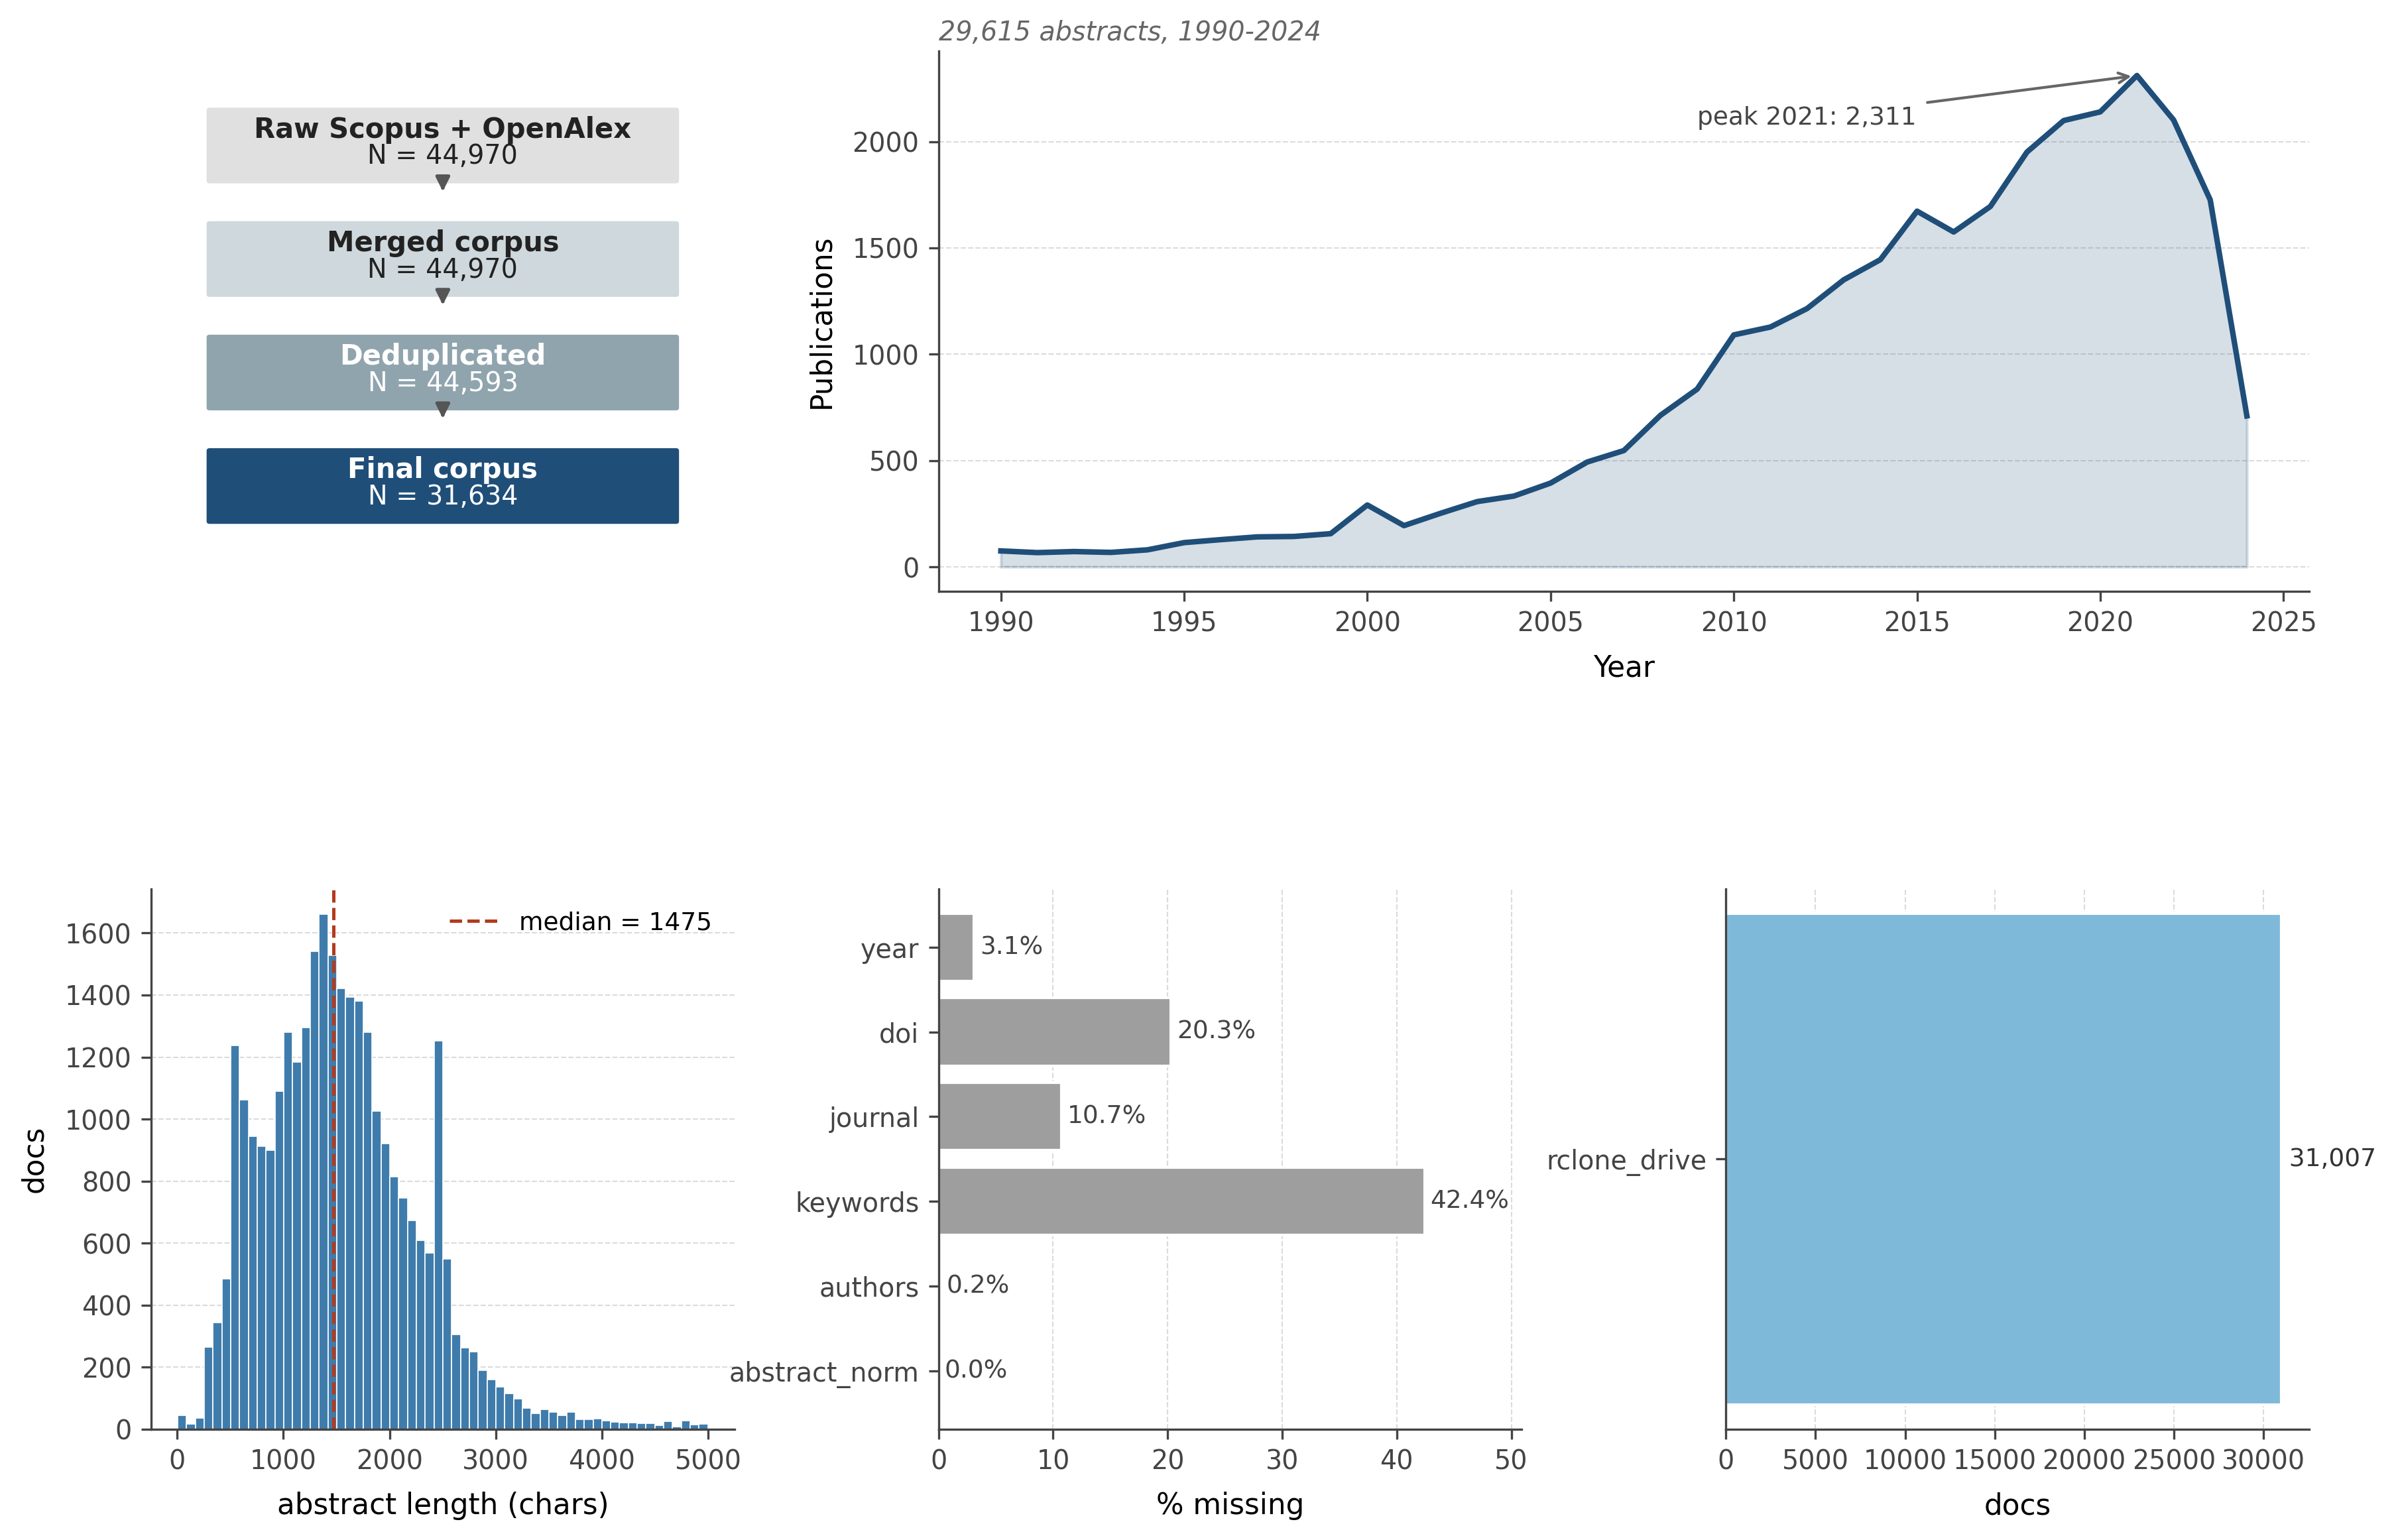
\includegraphics[width=\linewidth]{figures/01_corpus_overview.png}
\caption{Panel de calidad del corpus. \textbf{(a)} Pipeline con números absolutos. \textbf{(b)} Evolución temporal de publicaciones (pico en 2021 con \num{2311} publicaciones; caída 2022--2024 es artefacto de cobertura Scopus/OpenAlex, no productividad). \textbf{(c)} Longitud de abstracts log-normal, mediana \num{1475} caracteres. \textbf{(d)} Completitud: \texttt{keywords} 42\,\% null, \texttt{doi} 20\,\%. \textbf{(e)} Fuente consolidada upstream.}
\label{fig:corpus}
\end{figure}

\textbf{Implicaciones para el AED:} la alta proporción de \texttt{keywords} nulas (42\,\%) impide análisis basados en keywords del autor; obliga a leer semánticamente el contenido. La fracción de DOIs nulos (20\,\%) afecta a la trazabilidad bibliográfica pero no a la inferencia. La caída temporal 2022--2024 obliga a usar series normalizadas (\% del año) para análisis longitudinales, no absolutas.

% ============================================================
\section{Definición operativa de los Planetary Boundaries}\label{sec:pb_def}

Los PBs se representan en \texttt{pb\_reference.csv} mediante un esquema relacional compuesto por: \texttt{pb\_code}, \texttt{aliases}, \texttt{short\_definition}, \texttt{long\_definition}, \texttt{control\_variables}, \texttt{core\_keywords}, \texttt{extended\_keywords}, \texttt{applied\_keywords\_upv}, \texttt{method\_keywords\_contextual}, \texttt{sector\_keywords}, \texttt{example\_phrases}, \texttt{activation\_logic} y \texttt{exclusion\_notes}. A partir de este esquema se deriva un \emph{documento textual} por PB (\texttt{pb\_corpus\_documents.csv}) que combina definición, keywords y frases en un texto único que actúa de \emph{anchor} para la similitud.

\begin{table}[h]
\centering\small
\begin{tabular}{l l p{6.8cm}}
\toprule
\textbf{PB} & \textbf{Nombre} & \textbf{Núcleo conceptual (\texttt{core\_keywords} resumidas)} \\
\midrule
\pb1 & Climate Change & greenhouse gases, radiative forcing, climate sensitivity, mitigation, adaptation \\
\pb2 & Ocean Acidification & aragonite, carbonate chemistry, $p$CO$_2$, ocean pH \\
\pb3 & Stratospheric Ozone & ozone depletion, CFCs, polar vortex, halogens \\
\pb4 & Biogeochemical Flows & nitrogen cycle, phosphorus loading, eutrophication \\
\pb5 & Freshwater Use & blue water, groundwater, water scarcity, hydrology \\
\pb6 & Land-System Change & deforestation, land cover change, urban expansion \\
\pb7 & Biosphere Integrity & biodiversity, ecosystem function, BII, genetic diversity \\
\pb8 & Novel Entities & microplastics, EDCs, nanomaterials, pollutants \\
\pb9 & Atmospheric Aerosol & aerosol optical depth, particulate matter, AOD \\
\bottomrule
\end{tabular}
\caption{Núcleo conceptual de los nueve PBs. Las definiciones completas y reglas de exclusión están en \texttt{pb\_reference.csv}.}
\label{tab:pbs}
\end{table}

\paragraph{Familias temáticas.} Agrupamos los nueve PBs en tres familias para reducir dimensionalidad visual:
\begin{itemize}
\item \textbf{Atmosphere \& Climate}: \pb1, \pb2, \pb3, \pb9.
\item \textbf{Land, Water \& Biosphere}: \pb5, \pb6, \pb7.
\item \textbf{Chemical \& Biogeochemical Pressure}: \pb4, \pb8.
\end{itemize}
La agrupación tiene base física: PBs de la familia atmosférica comparten dinámica radiativa o de transporte; los de tierra/agua/biosfera tienen acoplamiento ecosistémico; los químicos representan presiones por aporte antropogénico de materiales.

% ============================================================
\section{Perfil PB de la UPV: la ``firma'' institucional}\label{sec:perfil}

\subsection{Distribución global}

Aplicando TF-IDF con threshold óptimo $\tau{=}0{,}03$, $\delta{=}0{,}08$ sobre los \num{31560} abstracts y expandiendo multilabel, se obtienen $\sim$\num{91000} asignaciones PB. La distribución agregada se muestra en la Figura~\ref{fig:perfil}.

\begin{figure}[h]
\centering
\begin{subfigure}{0.48\linewidth}
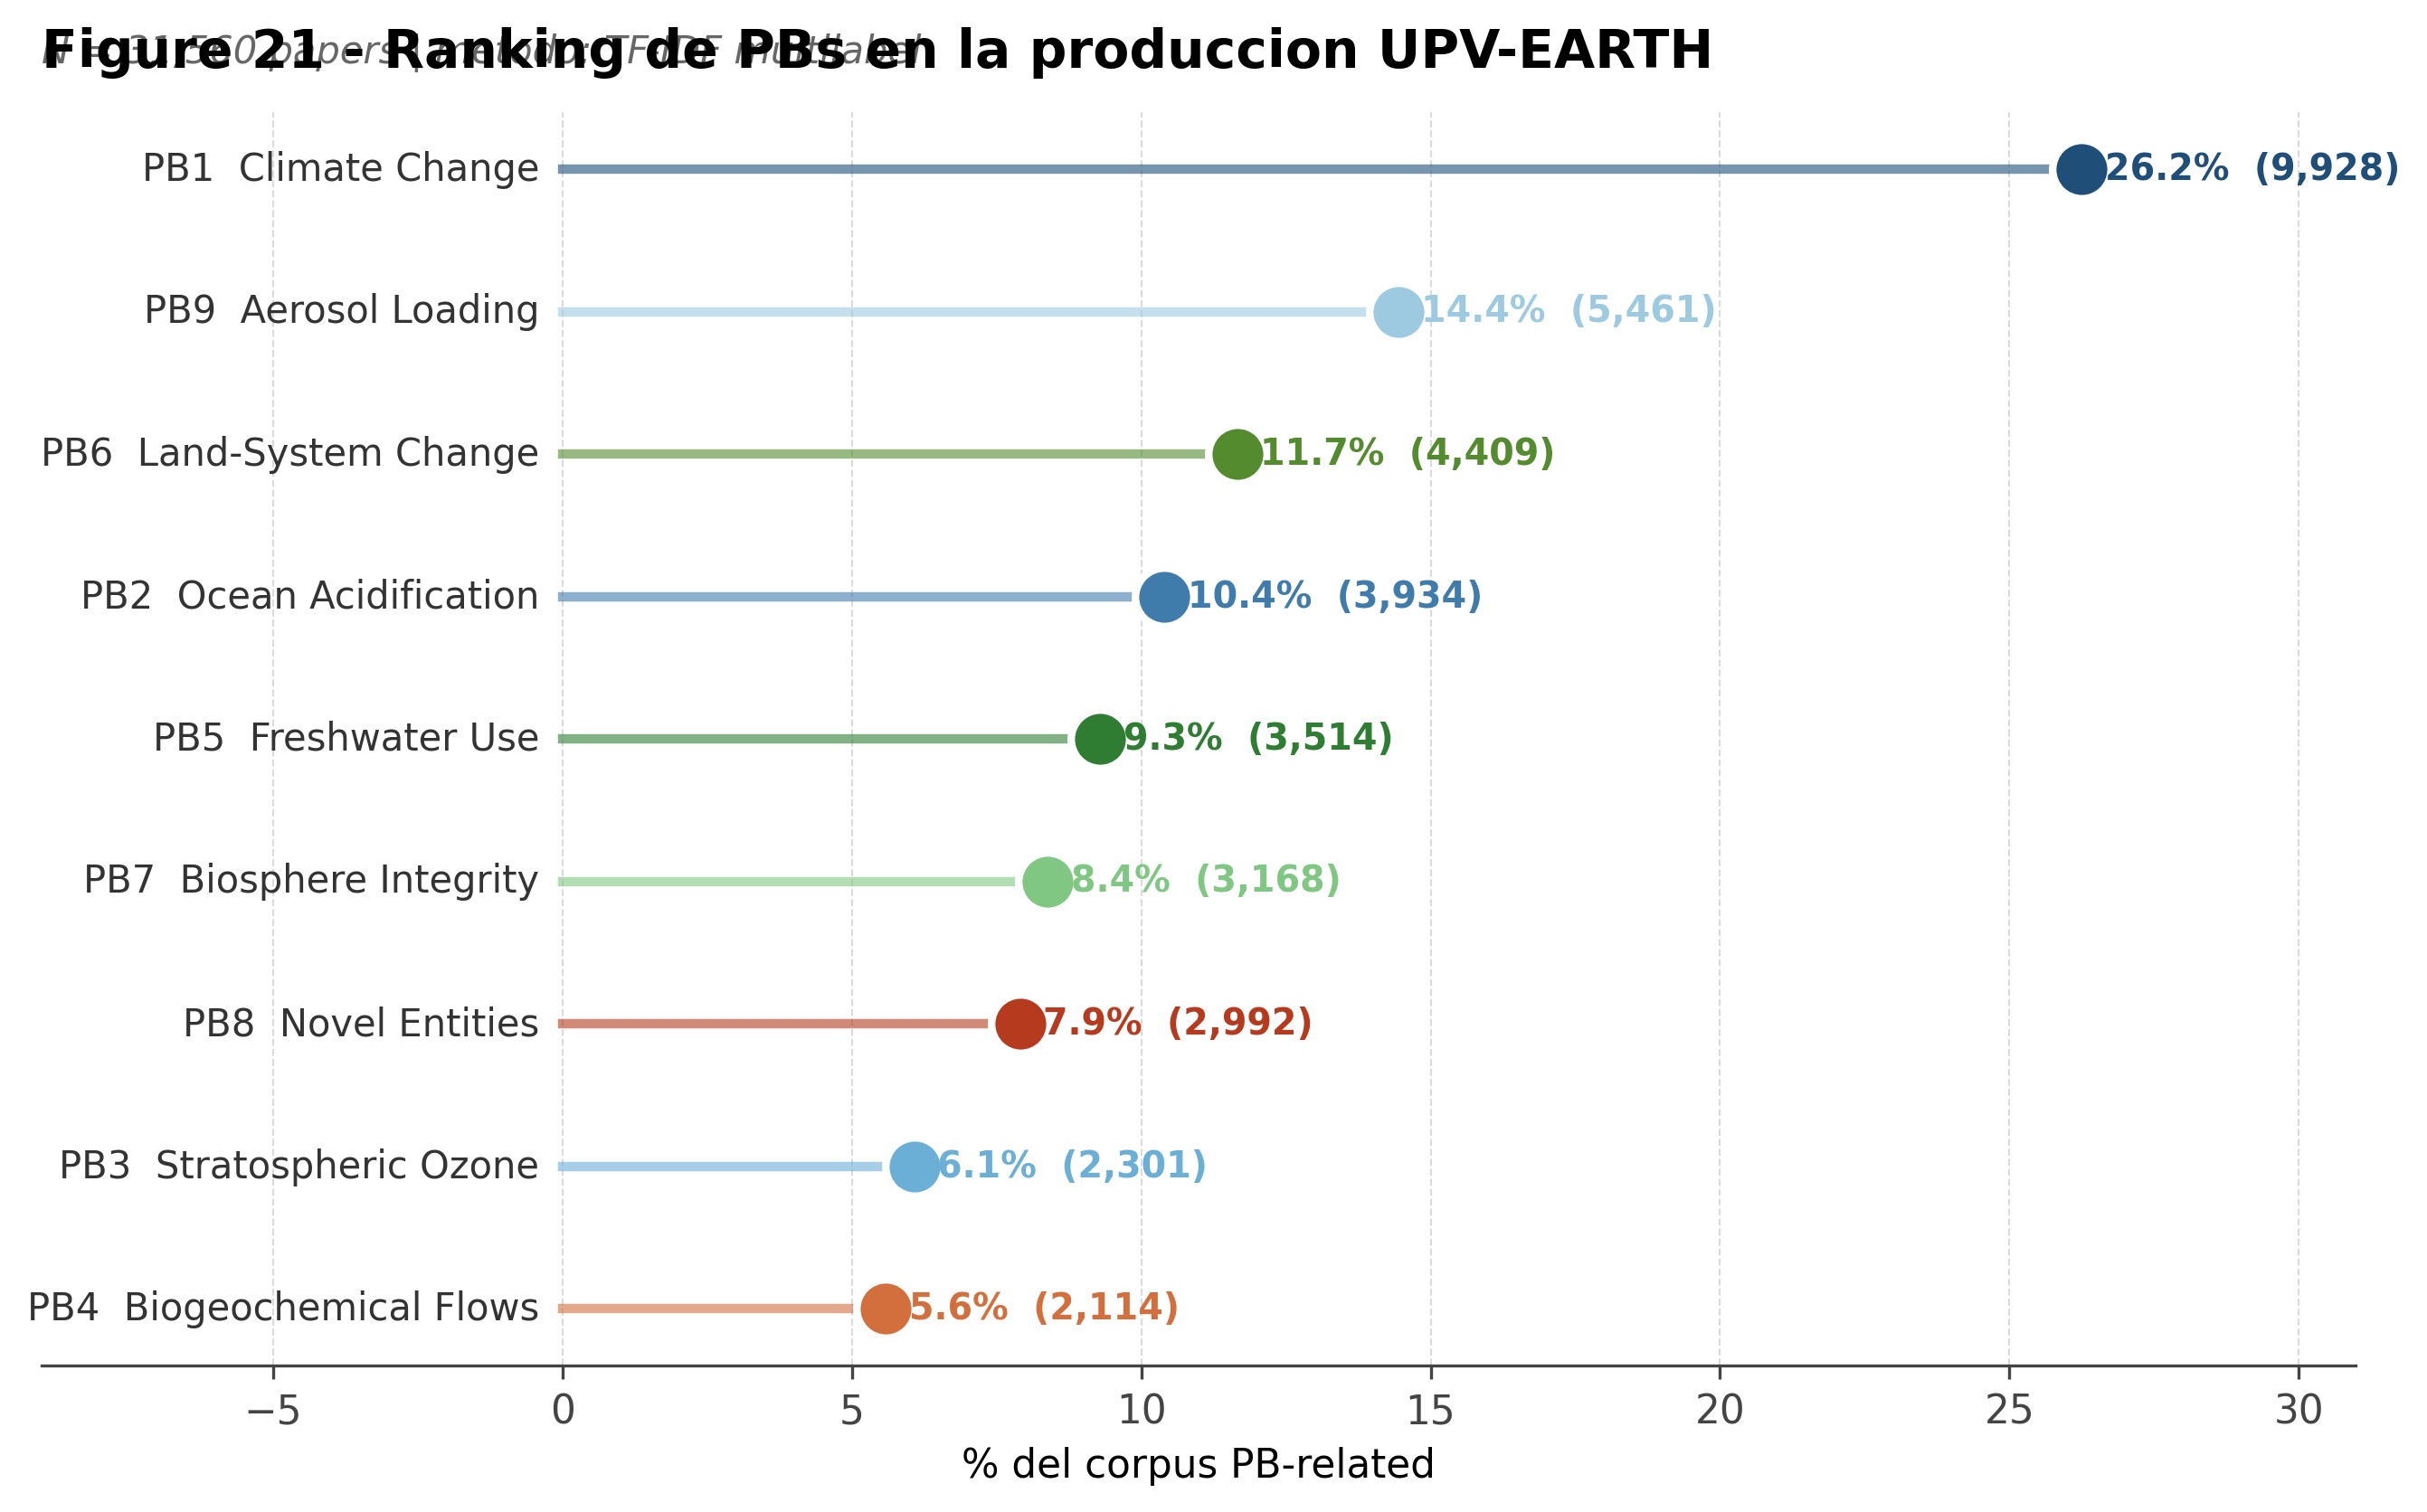
\includegraphics[width=\linewidth]{figures/21_lollipop_ranking.png}
\caption{Ranking tipo \emph{lollipop}.}
\end{subfigure}
\hfill
\begin{subfigure}{0.48\linewidth}
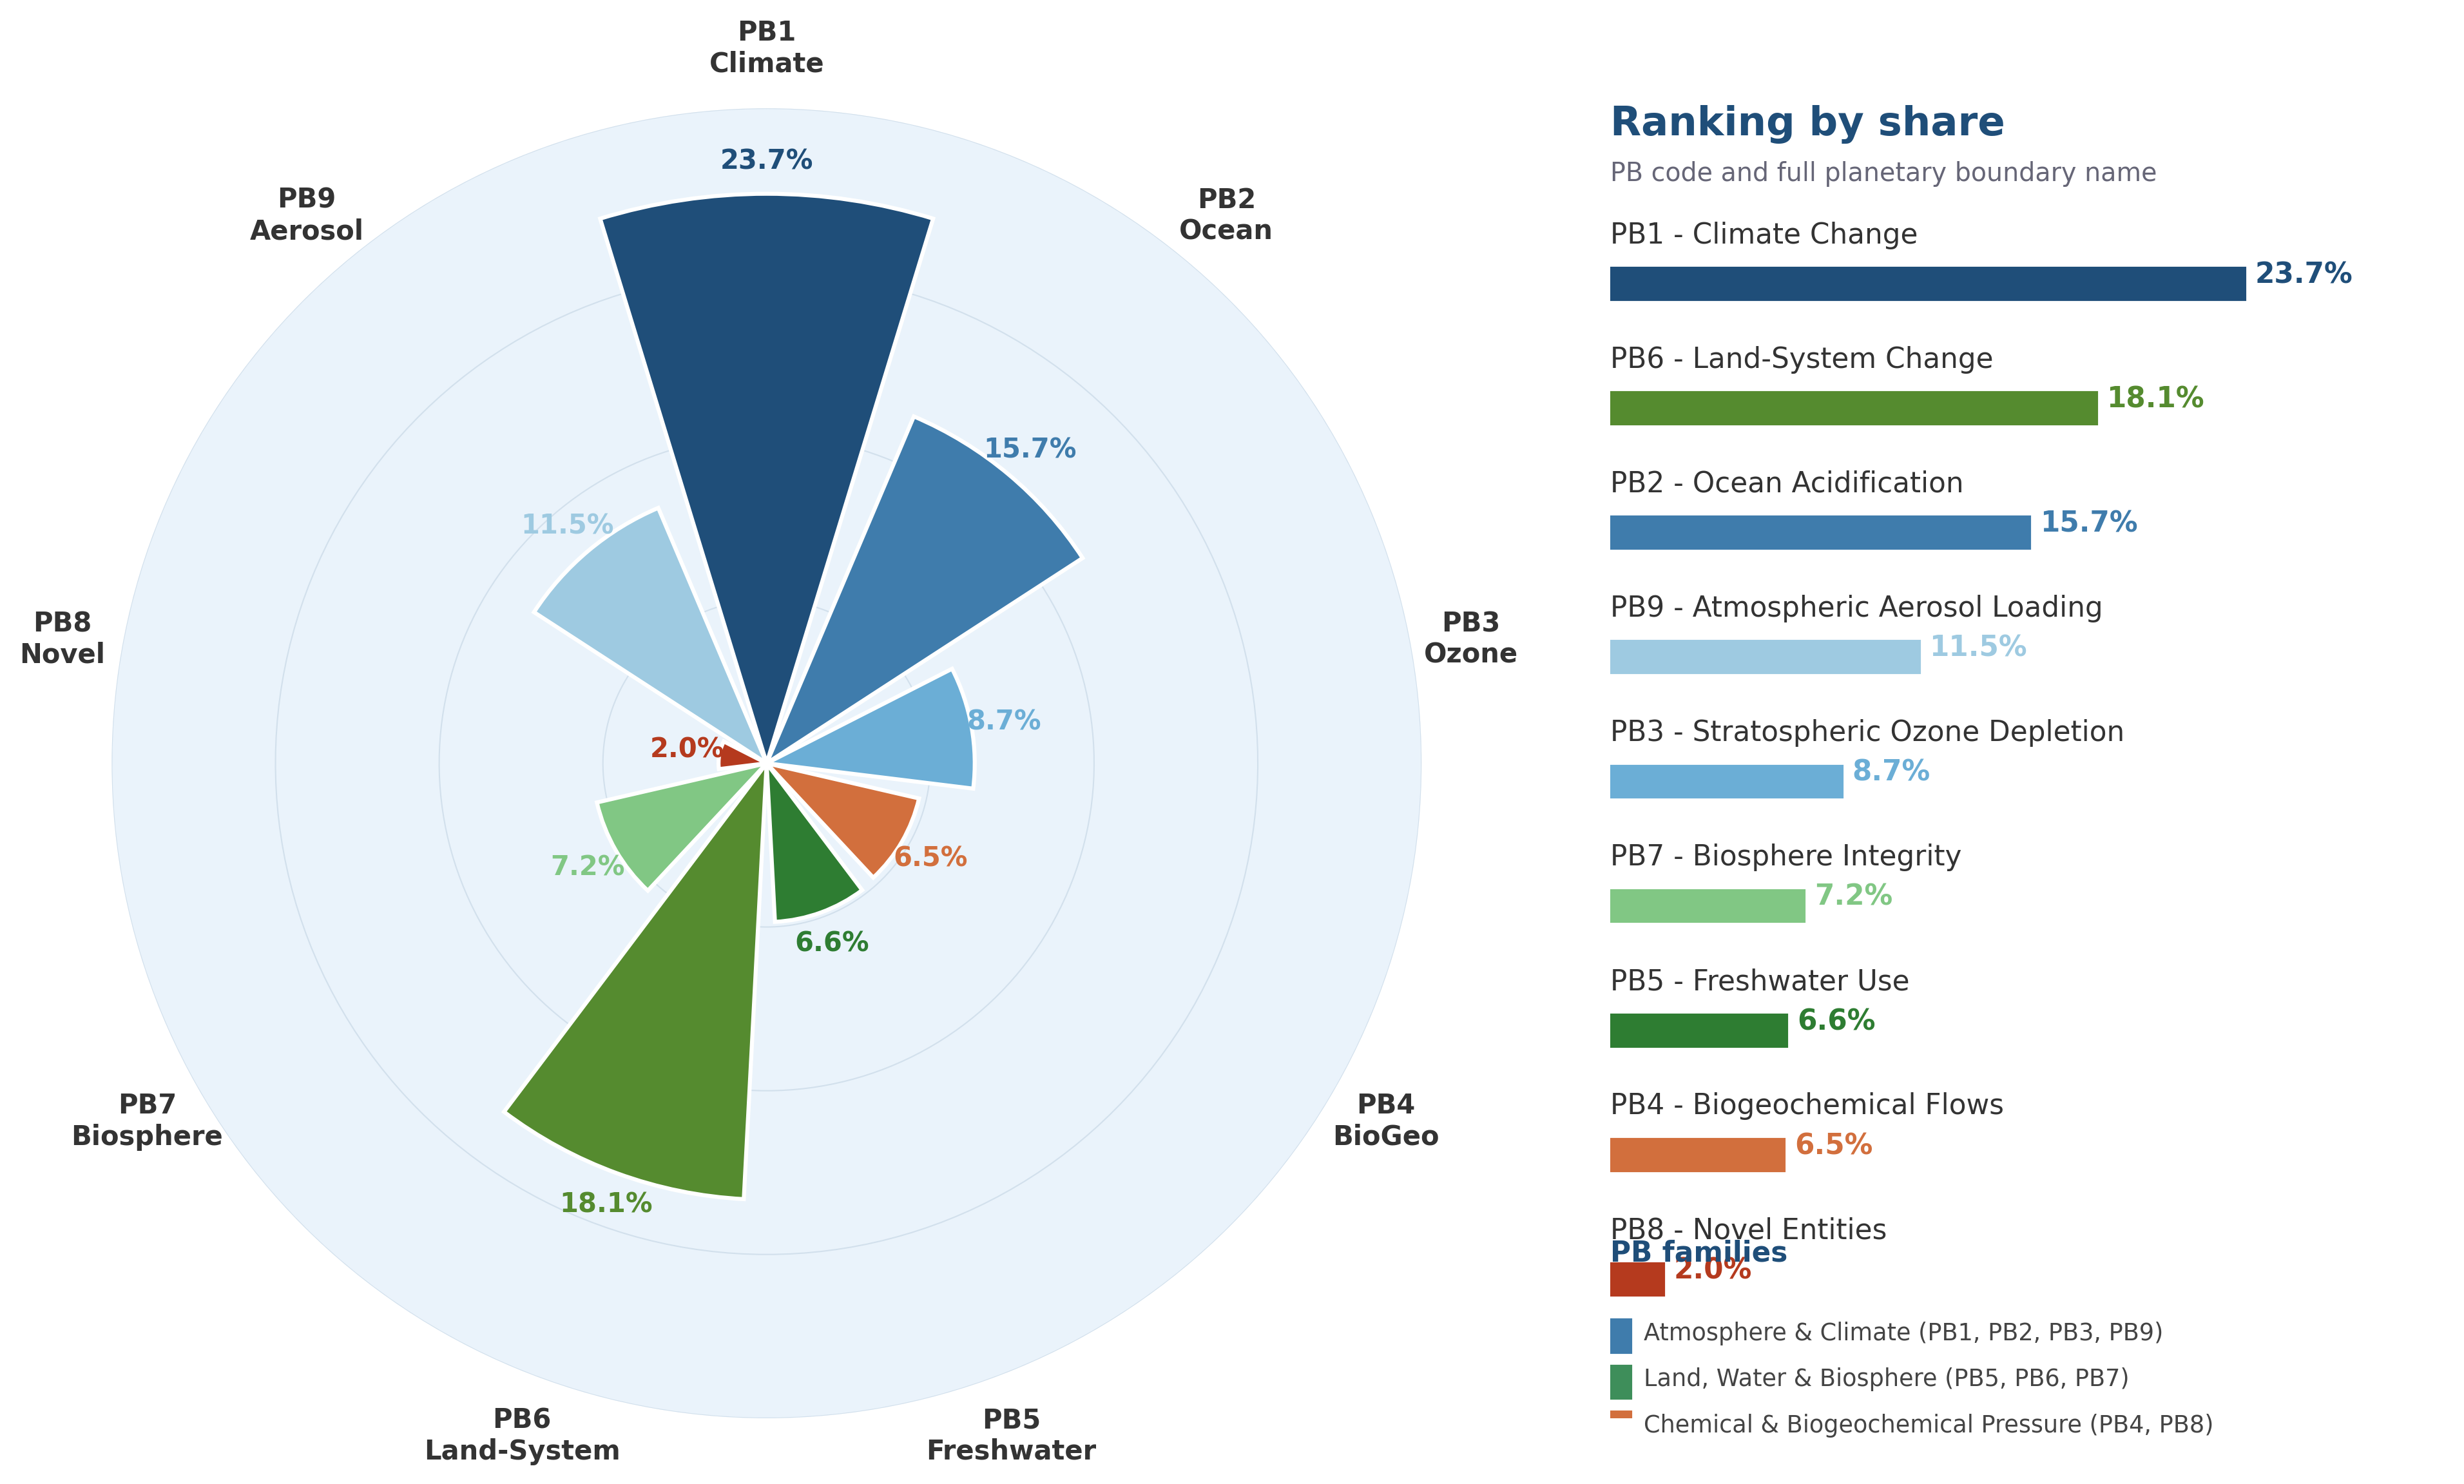
\includegraphics[width=\linewidth]{figures/02_pb_radial_signature.png}
\caption{Firma radial (perfil institucional).}
\end{subfigure}\\[0.6em]
\begin{subfigure}{\linewidth}
\centering
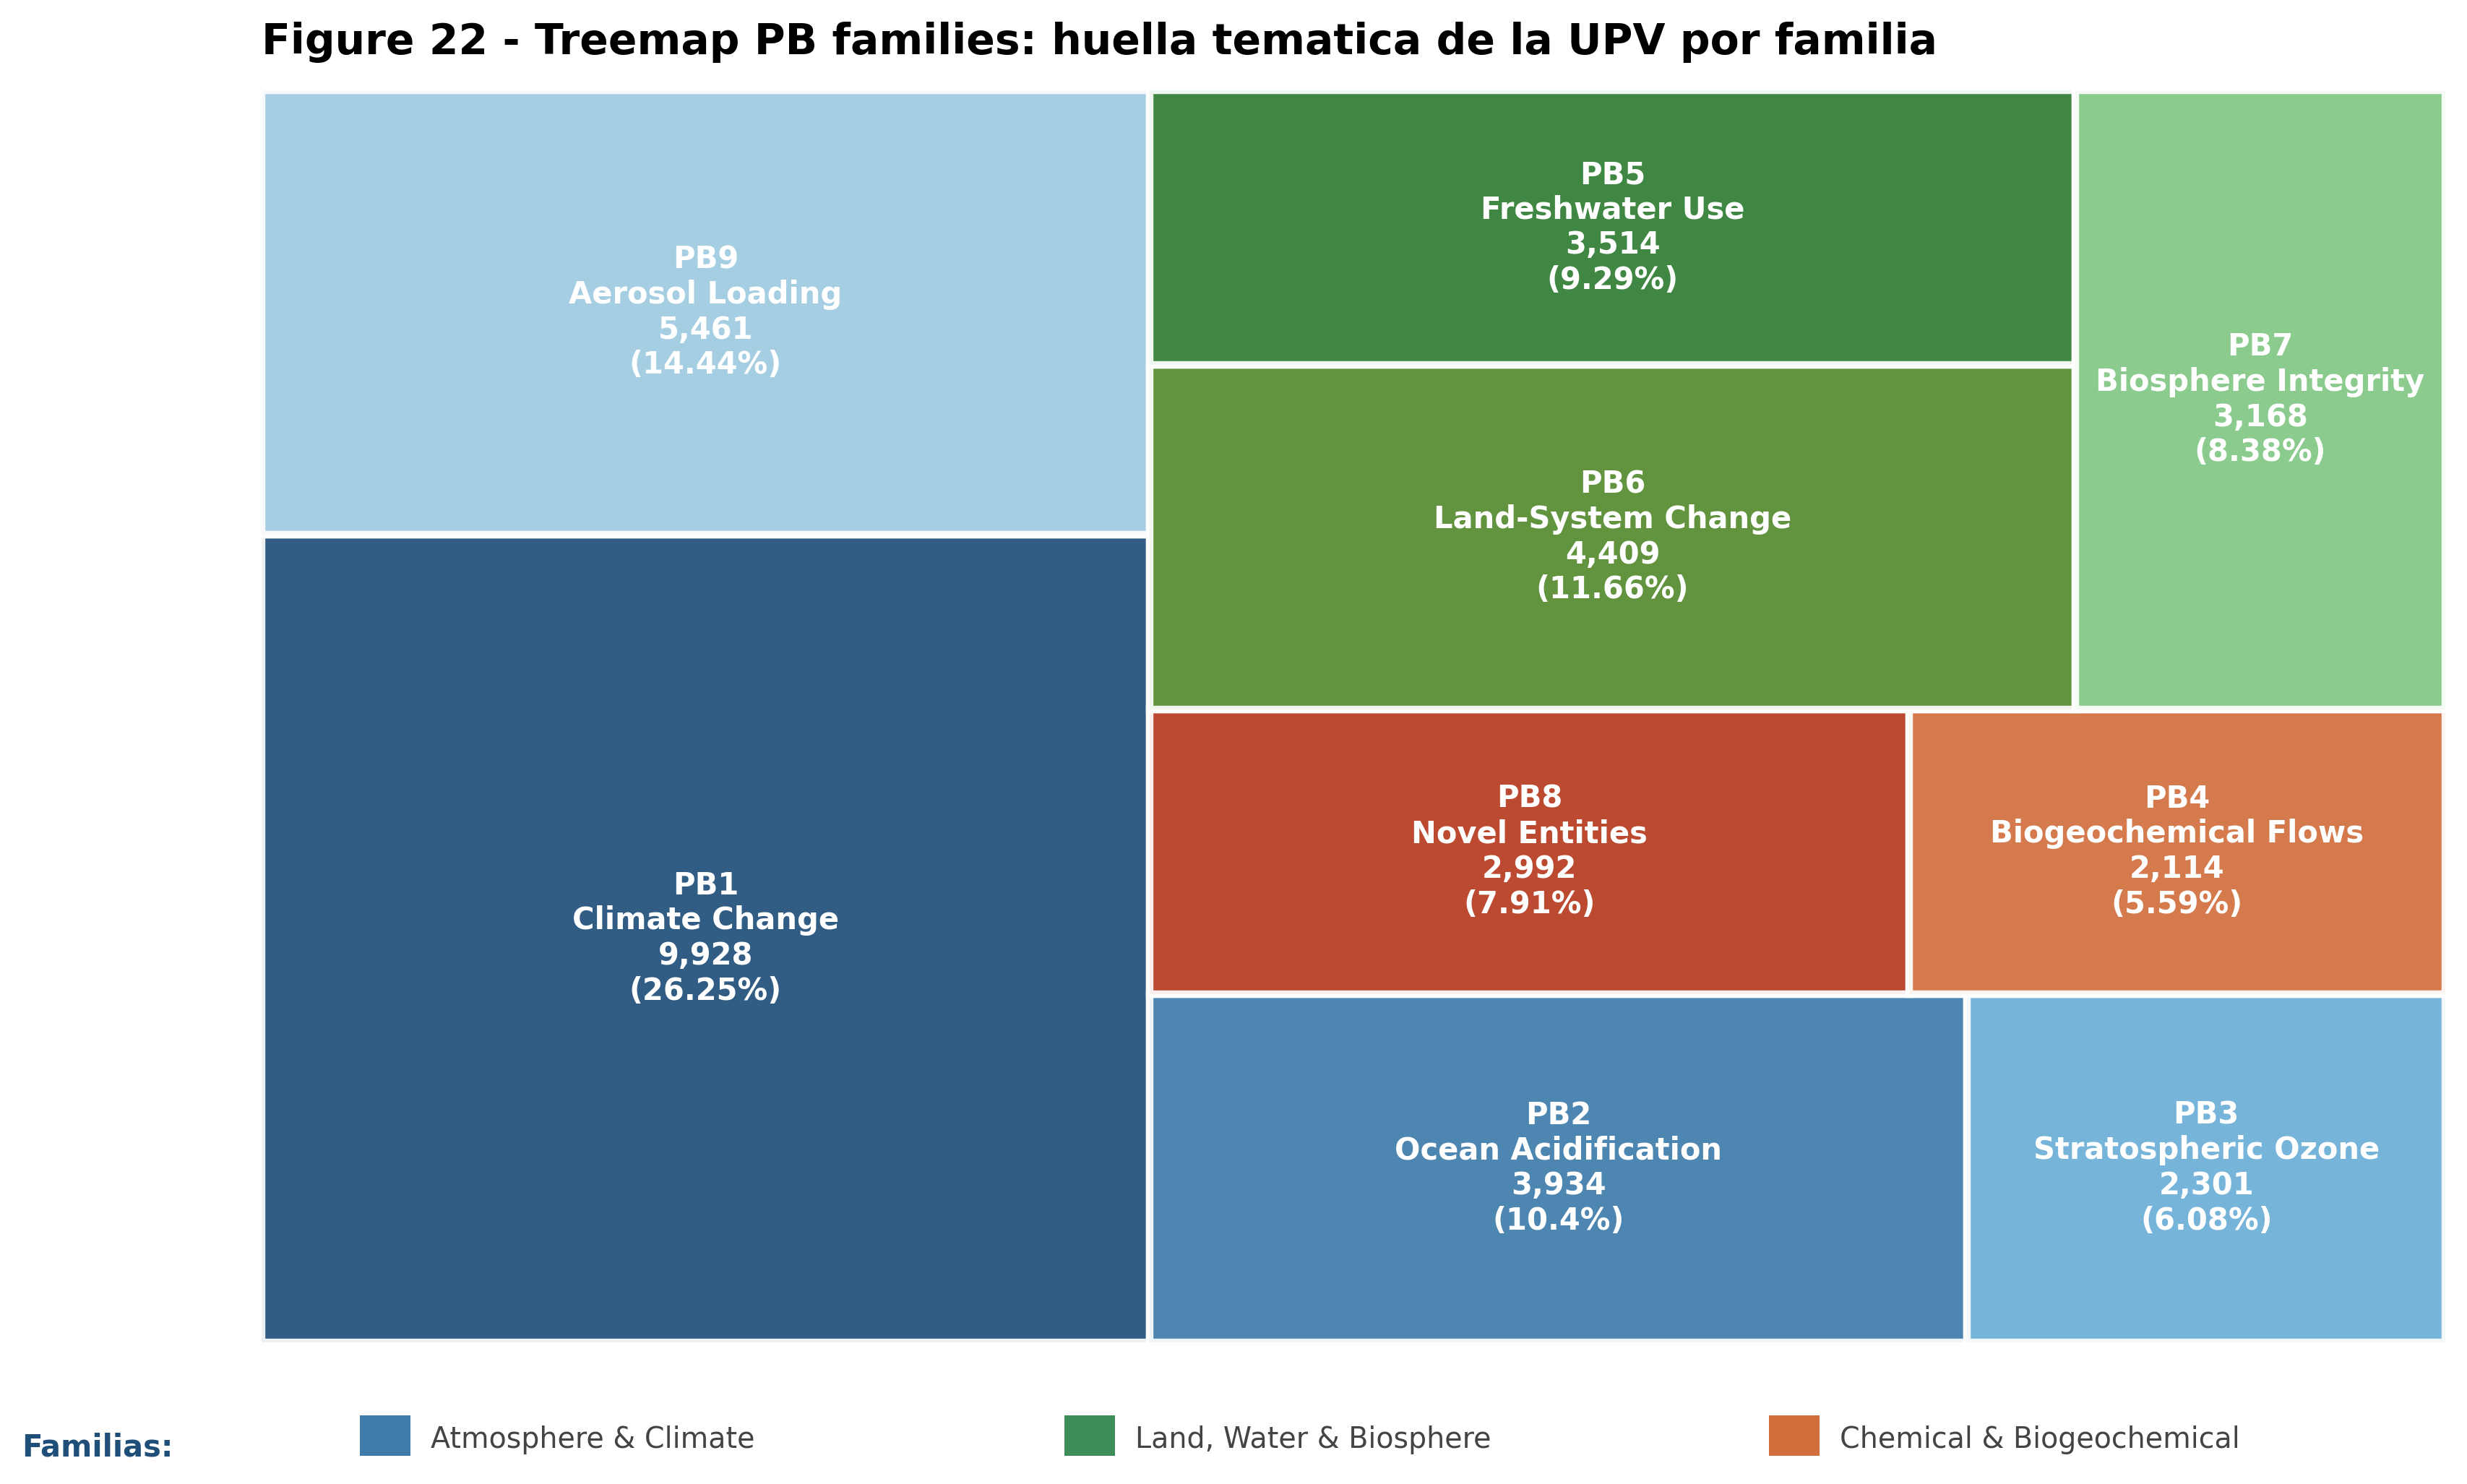
\includegraphics[width=0.85\linewidth]{figures/22_treemap_families.png}
\caption{Treemap por familias PB.}
\end{subfigure}
\caption{Perfil PB de la UPV. Tres lecturas complementarias del mismo fenómeno.}
\label{fig:perfil}
\end{figure}

\begin{table}[h]
\centering\small
\begin{tabular}{r l r r l}
\toprule
\textbf{Rank} & \textbf{PB} & \textbf{\# asignaciones} & \textbf{\% del corpus PB-related} & \textbf{Familia} \\
\midrule
1 & \good{\pb1 Climate Change} & \num{18139} & \good{23{,}7} & Atmosphere \& Climate \\
2 & \good{\pb6 Land-System Change} & \num{13927} & \good{18{,}1} & Land, Water \& Biosphere \\
3 & \good{\pb2 Ocean Acidification} & \num{12027} & 15{,}7 & Atmosphere \& Climate \\
4 & \pb9 Atmospheric Aerosol & \num{8841} & 11{,}5 & Atmosphere \& Climate \\
5 & \pb3 Stratospheric Ozone & \num{6651} & 8{,}7 & Atmosphere \& Climate \\
6 & \pb7 Biosphere Integrity & \num{5527} & 7{,}2 & Land, Water \& Biosphere \\
7 & \pb5 Freshwater Use & \num{5059} & 6{,}6 & Land, Water \& Biosphere \\
8 & \pb4 Biogeochemical Flows & \num{4961} & 6{,}5 & Chemical Pressure \\
9 & \bad{\pb8 Novel Entities} & \num{1530} & \bad{2{,}0} & Chemical Pressure \\
\bottomrule
\end{tabular}
\caption{Distribución agregada de PBs sobre los \num{31560} abstracts (multilabel expandido, TF-IDF). La familia atmosférica concentra el 59,5\,\% del corpus PB-related.}
\label{tab:perfil}
\end{table}

\paragraph{Lectura crítica.}
\begin{enumerate}
\item La UPV es, en términos de PB, \textbf{una universidad clima-atmosférica antes que biosférica}. Los cuatro PBs de la familia atmosférica (\pb1, \pb2, \pb3, \pb9) concentran $\sim 60\,\%$ del corpus PB-related.
\item \pb6 (uso del suelo) es la única ventana fuerte en la familia tierra/biosfera. Es coherente con el perfil agronómico histórico de la ETSI Agronómica y del Medio Natural.
\item El vacío en \pb8 (Novel Entities: microplásticos, EDCs, nanomateriales) con 2{,}0\,\% es estructural y preocupante porque, \emph{precisamente}, es el PB que más rápido se está deteriorando globalmente \cite{persson2022outside}.
\item La debilidad en \pb5 (Freshwater Use, 6{,}6\,\%) es \textbf{inconsistente con el perfil mediterráneo} de la UPV y con su tradición en regadíos. Hipótesis razonable: muchos estudios de agua se etiquetan como \pb6 (uso del suelo) o \pb1 (clima), no como \pb5 puro. Verificable revisando los falsos negativos en la sección §\ref{sec:errores}.
\end{enumerate}

\subsection{Familias temáticas}

La distribución por familia (Figura~\ref{fig:perfil}c) refuerza la lectura anterior:

\begin{table}[h]
\centering\small
\begin{tabular}{l r r}
\toprule
\textbf{Familia} & \textbf{\% del corpus PB-related} & \textbf{PBs miembros} \\
\midrule
\good{Atmosphere \& Climate} & 59{,}5 & \pb1, \pb2, \pb3, \pb9 \\
Land, Water \& Biosphere & 31{,}9 & \pb5, \pb6, \pb7 \\
Chemical \& Biogeochemical Pressure & 8{,}5 & \pb4, \pb8 \\
\bottomrule
\end{tabular}
\caption{Distribución por familia temática.}
\end{table}

% ============================================================
\section{Evolución temporal del perfil PB}\label{sec:temporal}

\subsection{Crecimiento absoluto vs cambio de agenda}

La distinción metodológica clave es entre crecimiento absoluto del corpus y cambio relativo del perfil. La Figura~\ref{fig:temporal_abs} muestra ambos.

\begin{figure}[h]
\centering
\begin{subfigure}{0.49\linewidth}
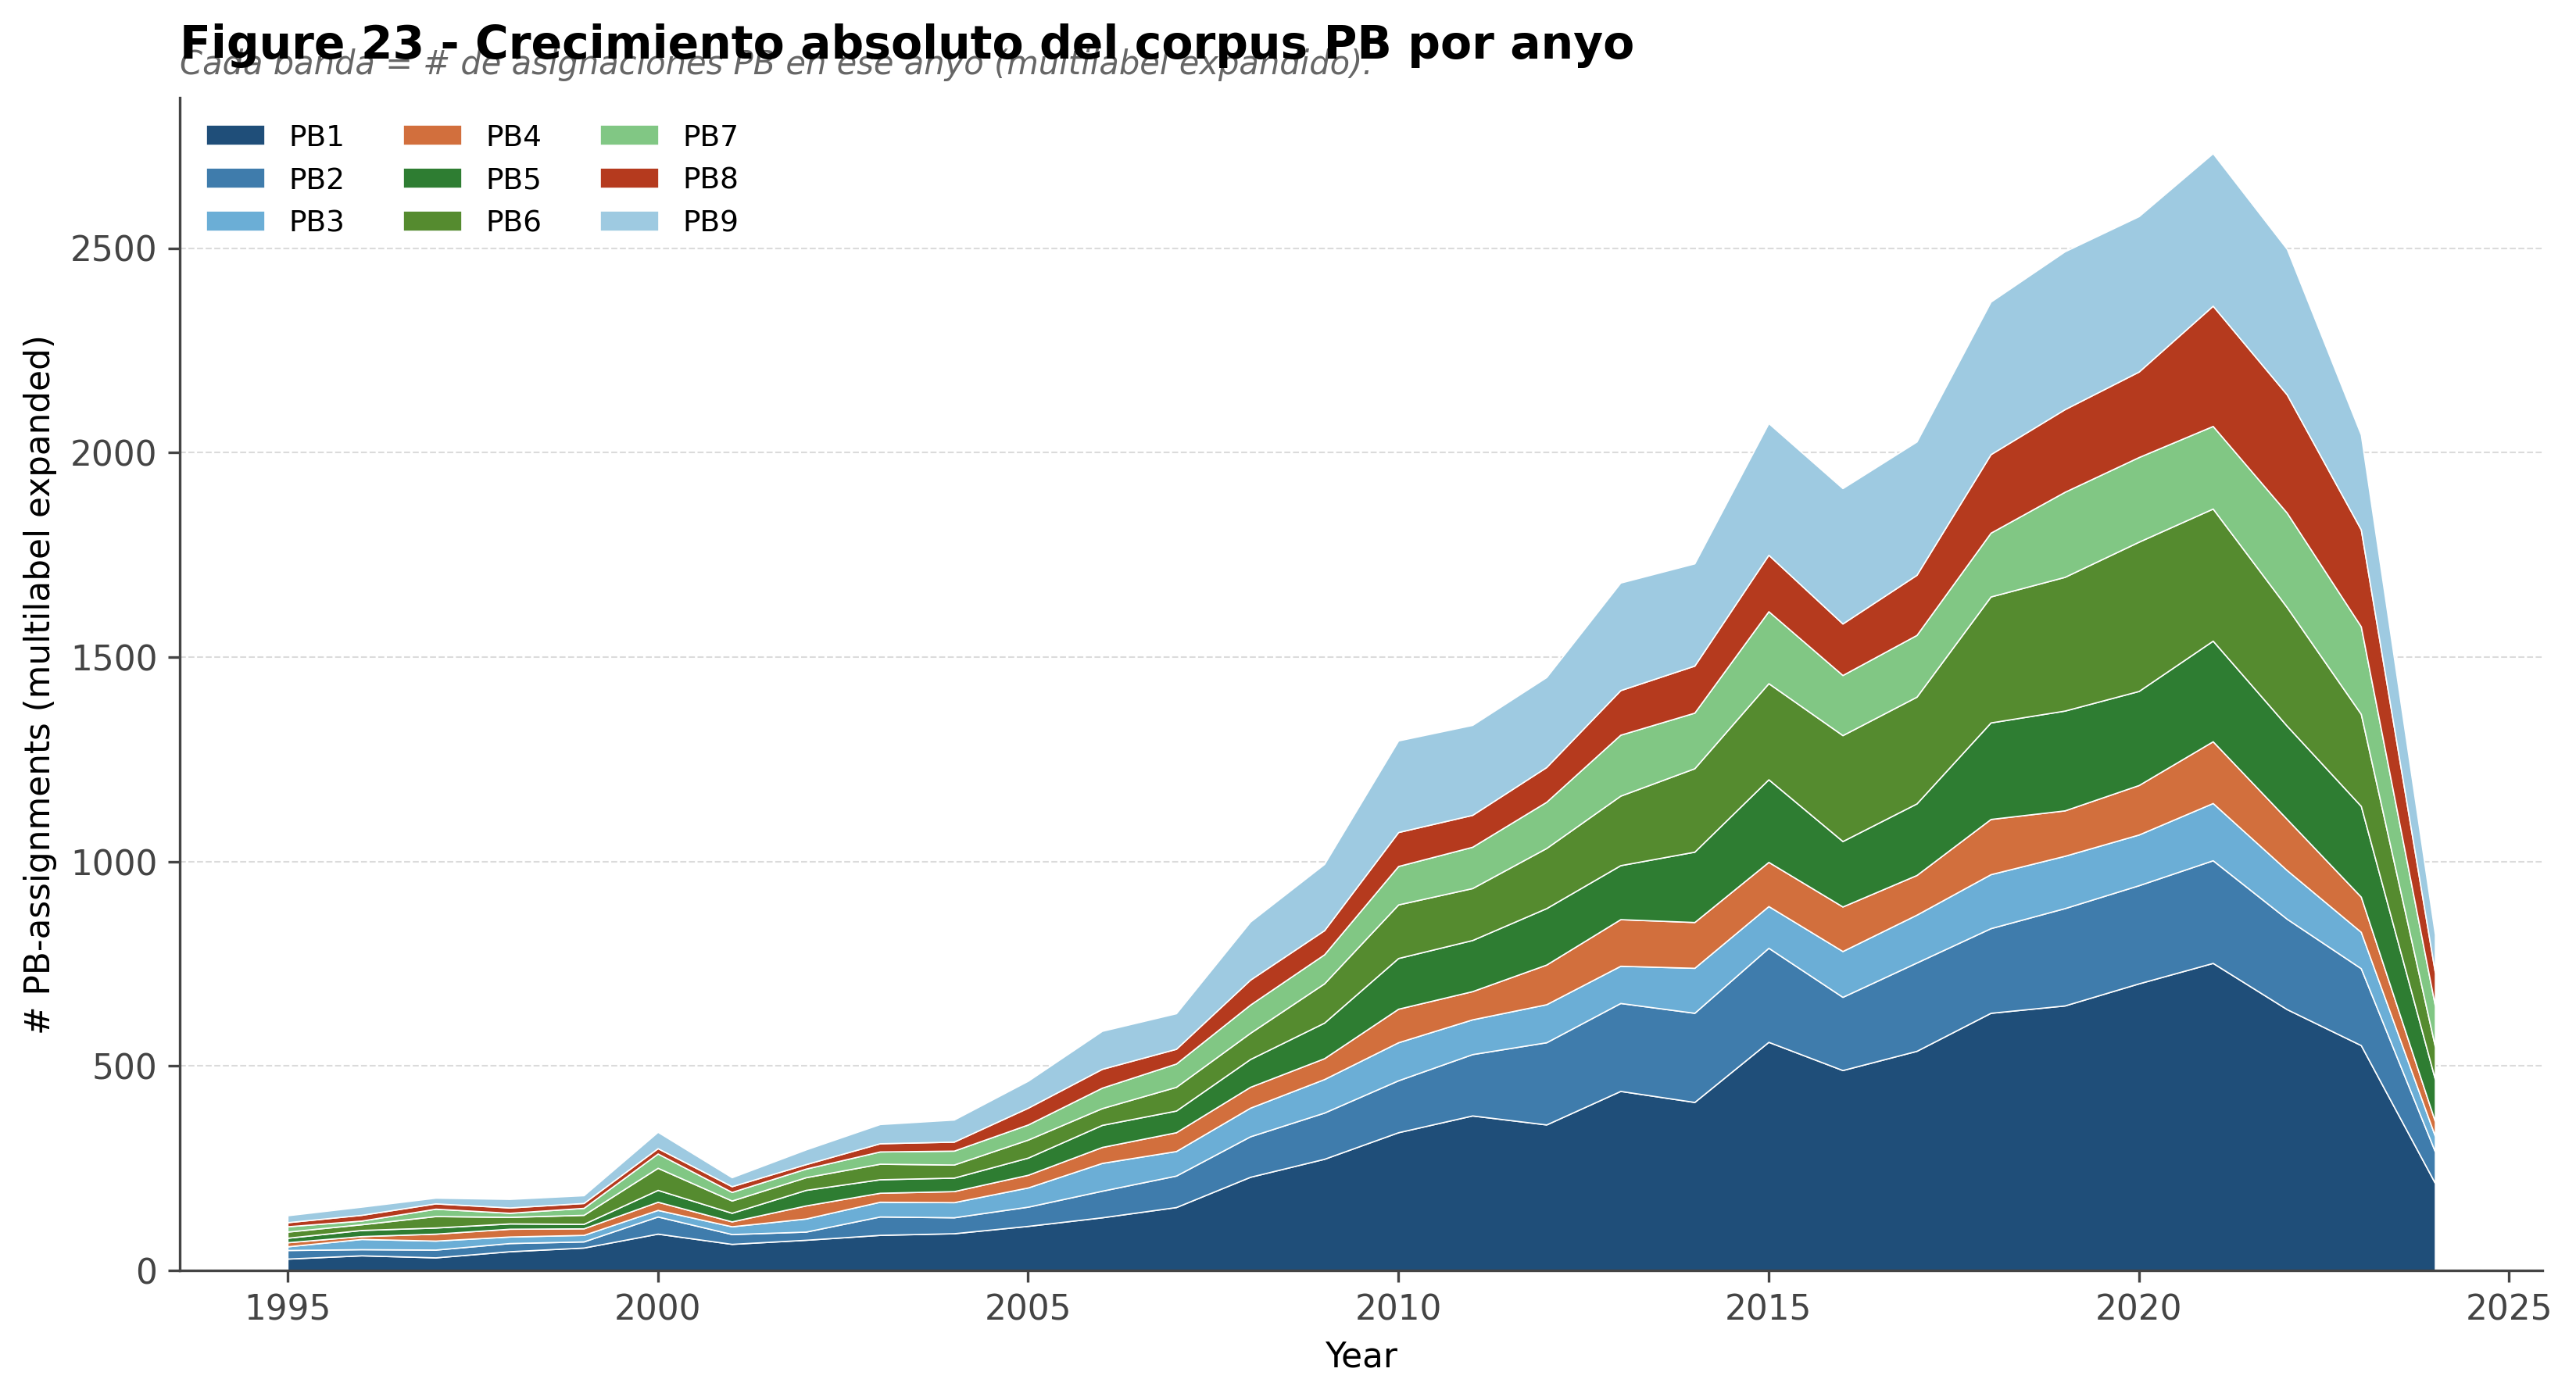
\includegraphics[width=\linewidth]{figures/23_stacked_area_absolute.png}
\caption{Volumen absoluto por PB y año.}
\end{subfigure}
\hfill
\begin{subfigure}{0.49\linewidth}
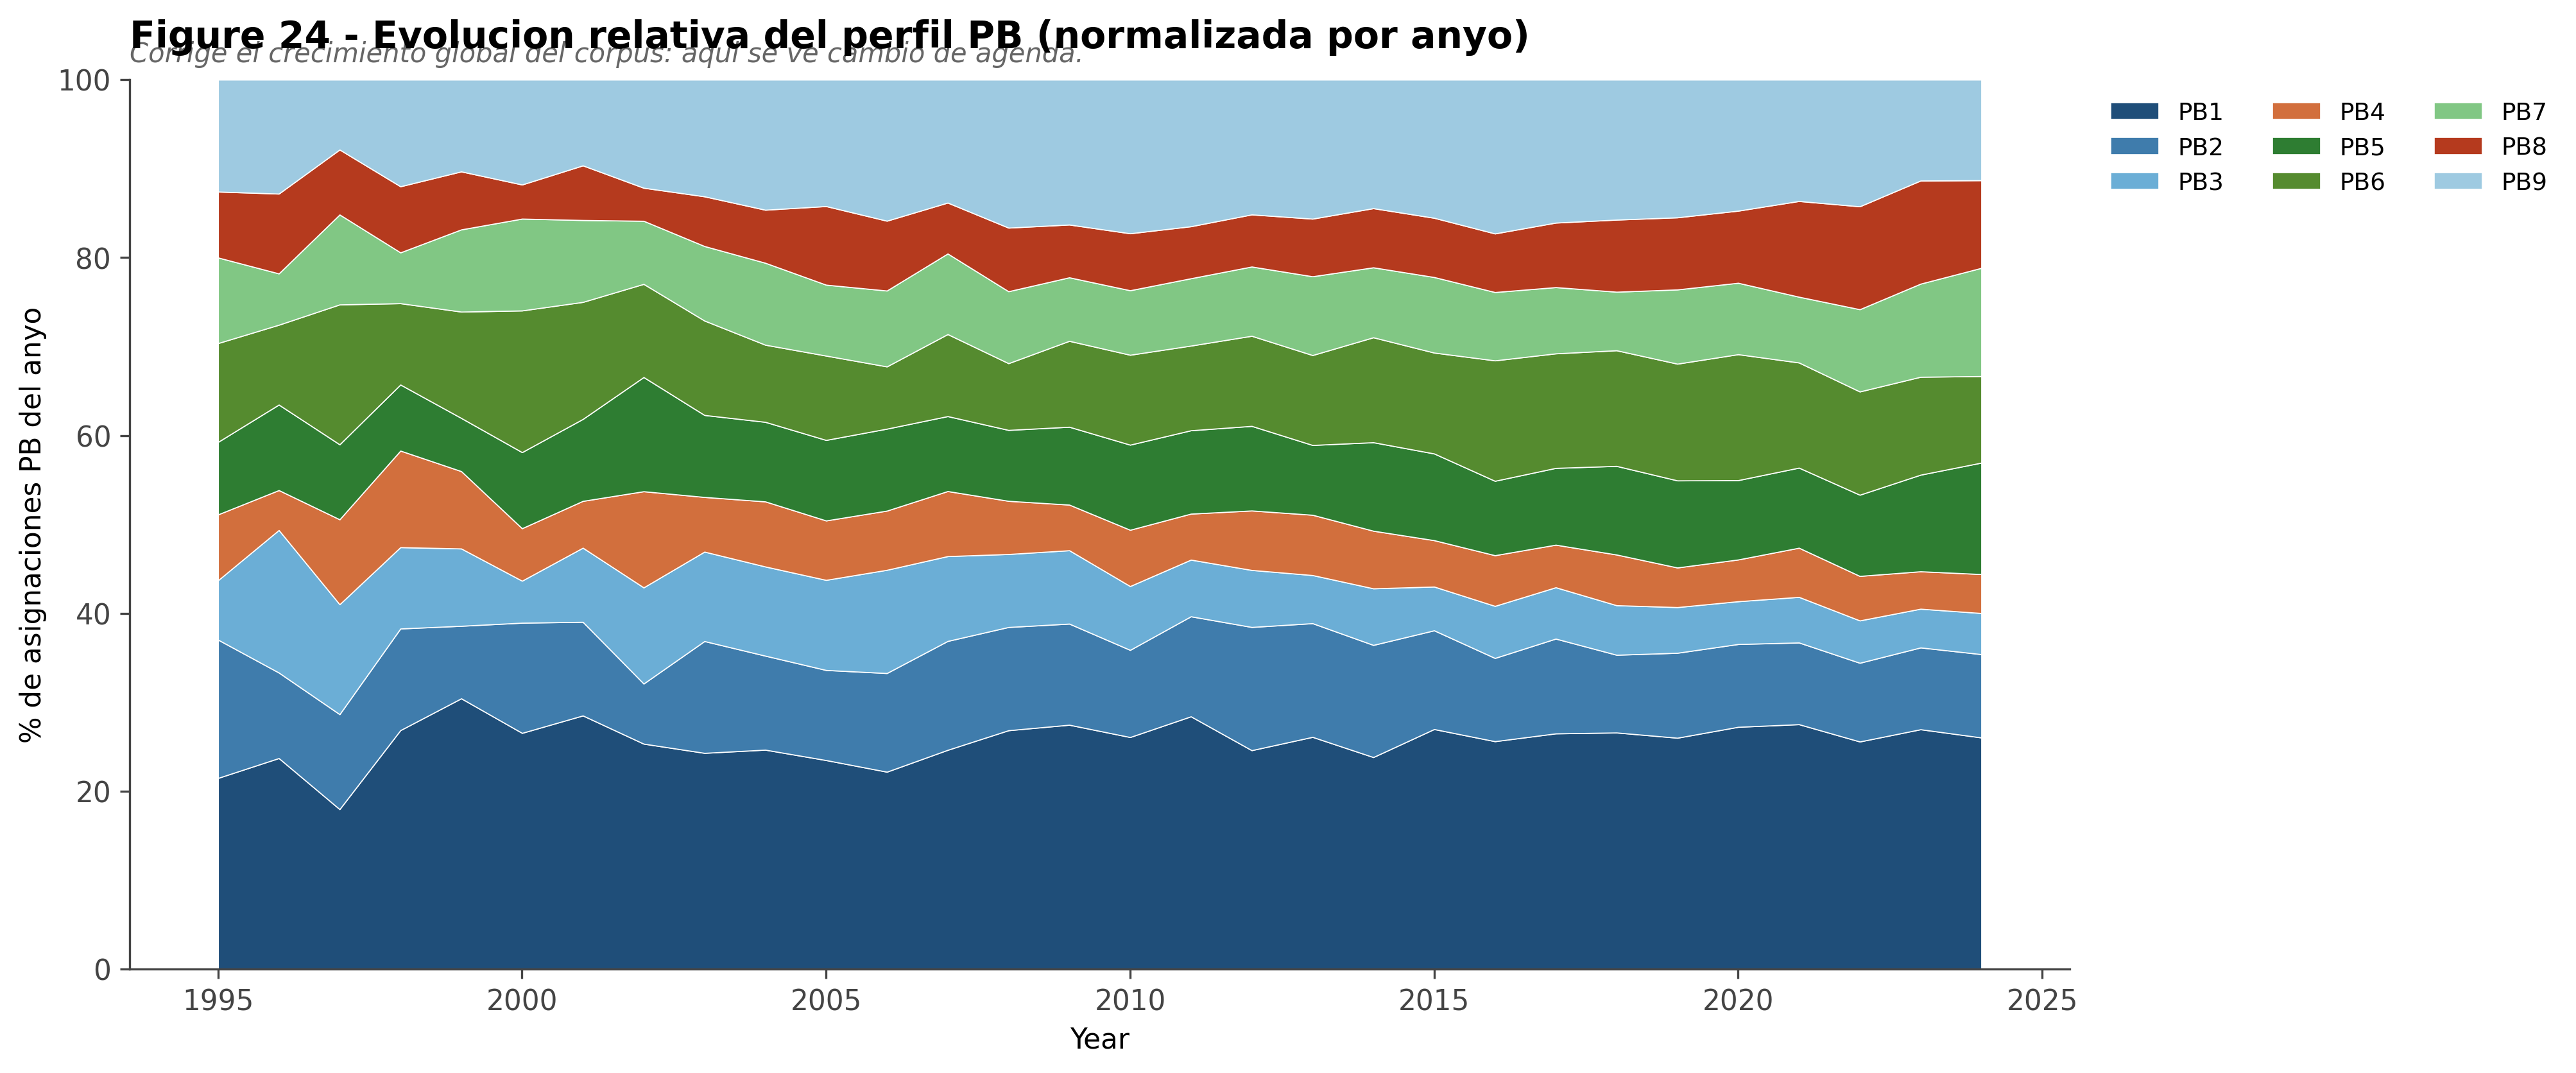
\includegraphics[width=\linewidth]{figures/24_streamgraph_normalized.png}
\caption{\% del año por PB (corrige crecimiento global).}
\end{subfigure}
\caption{Evolución temporal: absoluta vs normalizada.}
\label{fig:temporal_abs}
\end{figure}

\subsection{Comparativa por periodos}

\begin{figure}[h]
\centering
\begin{subfigure}{\linewidth}
\centering
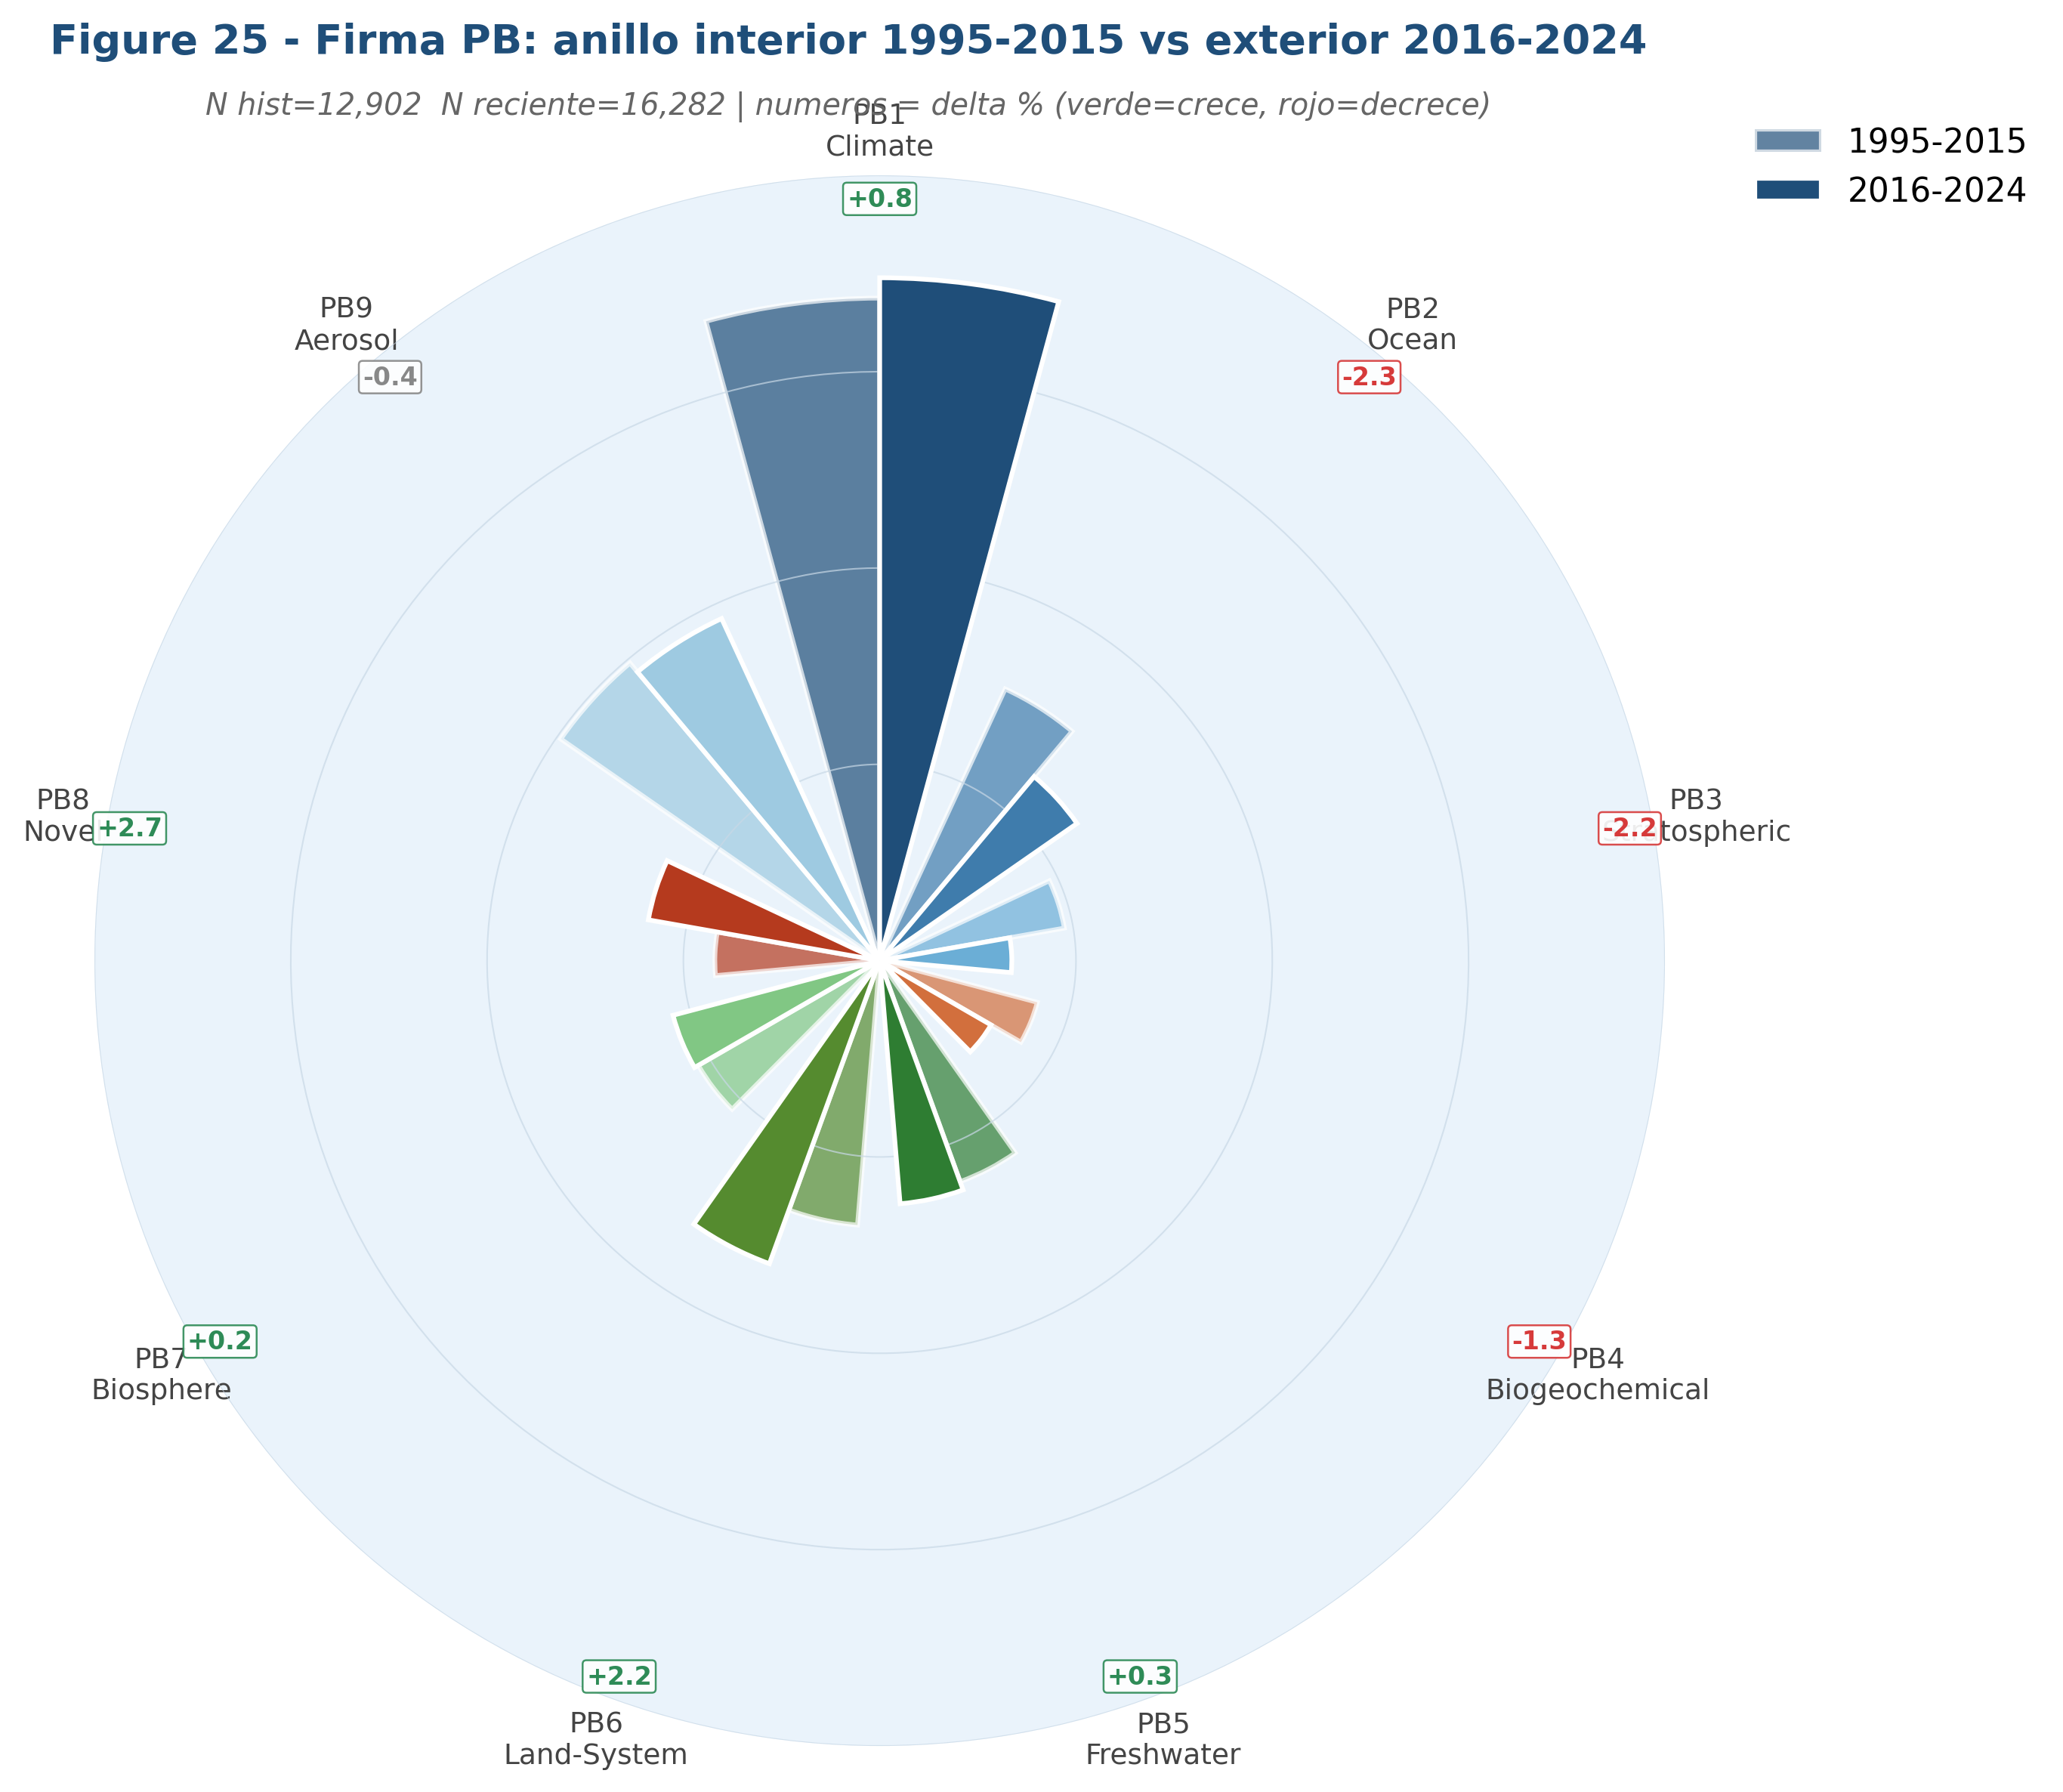
\includegraphics[width=0.7\linewidth]{figures/25_radial_doublelayer.png}
\caption{Radial doble capa: 1995--2015 (interior) vs 2016--2024 (exterior).}
\end{subfigure}\\[0.4em]
\begin{subfigure}{\linewidth}
\centering
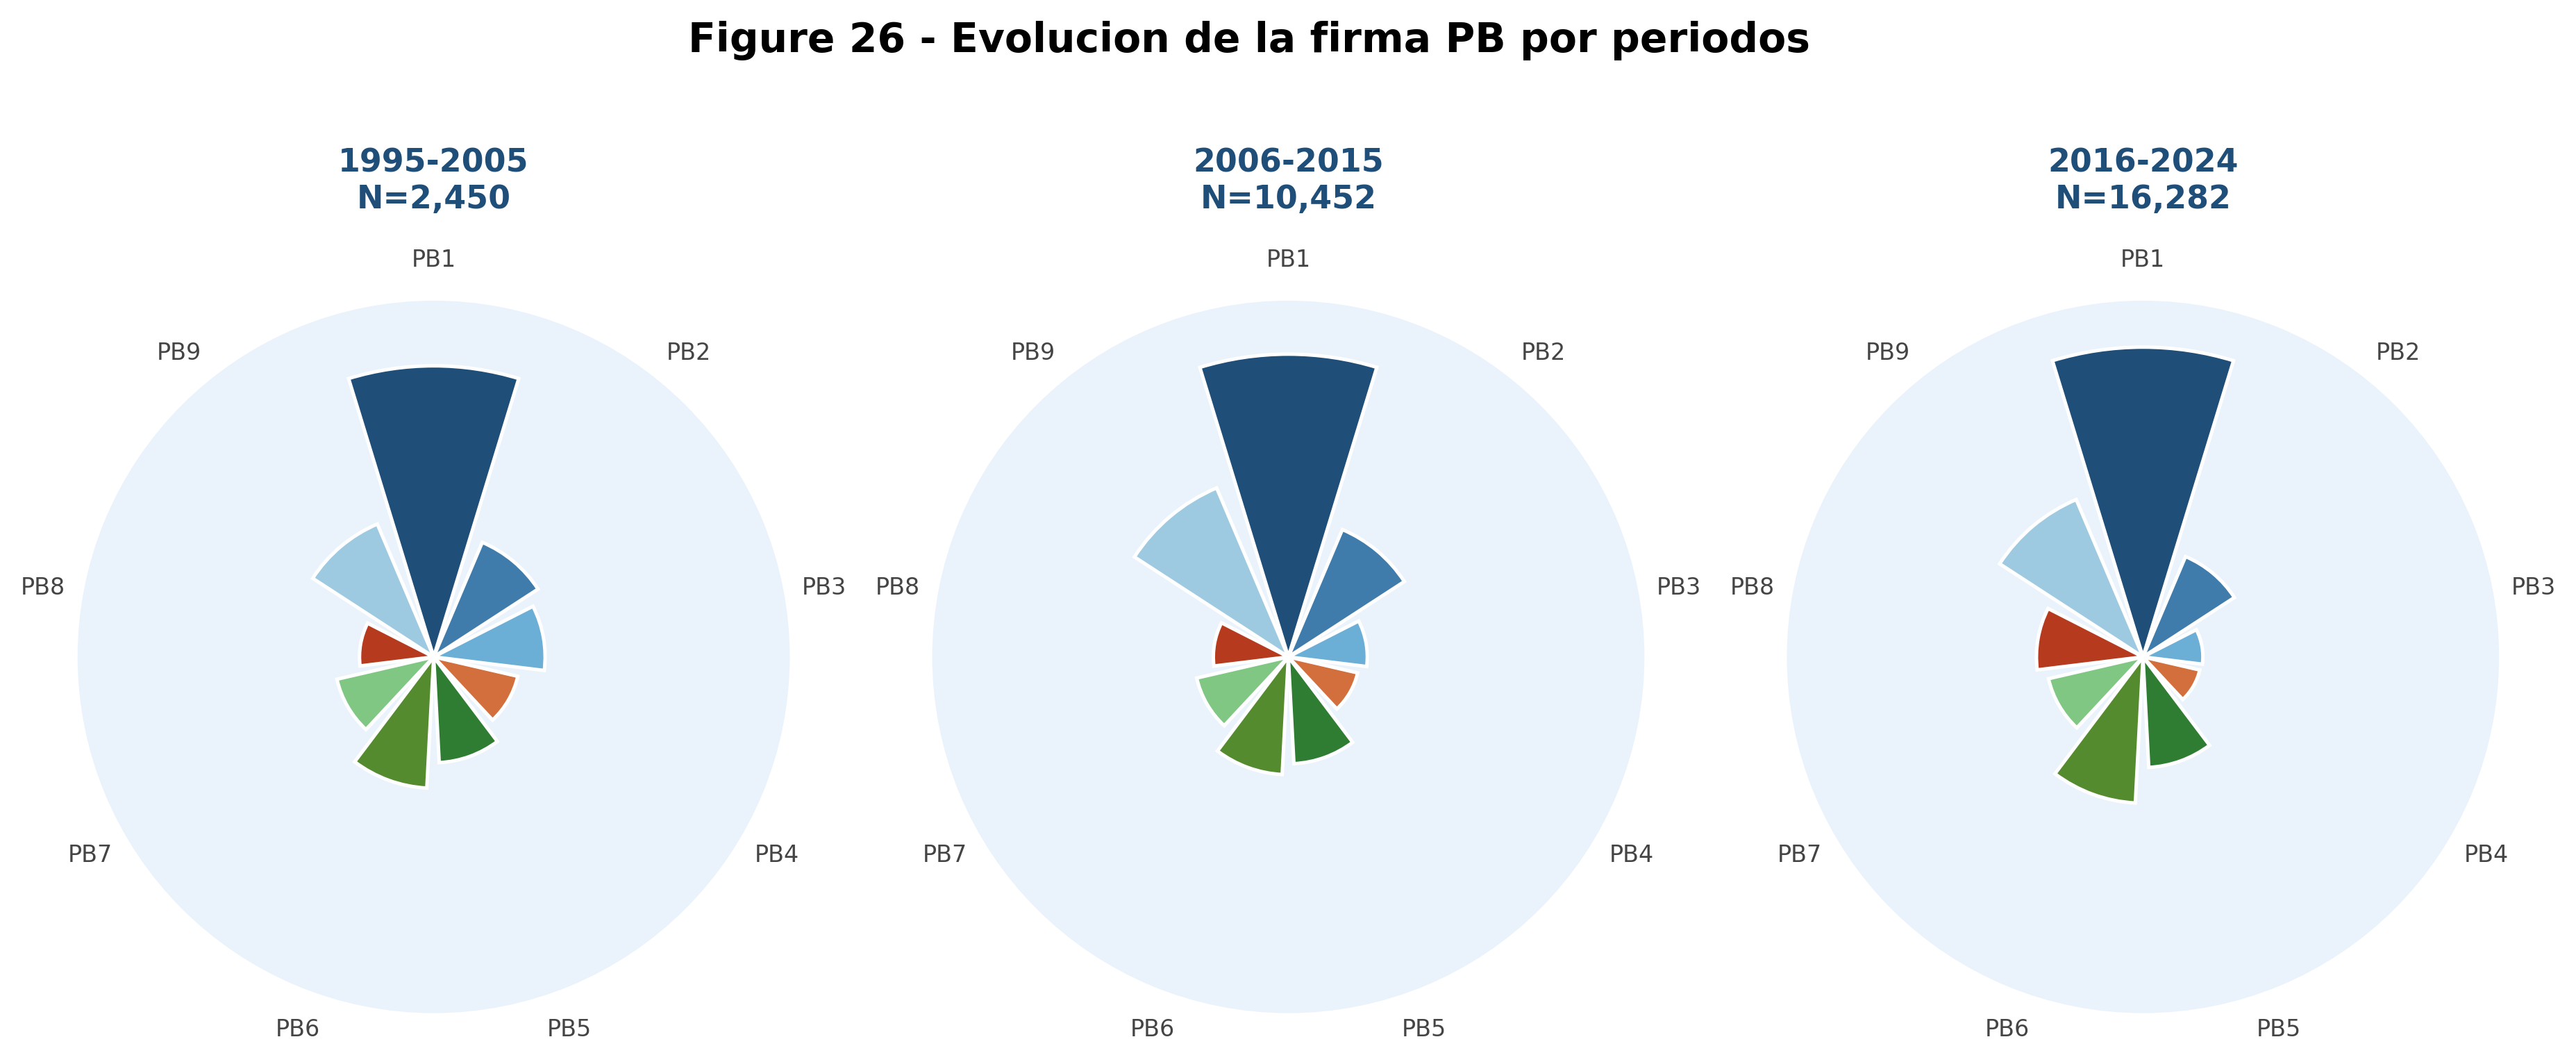
\includegraphics[width=0.92\linewidth]{figures/26_radial_small_multiples.png}
\caption{\emph{Small multiples} por periodo (1995--2005, 2006--2015, 2016--2024).}
\end{subfigure}
\caption{Tres ventanas temporales del perfil PB de la UPV. La transición clave es 2010--2015 $\to$ 2016--2020, coincidente con la Agenda 2030.}
\label{fig:temporal_radial}
\end{figure}

\paragraph{Observaciones temporales:}
\begin{itemize}
\item \pb1 se consolida como dominante desde 2005 y crece tras Paris/Agenda 2030.
\item \pb9 (aerosoles) dominó 2006--2015 (era MODIS/AERONET); su peso relativo desciende después.
\item \pb6 crece de forma sostenida pero sin picos: es tema de fondo, no de moda.
\item \pb8 apenas existía pre-2015 y emerge débilmente tras la Agenda 2030: hay reacción institucional pero con retraso de $\sim$2--3 años respecto a los \emph{frameworks} de política global, coherente con los tiempos de revisión y publicación.
\end{itemize}

% ============================================================
\section{Estructura sistémica: coocurrencias y red PB}\label{sec:sistemico}

\subsection{Multi-labelidad}

\begin{figure}[h]
\centering
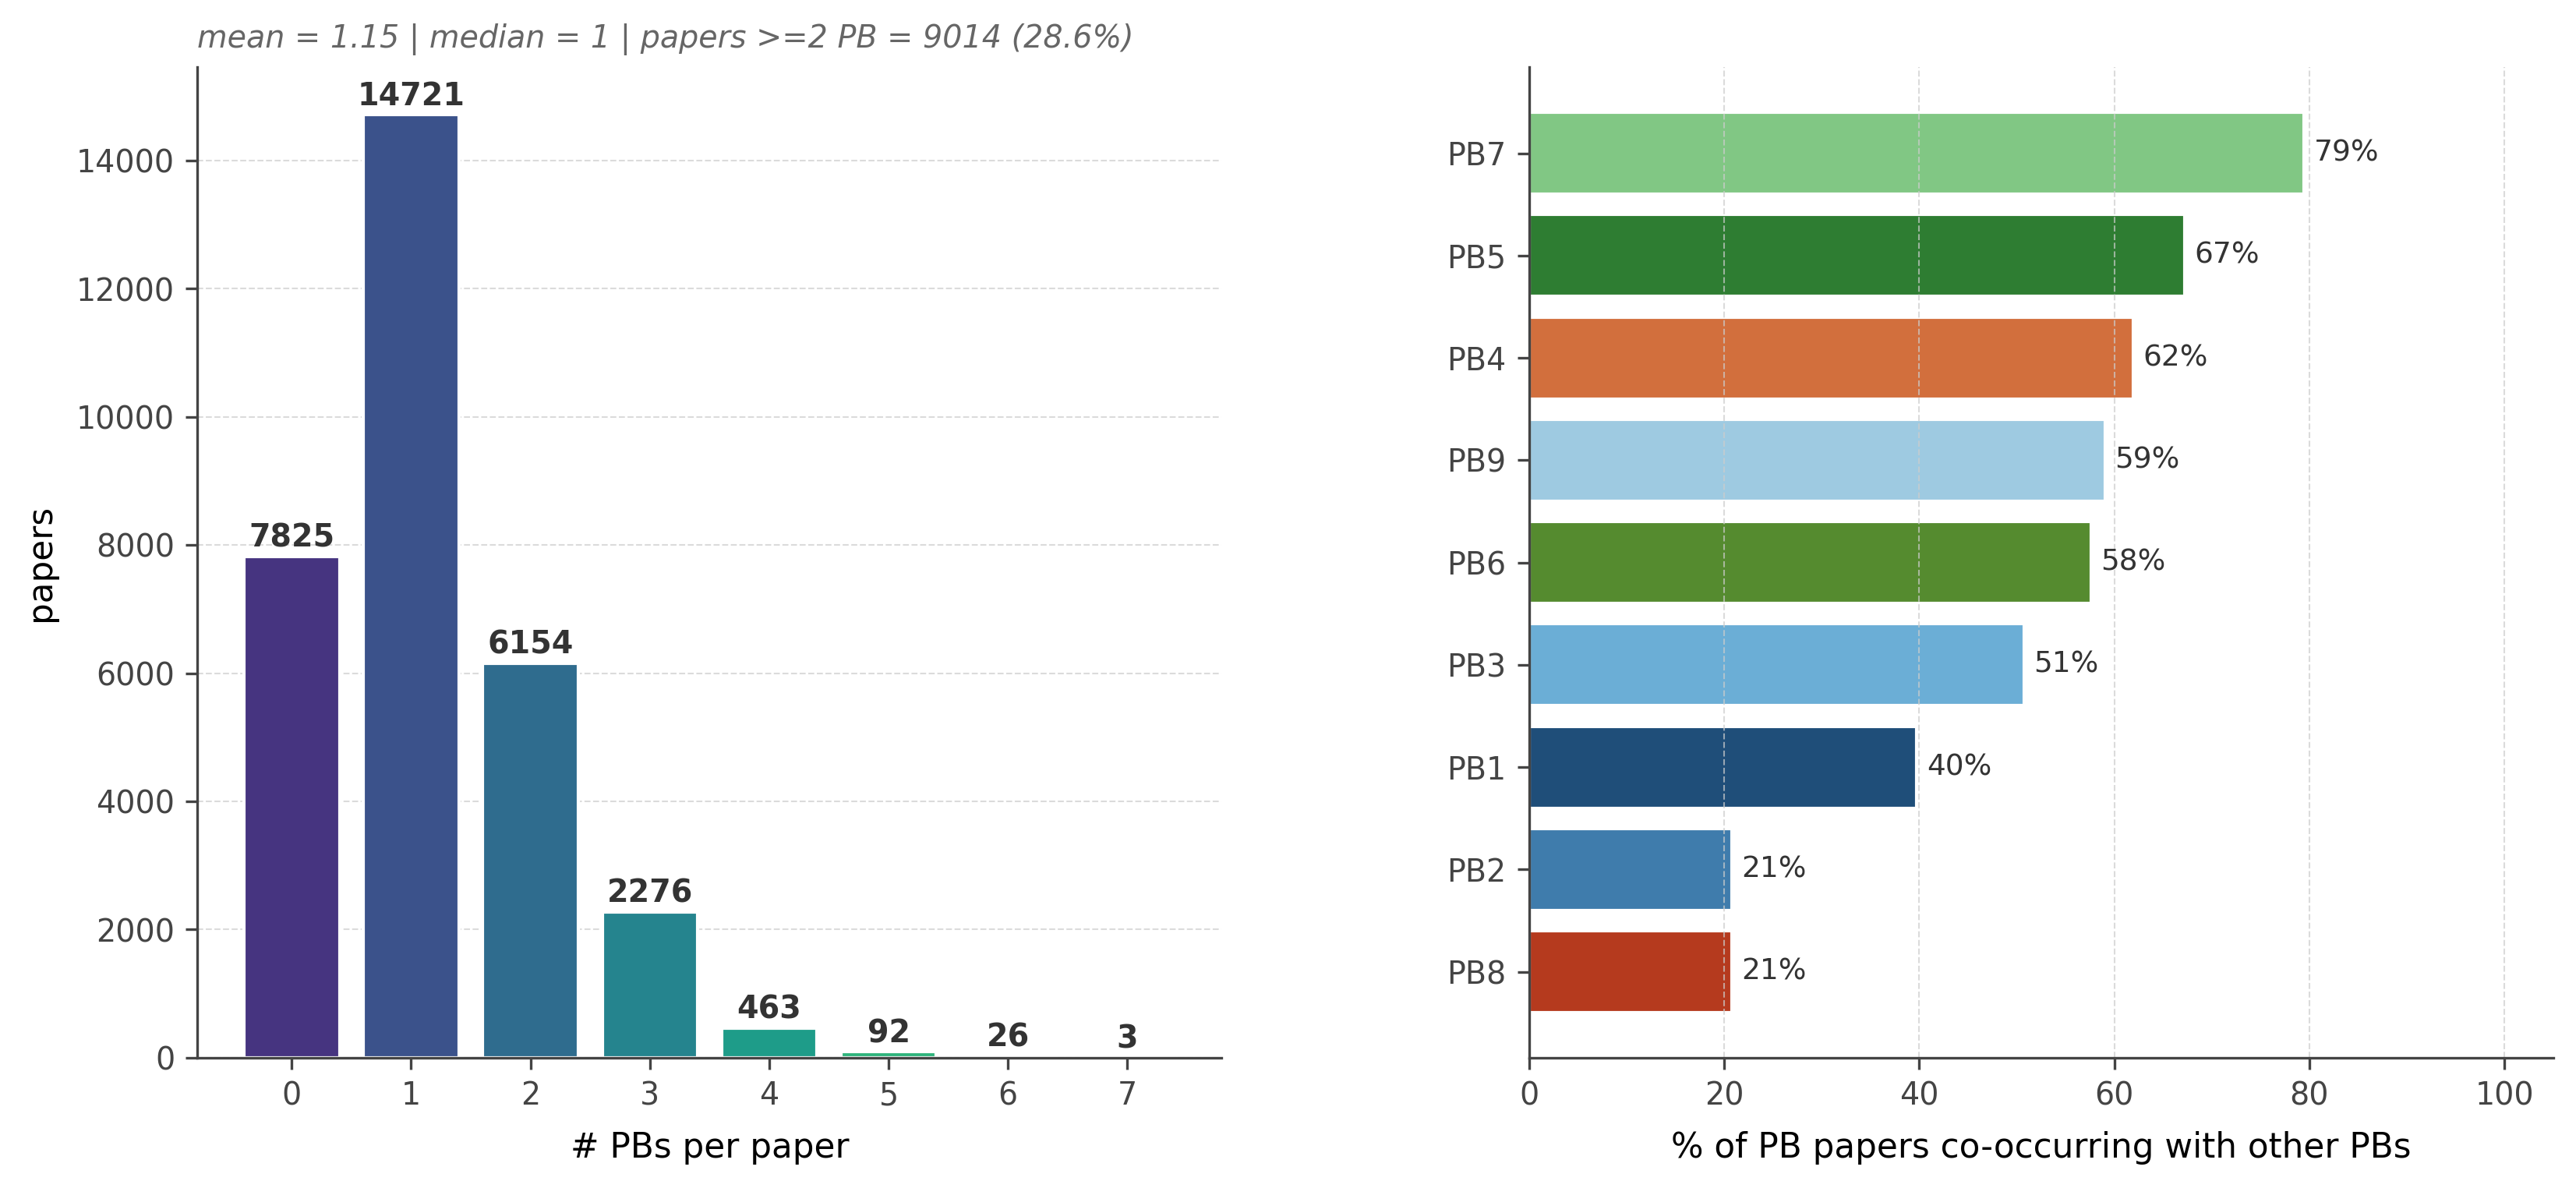
\includegraphics[width=0.95\linewidth]{figures/06_pb_multilabel.png}
\caption{Estructura multilabel: \textbf{(a)} histograma de PBs por paper (mediana $=1$, $\sim 28\,\%$ con $\geq 2$ PBs); \textbf{(b)} \% de papers de cada PB que aparecen acompañados.}
\label{fig:multi}
\end{figure}

El $28\,\%$ de los papers toca al menos dos PBs simultáneamente, lo que justifica el tratamiento multilabel. PBs como \pb4 y \pb5 son los más \emph{sistémicos} (rara vez aparecen aislados), mientras que \pb1 y \pb2 son los más \emph{monotemáticos}, coherente con sus subculturas disciplinares maduras (climatología, oceanografía).

\subsection{Coocurrencias y asociación normalizada (Jaccard)}

Las coocurrencias brutas favorecen mecánicamente a los PBs grandes. Para una asociación normalizada usamos el coeficiente de Jaccard:
\begin{equation}
J(\text{PB}_i, \text{PB}_j) = \frac{|D_i \cap D_j|}{|D_i \cup D_j|}
\end{equation}
donde $D_k$ es el conjunto de documentos asignados al PB $k$. La Figura~\ref{fig:co} muestra ambas matrices.

\begin{figure}[h]
\centering
\begin{subfigure}{\linewidth}
\centering
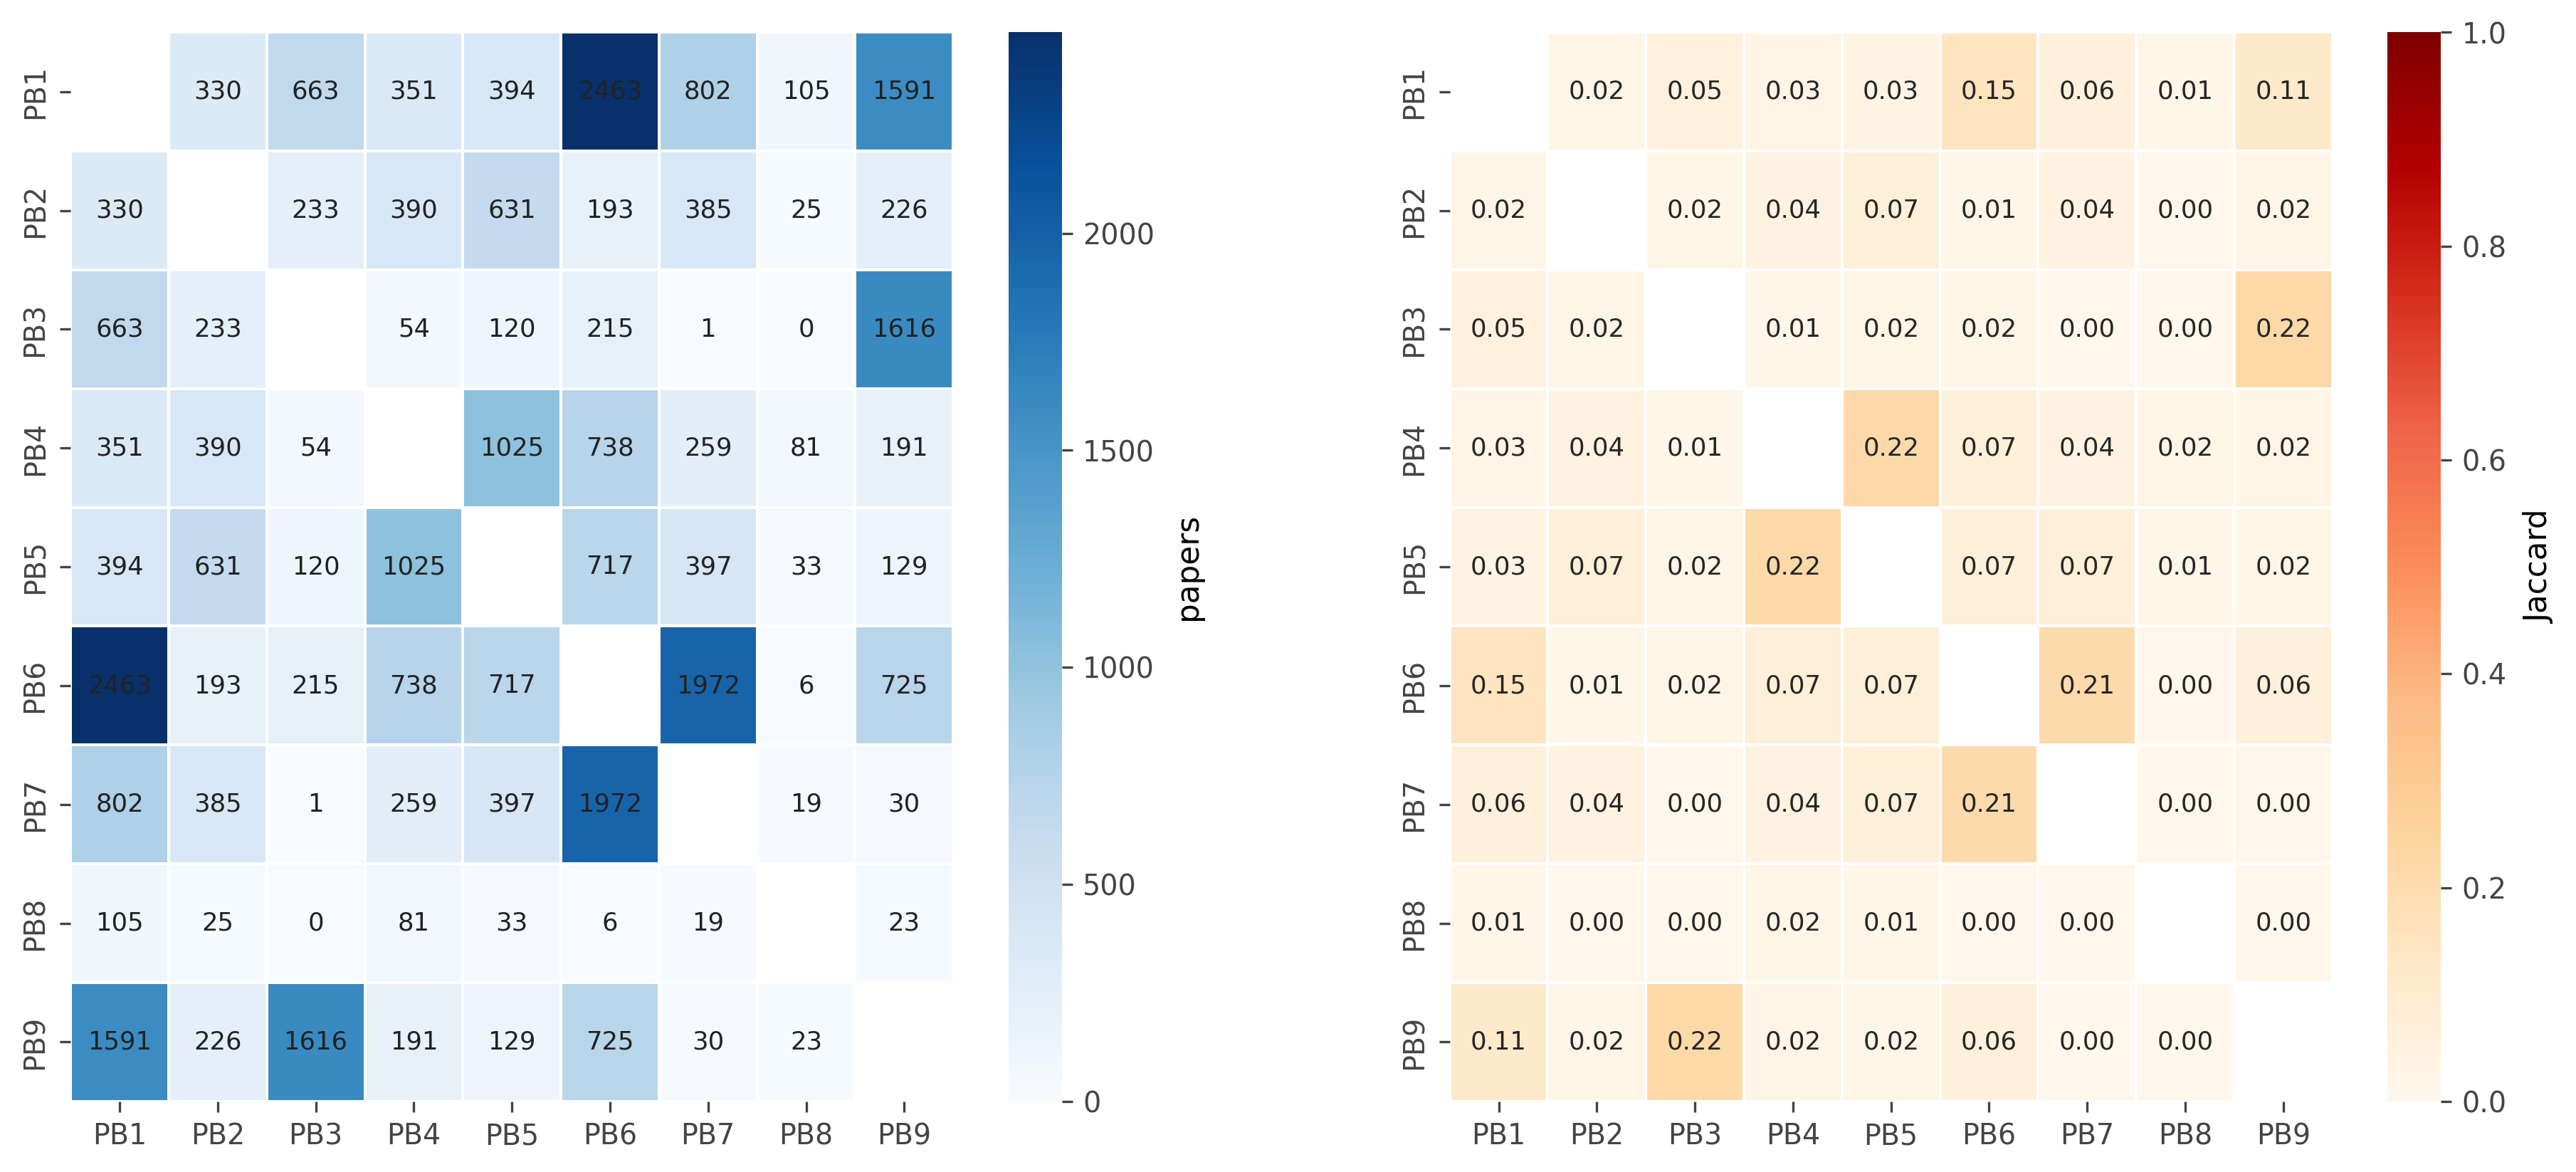
\includegraphics[width=0.95\linewidth]{figures/03_pb_cooccurrence_heatmaps.png}
\caption{Heatmap de coocurrencia (izq.\ bruto, dcha.\ Jaccard normalizado).}
\end{subfigure}\\[0.5em]
\begin{subfigure}{\linewidth}
\centering
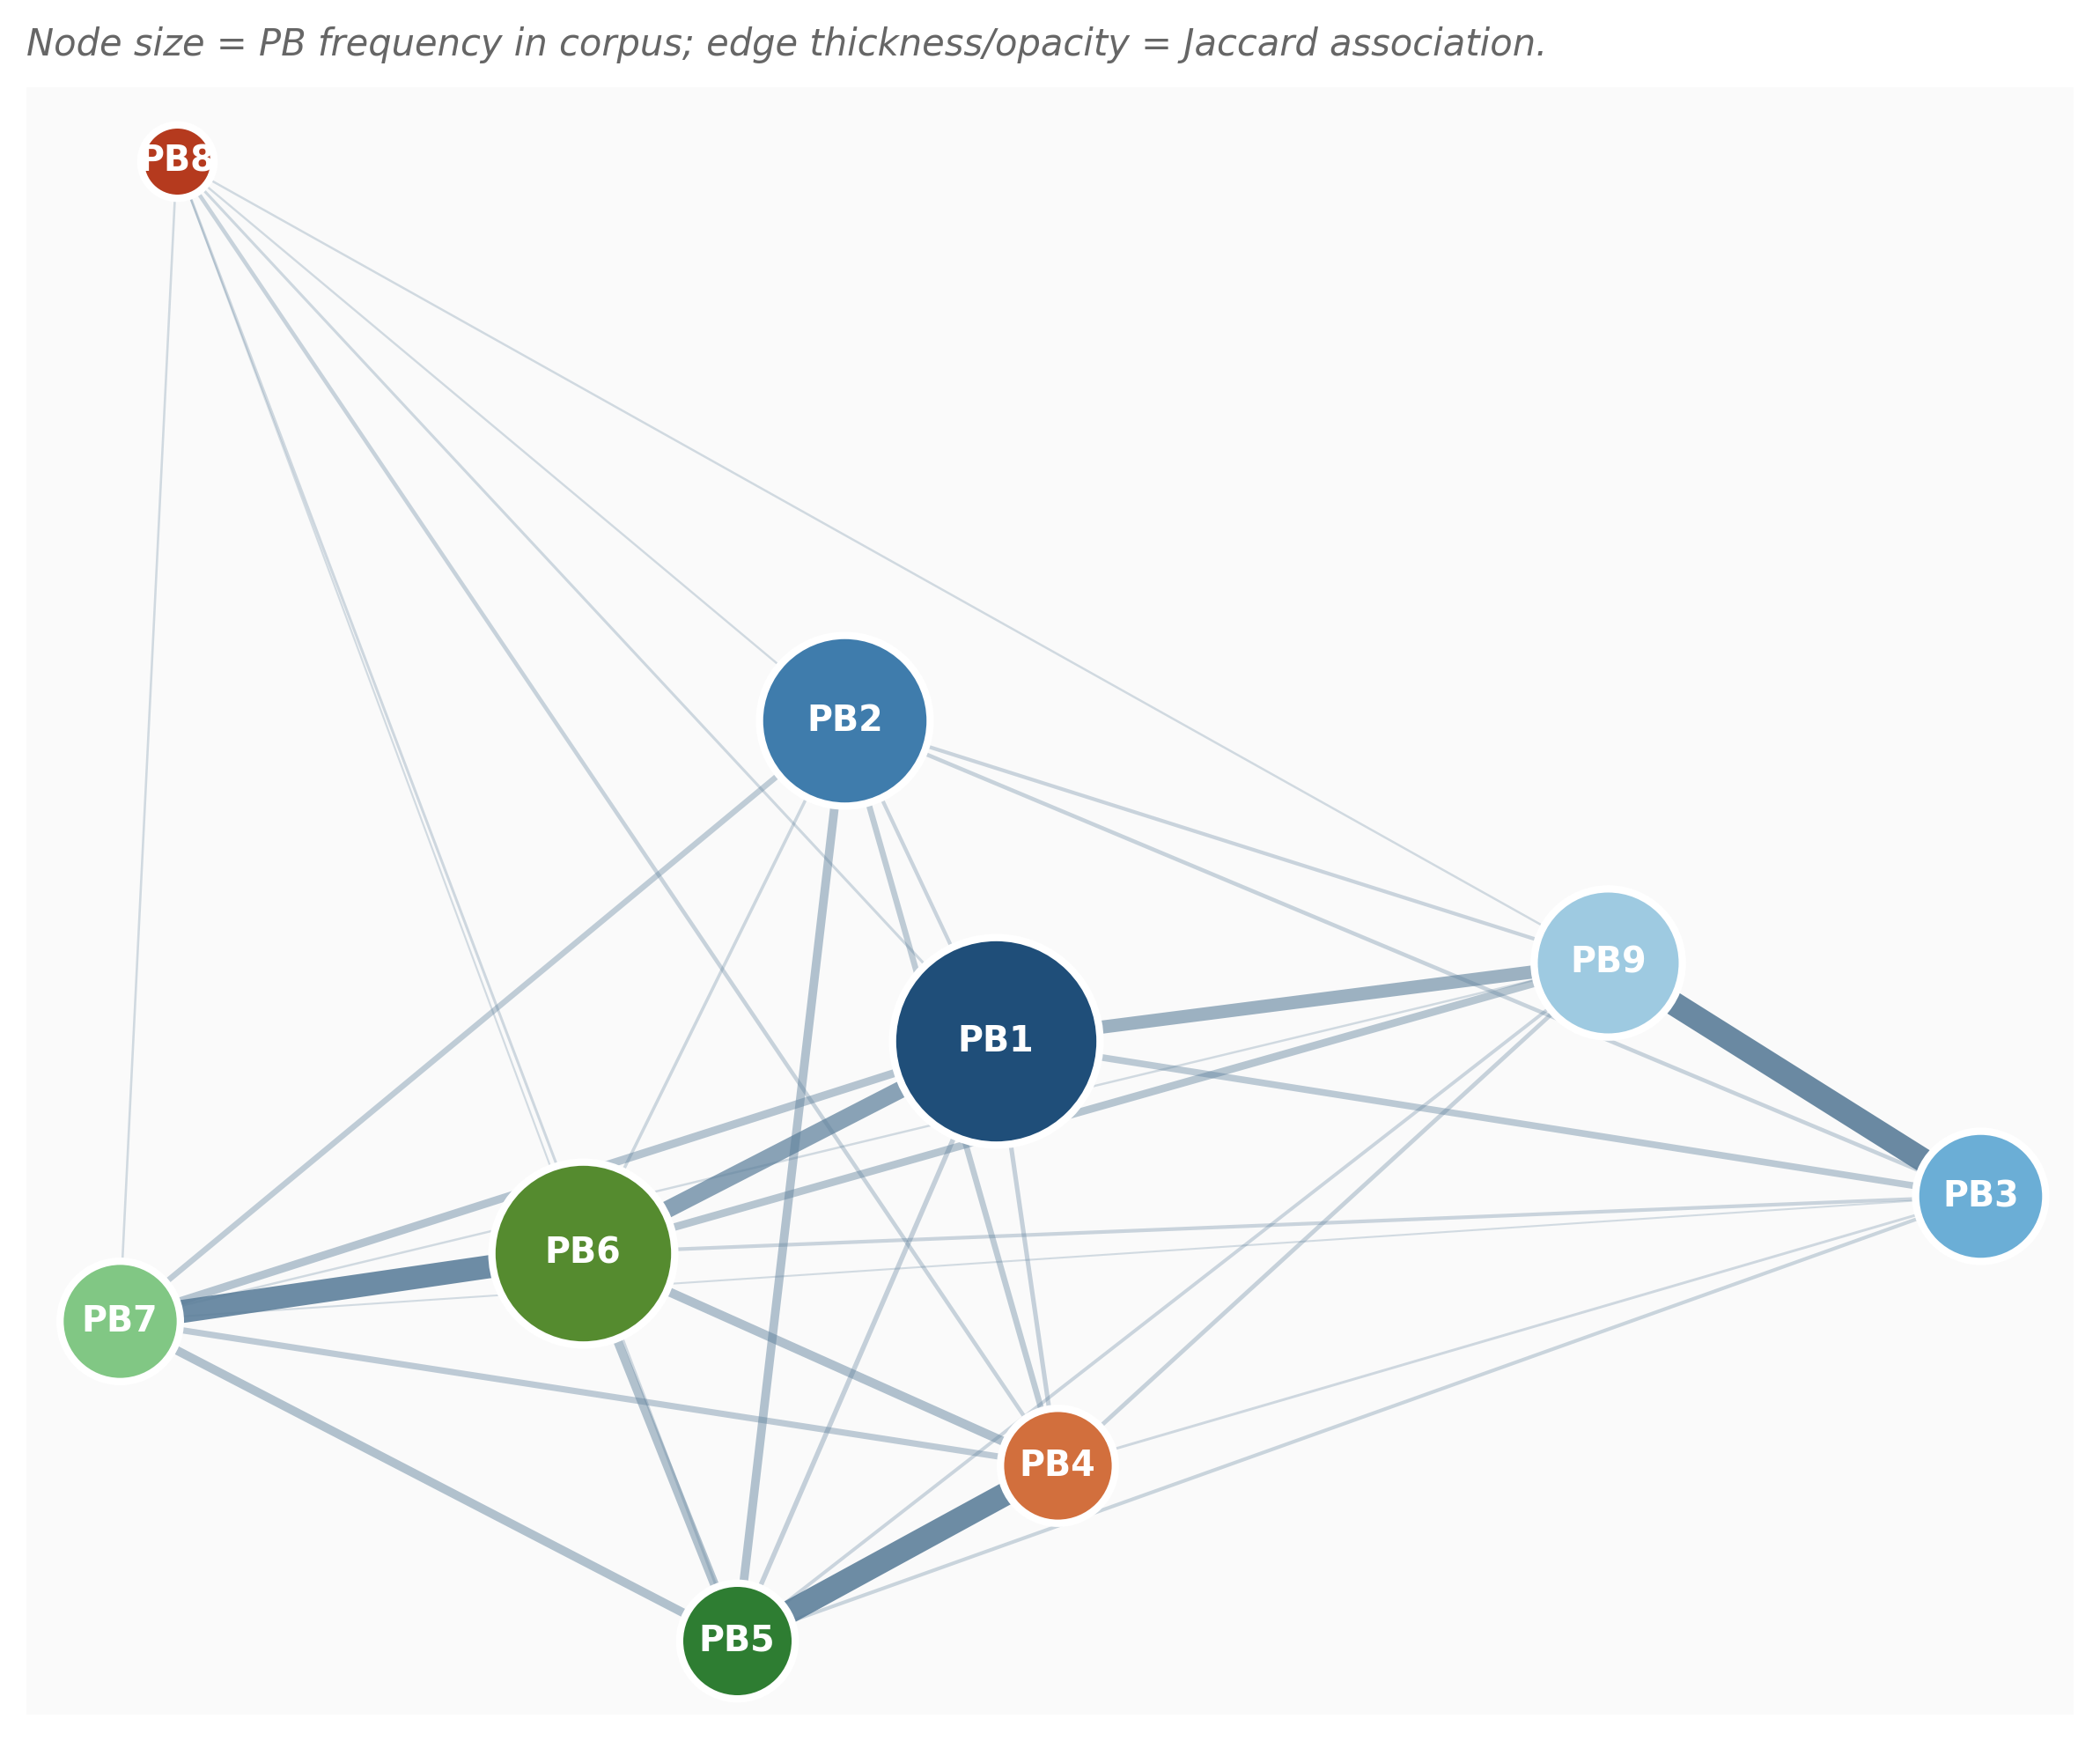
\includegraphics[width=0.7\linewidth]{figures/04_pb_network.png}
\caption{Red PB: nodos $=$ PBs, tamaño $\propto$ frecuencia, aristas $\propto$ Jaccard.}
\end{subfigure}
\caption{Estructura sistémica de los PBs en el corpus UPV.}
\label{fig:co}
\end{figure}

\begin{table}[h]
\centering\small
\begin{tabular}{l c r r}
\toprule
\textbf{Pareja} & \textbf{Jaccard} & \textbf{Coocurr.} & \textbf{Interpretación física} \\
\midrule
\good{\pb3 $\leftrightarrow$ \pb9} & 0{,}221 & \num{1616} & Ozono y aerosoles: misma física atmosférica \\
\good{\pb4 $\leftrightarrow$ \pb5} & 0{,}215 & \num{1025} & Ciclos N/P llegan a masas de agua dulce \\
\good{\pb6 $\leftrightarrow$ \pb7} & 0{,}213 & \num{1972} & Land-use change arrastra biosfera \\
\pb1 $\leftrightarrow$ \pb6 & 0{,}154 & \num{2463} & Deforestación como driver climático \\
\pb1 $\leftrightarrow$ \pb9 & 0{,}114 & \num{1591} & Aerosoles en forzamiento radiativo \\
\bottomrule
\end{tabular}
\caption{Top-5 parejas con mayor Jaccard. Las tres primeras son \textbf{interacciones físicamente esperadas} entre PBs; el AED las recupera sin imponerlas.}
\label{tab:jaccard}
\end{table}

\subsection{Centralidad y comunidades}

Sobre la red PB (Figura~\ref{fig:co}b) calculamos \emph{weighted degree} y \emph{betweenness centrality}. El resultado:

\begin{table}[h]
\centering\small
\begin{tabular}{l r r}
\toprule
\textbf{PB} & \textbf{Weighted degree} & \textbf{Betweenness} \\
\midrule
\pb6 & 0{,}540 & 0{,}000 \\
\pb9 & 0{,}518 & 0{,}071 \\
\pb1 & 0{,}458 & 0{,}143 \\
\pb5 & 0{,}424 & 0{,}000 \\
\pb7 & 0{,}415 & 0{,}000 \\
\bottomrule
\end{tabular}
\caption{Centralidad en la red PB. \pb1 y \pb9 son los únicos puentes (betweenness $>0$).}
\end{table}

\pb1 y \pb9 actúan como \textbf{puentes} entre las familias atmosférica y tierra/biosfera. \pb8 queda periférico, confirmando su desconexión del resto.

% ============================================================
\section{Estructura semántica del corpus}\label{sec:semantico}

\subsection{Mapa semántico UMAP}

Proyectamos los 31\,560 abstracts en 2D mediante UMAP \cite{mcinnes2018umap} sobre el vector de scores PB de SPECTER (9-dim $\to$ 2D, métrica cosine, normalizada). La proyección permite ver clusters temáticos y zonas mixtas.

\begin{figure}[h]
\centering
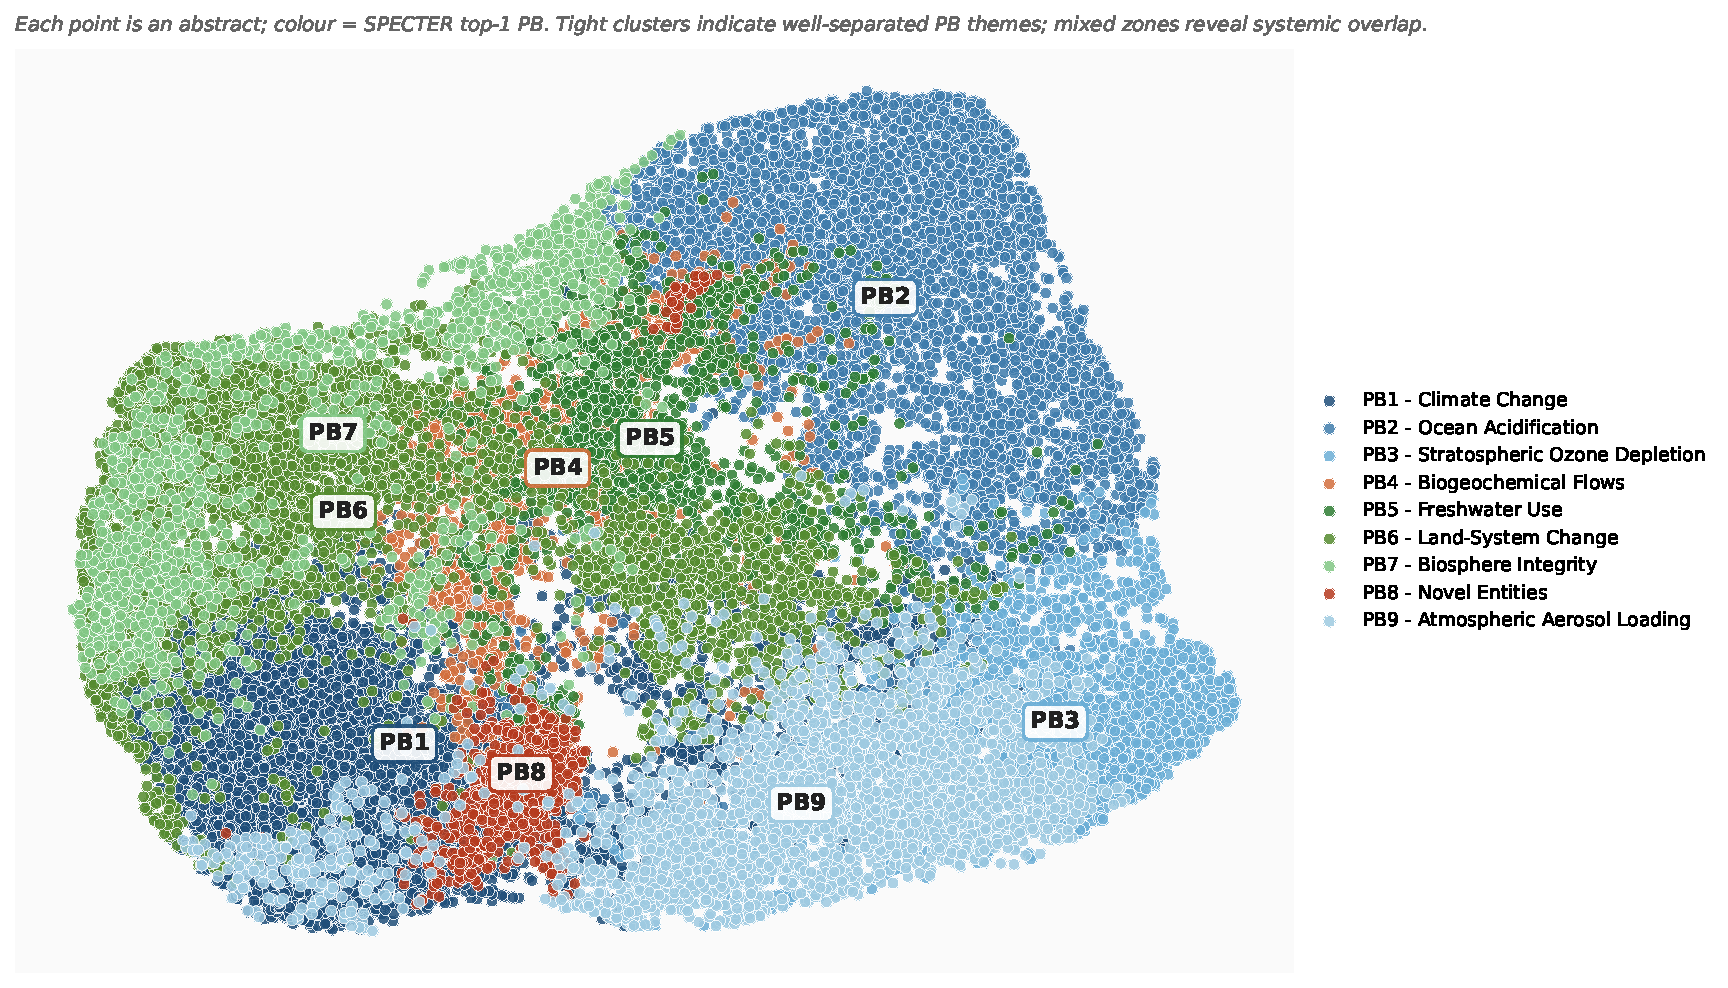
\includegraphics[width=0.85\linewidth]{figures/07_semantic_umap.png}
\caption{UMAP del corpus coloreado por PB top-1 (SPECTER). \pb1, \pb2 y \pb9 forman clusters separados; \pb6 y \pb7 forman continuo solapado (Jaccard alto coherente); \pb8 disperso (sin región semántica clara).}
\label{fig:umap}
\end{figure}

\subsection{Topics latentes y Sankey topics-PB}

Mediante \texttt{KMeans} ($K{=}8$) sobre los vectores de score TF-IDF normalizados extraemos clusters semánticos no supervisados y los etiquetamos por sus dos PBs dominantes (centroides). La Figura~\ref{fig:sankey} muestra el flujo cluster$\to$\pb{} top-1:

\begin{figure}[h]
\centering
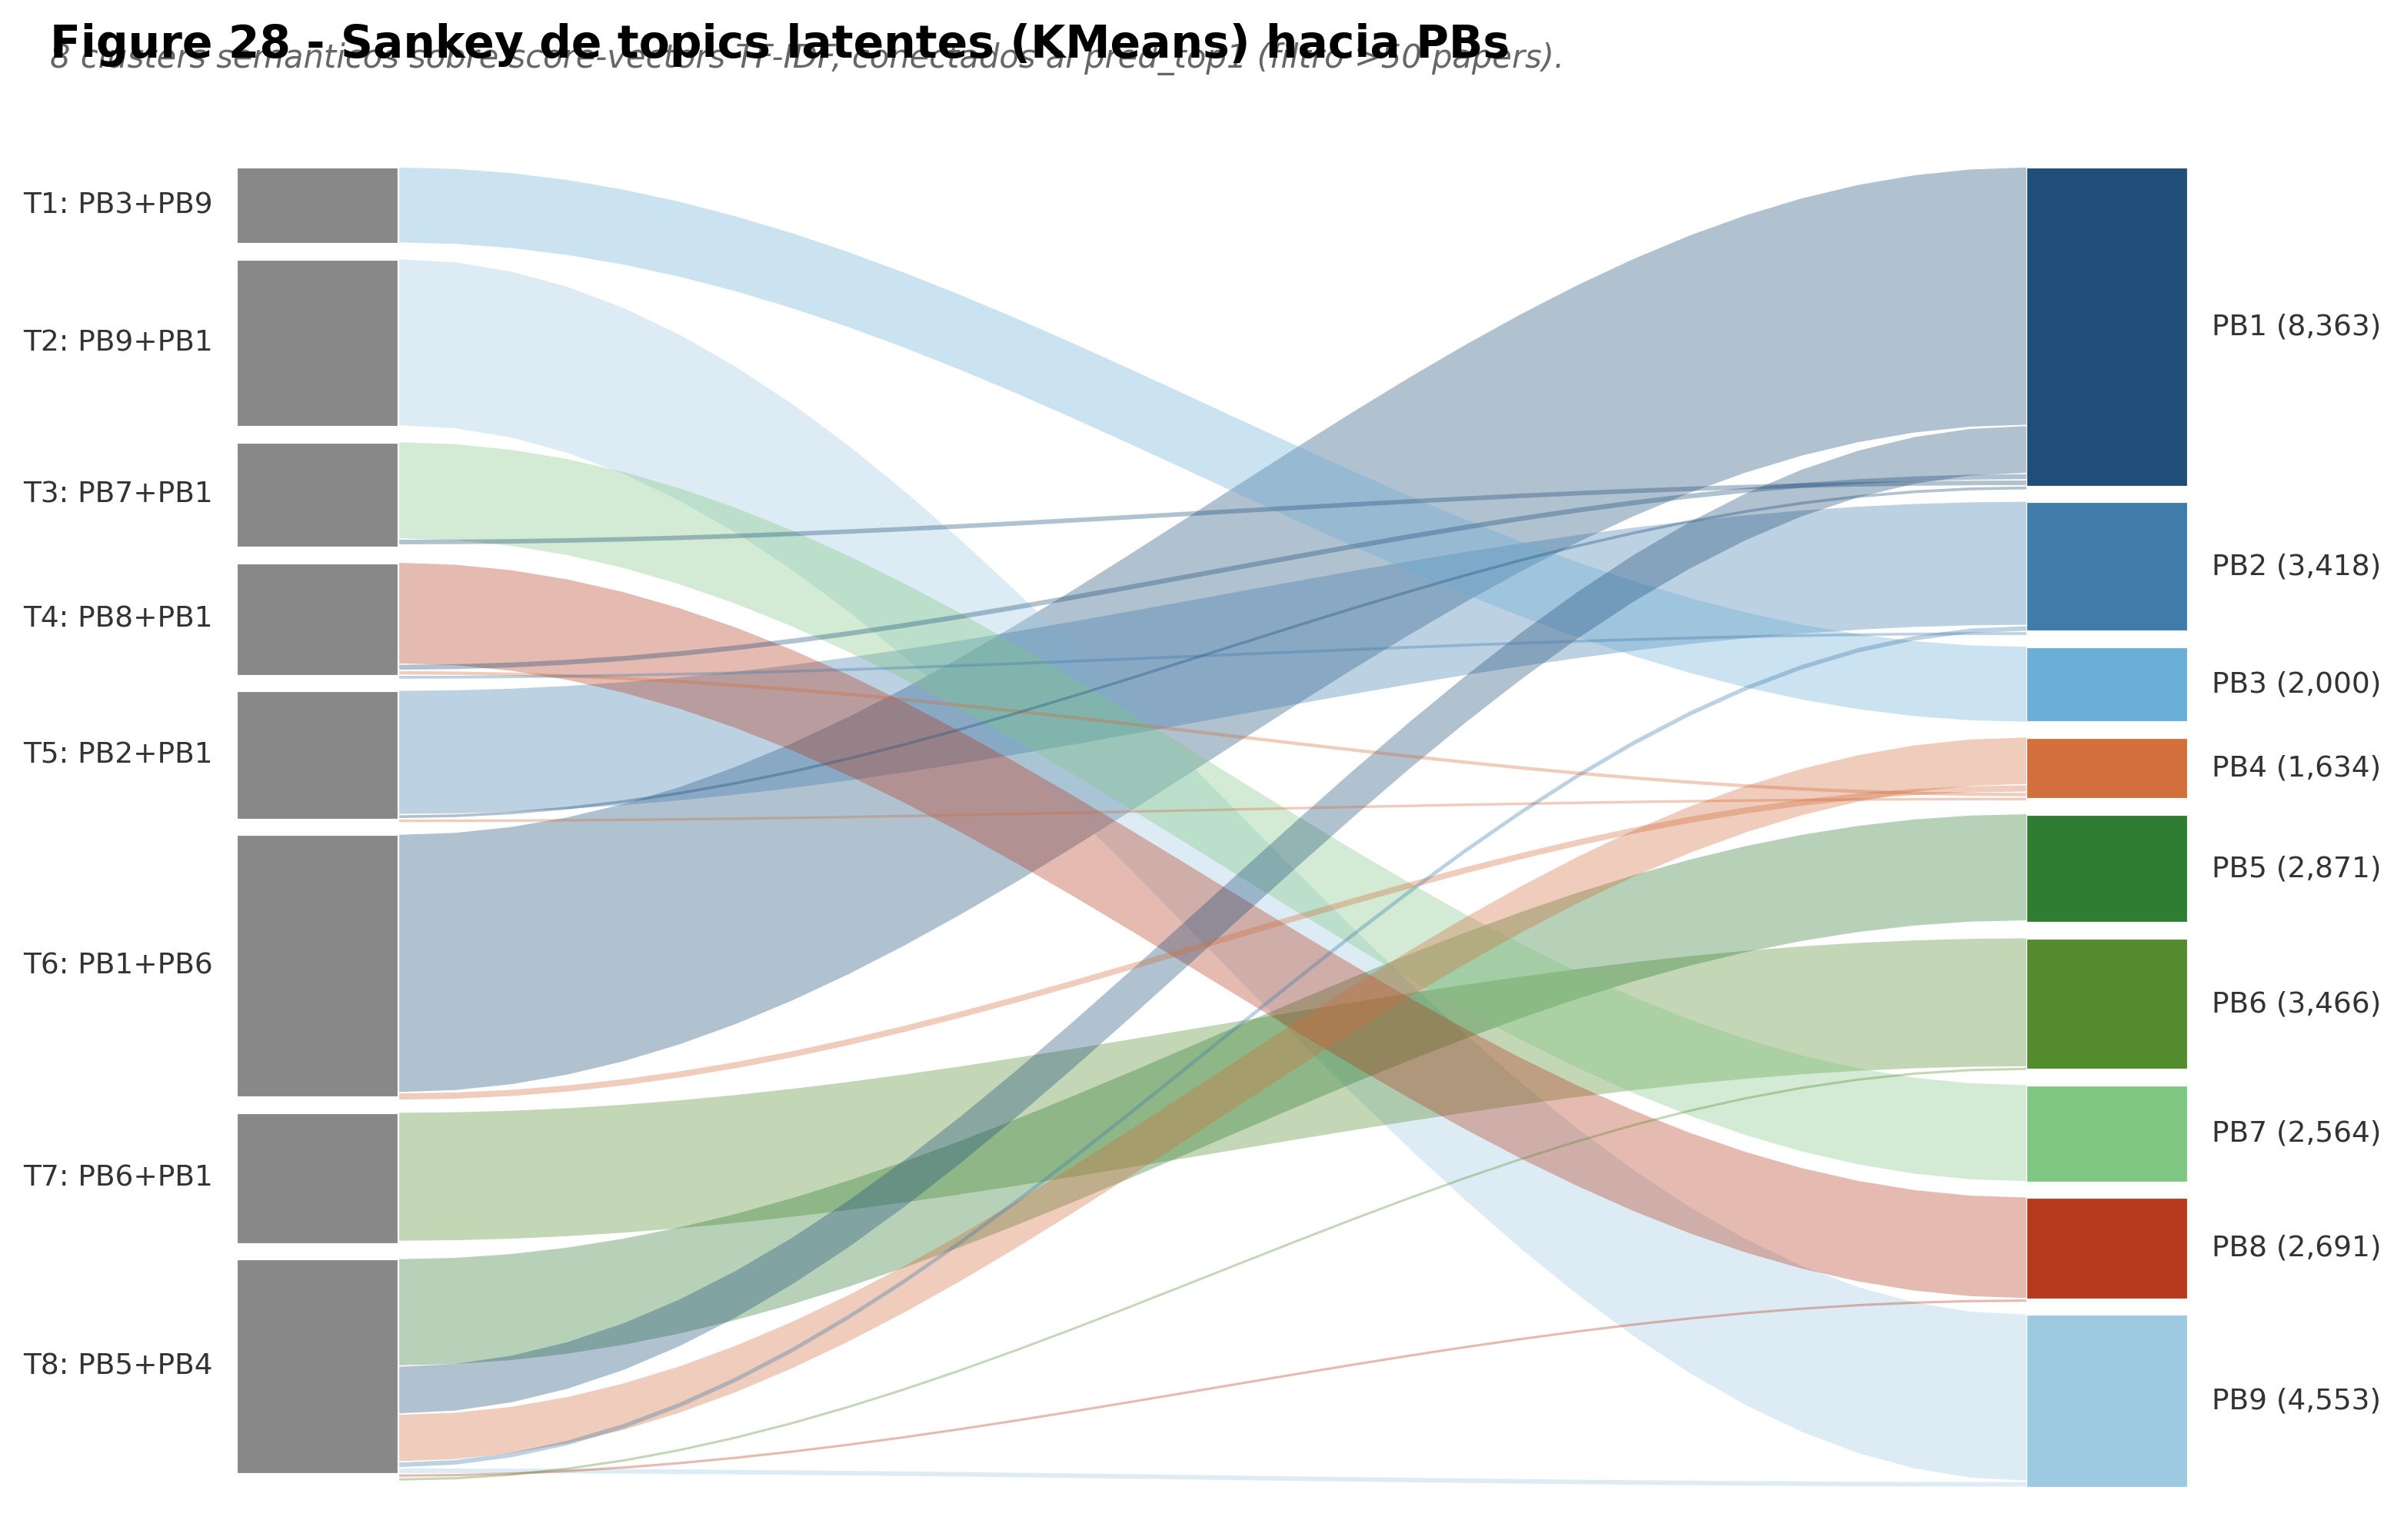
\includegraphics[width=0.85\linewidth]{figures/28_sankey_topics_pbs.png}
\caption{Sankey: 8 clusters semánticos $\to$ PBs. La consistencia del flujo (clusters dominados por un solo PB ramificándose limpiamente al PB correspondiente) confirma que la representación TF-IDF separa razonablemente las temáticas.}
\label{fig:sankey}
\end{figure}

% ============================================================
\section{Modelos de clasificación: evaluación crítica}\label{sec:modelos}

\subsection{Modelos evaluados}

Evaluamos seis enfoques con diseños deliberadamente distintos:

\begin{table}[h]
\centering\small
\begin{tabularx}{\linewidth}{l l X}
\toprule
\textbf{Modelo} & \textbf{Familia} & \textbf{Justificación de inclusión} \\
\midrule
\textsc{lexical} & keyword matching & Suelo de la tarea. Máxima interpretabilidad. \\
\textsc{tf-idf} & bag-of-words + cosine & Captura co-ocurrencias estadísticas, sin GPU. \\
\textsc{bert-base} \cite{devlin2019bert} & transformer general & Estándar de comparativa. \\
\textsc{roberta-base} \cite{liu2019roberta} & transformer general optimizado & Comparativa con BERT, mejoras documentadas en GLUE. \\
\textsc{scibert} \cite{beltagy2019scibert} & transformer en corpus científico & Test de la hipótesis ``vocabulario de dominio mejora''. \\
\textsc{specter} \cite{cohan2020specter} & transformer \emph{citation-aware} & Conceptualmente el correcto: entrenado para representar papers. \\
\bottomrule
\end{tabularx}
\caption{Los seis enfoques. Cada uno responde una pregunta distinta; no son redundantes.}
\end{table}

Para los transformers la representación de un documento es el \emph{mean-pooling} del \texttt{last\_hidden\_state} sobre la máscara de atención, normalizado L2. La asignación PB es por similitud coseno contra el embedding del documento PB de referencia.

\subsection{Panel de métricas}

Distinguimos siete familias de métricas, cada una respondiendo una pregunta operativa específica:

\begin{enumerate}
\item \textbf{Top-1 micro/macro F1}: $\mathbb{1}[\arg\max_i s_i = \text{gold}]$.
\item \textbf{Multilabel precision/recall/F1}: $|P \cap G|/|P|$, $|P \cap G|/|G|$.
\item \textbf{Jaccard samples}: $|P \cap G|/|P \cup G|$ promediado.
\item \textbf{Exact match}: $\mathbb{1}[P = G]$.
\item \textbf{Cobertura top-$k$ por nivel}: $g_1$, $g_2$, $g_3$ presentes en top-$k$.
\item \textbf{LRAP}: calidad del ranking, independiente de threshold.
\item \textbf{Ruido}: $|P \setminus G|/|P|$.
\end{enumerate}

\paragraph{Calibración del threshold.} Búsqueda en rejilla $\tau \in \{0{,}03, \ldots, 0{,}75\}$, $\delta \in \{0, \ldots, 0{,}20\}$ sobre el conjunto de validación. \textbf{Un hallazgo metodológico no trivial}: el grid inicial $\tau \geq 0{,}20$ es inapropiado para TF-IDF (cosines típicos $<0{,}15$ en espacios sparsos), provocando colapso multilabel a $\emptyset$. Re-calibrar con $\tau \geq 0{,}03$ sitúa a TF-IDF como modelo de referencia.

\subsection{Fórmulas compuestas}

Para componer las métricas anteriores en un único ranking definimos dos fórmulas:

\paragraph{Fórmula A: éxito ponderado.}
\begin{align}
\text{score}_A(d) = \;& 3{,}0 \cdot \mathbb{1}[\text{top1}=g_1] + 1{,}5 \cdot \mathbb{1}[g_1 \in \{\text{top1,top2}\}, \text{top1}\neq g_1] \nonumber \\
& + 1{,}0 \cdot \mathbb{1}[g_2 \in P] + 0{,}5 \cdot \mathbb{1}[g_3 \in P] - 0{,}25 \cdot |P \setminus G|
\end{align}

\paragraph{Fórmula B: MRR ponderado por nivel.}
\begin{equation}
\text{score}_B(d) = \sum_{i \in \{1,2,3\}} \frac{w_i \cdot \mathbb{1}[g_i \text{ existe}]}{\text{rank}_M(g_i)}, \qquad w_1=3, \; w_2=2, \; w_3=1
\end{equation}
donde $\text{rank}_M(g_i)$ es la posición de $g_i$ en el ranking descendente de scores del modelo $M$. Ambas fórmulas se normalizan por el máximo alcanzable.

\subsection{Resultados de validación}\label{sec:resval}

Validación contra 98 papers con 130 PBs anotados manualmente (\texttt{validacion\_real.csv}).

\begin{figure}[h]
\centering
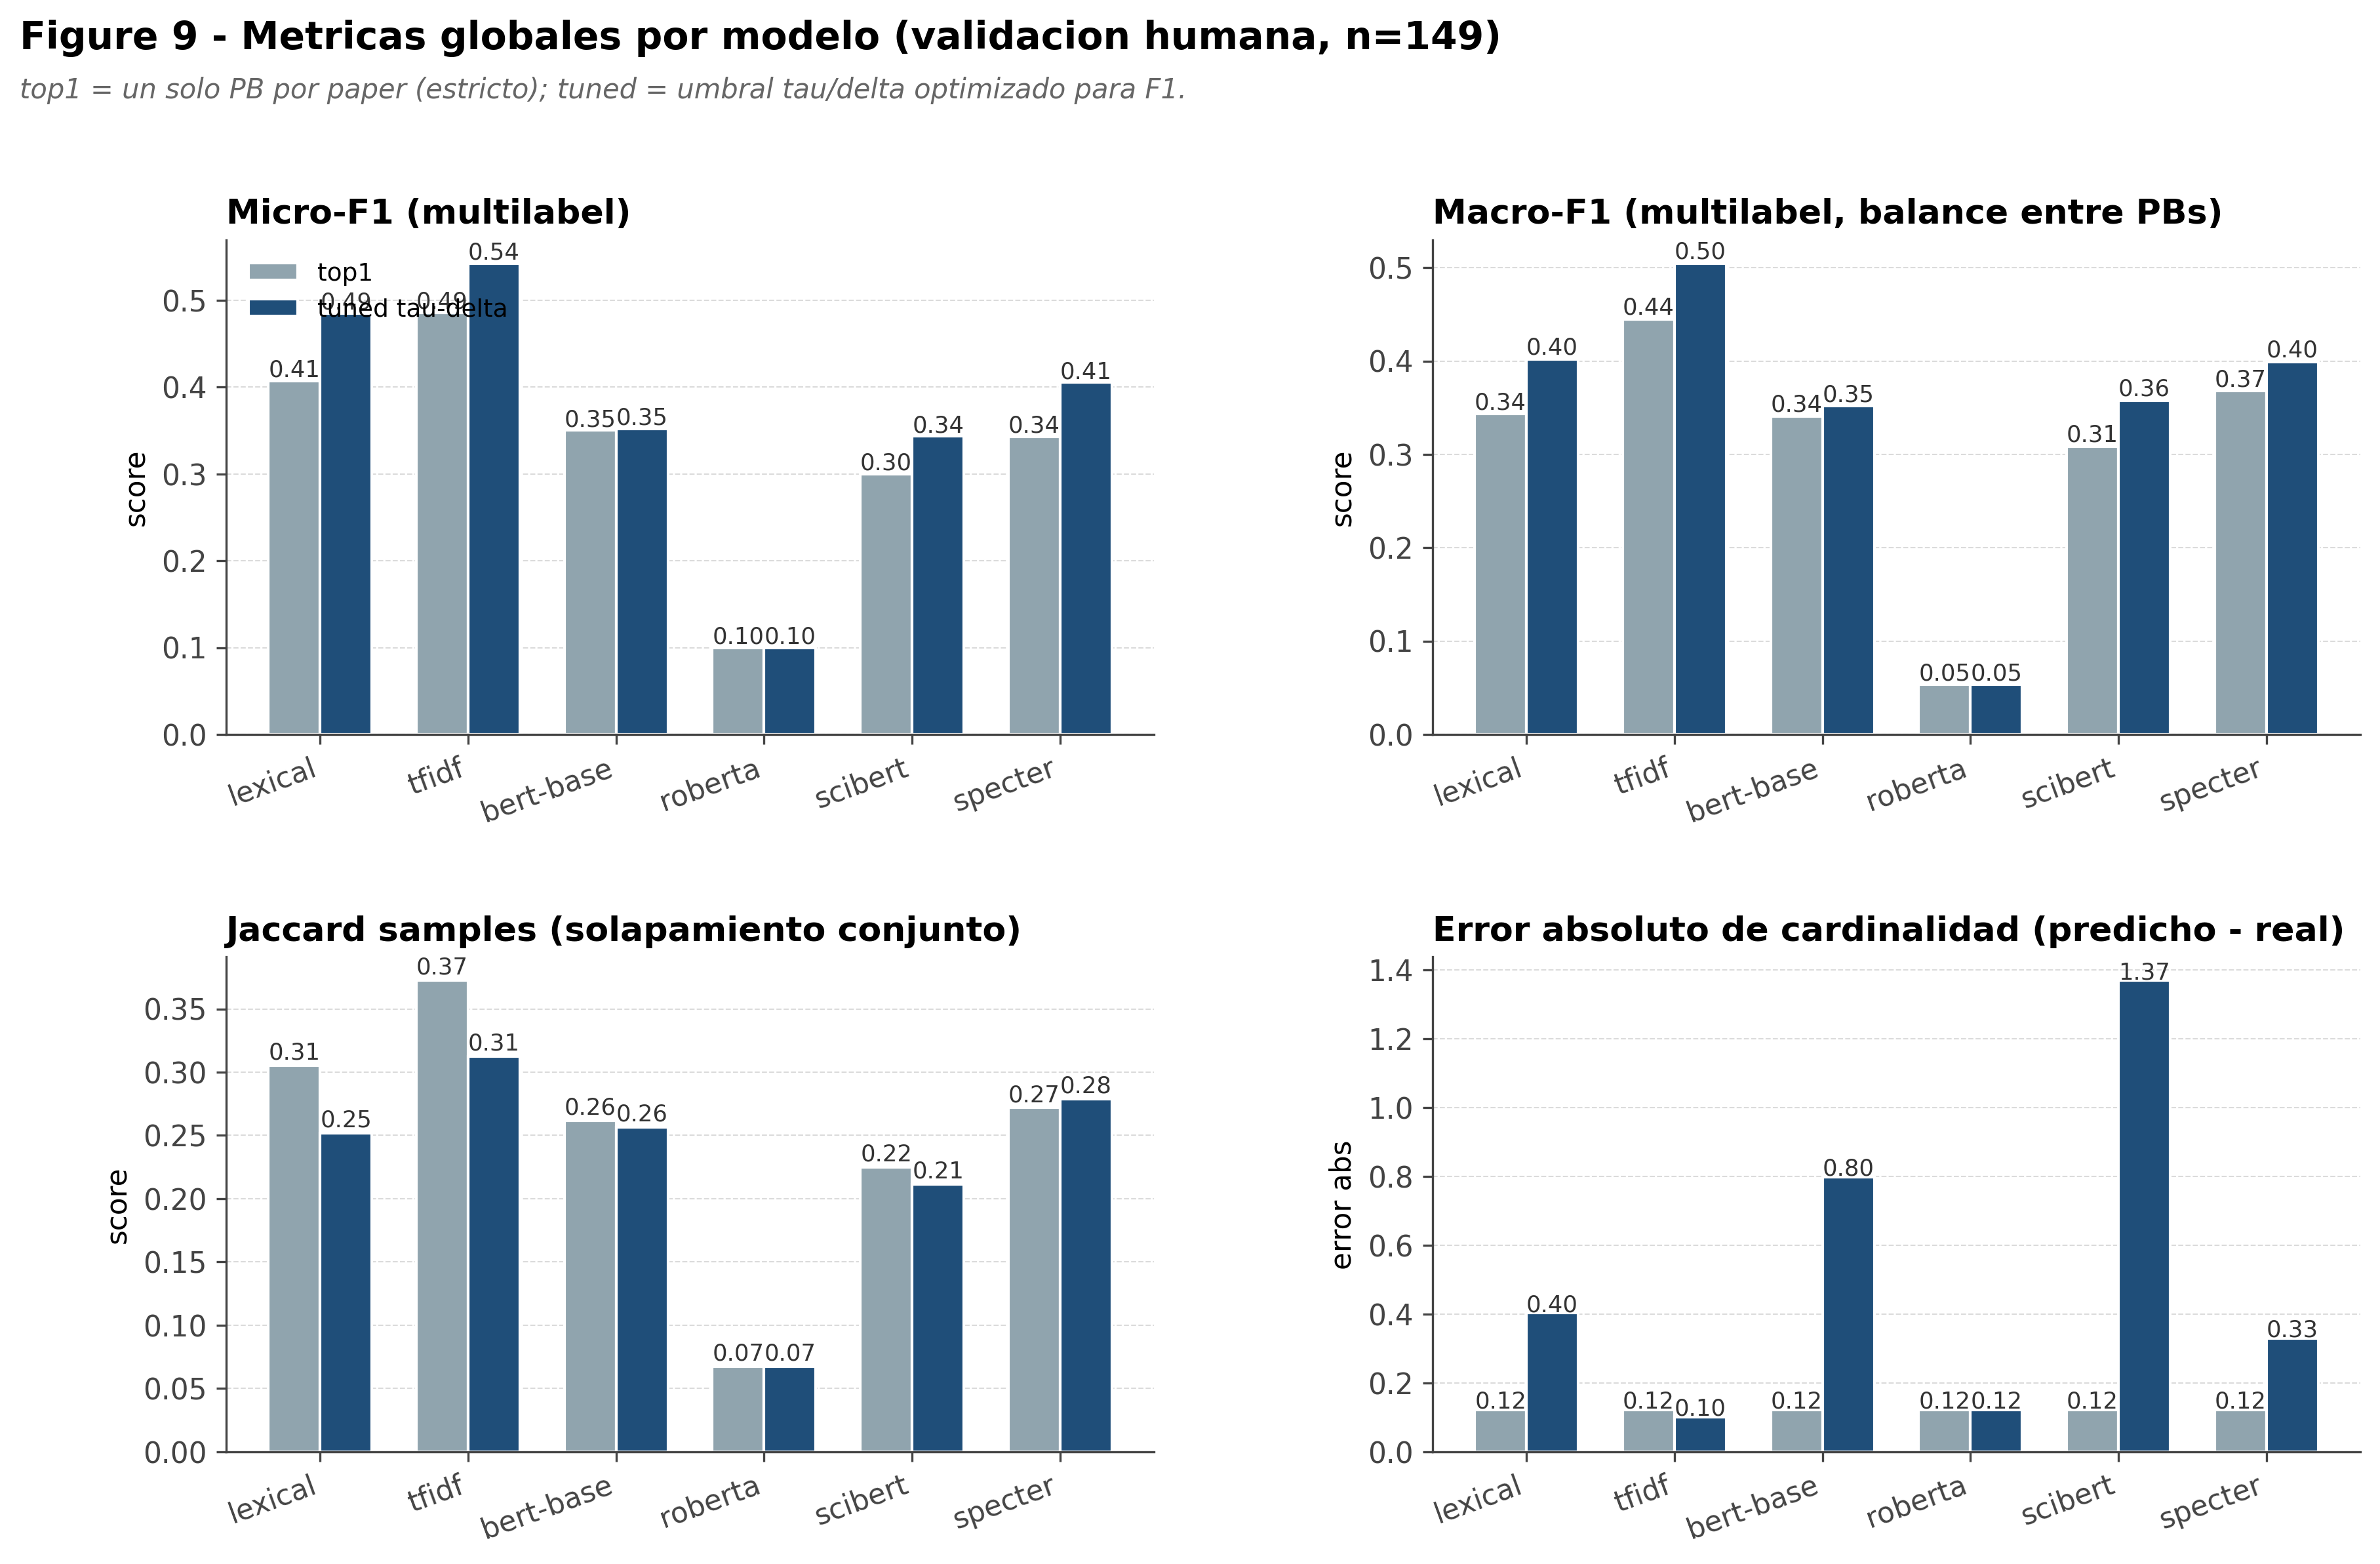
\includegraphics[width=\linewidth]{figures/09_metrics_overview.png}
\caption{Panel global de métricas: micro/macro F1, Jaccard, error absoluto de cardinalidad. Comparación top-1 vs threshold tuneado.}
\end{figure}

\begin{table}[h]
\centering\small
\begin{tabular}{l rrrrr | rrr}
\toprule
& \multicolumn{5}{c|}{\textbf{Multilabel}} & \multicolumn{3}{c}{\textbf{PB principal (1stpb)}} \\
\textbf{Modelo} & \textbf{Pred} & \textbf{Hit} & \textbf{P} & \textbf{R} & \textbf{F1} & \textbf{Top-1} & \textbf{Top-2} & \textbf{Top-3} \\
\midrule
\good{tf-idf} & 91 & 67 & 0{,}74 & \good{0{,}51} & \good{0{,}61} & \good{63\%} & \good{77\%} & \good{83\%} \\
lexical & 60 & 48 & \good{0{,}80} & 0{,}37 & 0{,}51 & 47\% & 55\% & 62\% \\
specter & 119 & 63 & 0{,}53 & 0{,}49 & 0{,}51 & 44\% & 67\% & 77\% \\
bert-base & 163 & 67 & 0{,}41 & 0{,}52 & 0{,}46 & 45\% & 64\% & 80\% \\
scibert & 218 & 80 & 0{,}37 & \good{0{,}62} & 0{,}46 & 38\% & 63\% & 81\% \\
roberta & 98 & 14 & 0{,}14 & 0{,}11 & 0{,}12 & 12\% & 25\% & 53\% \\
\bottomrule
\end{tabular}
\caption{Resultados de validación (n=98 docs, 130 PBs anotados). TF-IDF lidera en F1 multilabel y en cobertura top-$k$ del PB principal. Lexical alcanza la mejor precisión pero a costa de recall. SciBERT recall máximo pero con sobrecardinalidad.}
\label{tab:resultados}
\end{table}

\begin{figure}[h]
\centering
\begin{subfigure}{0.49\linewidth}
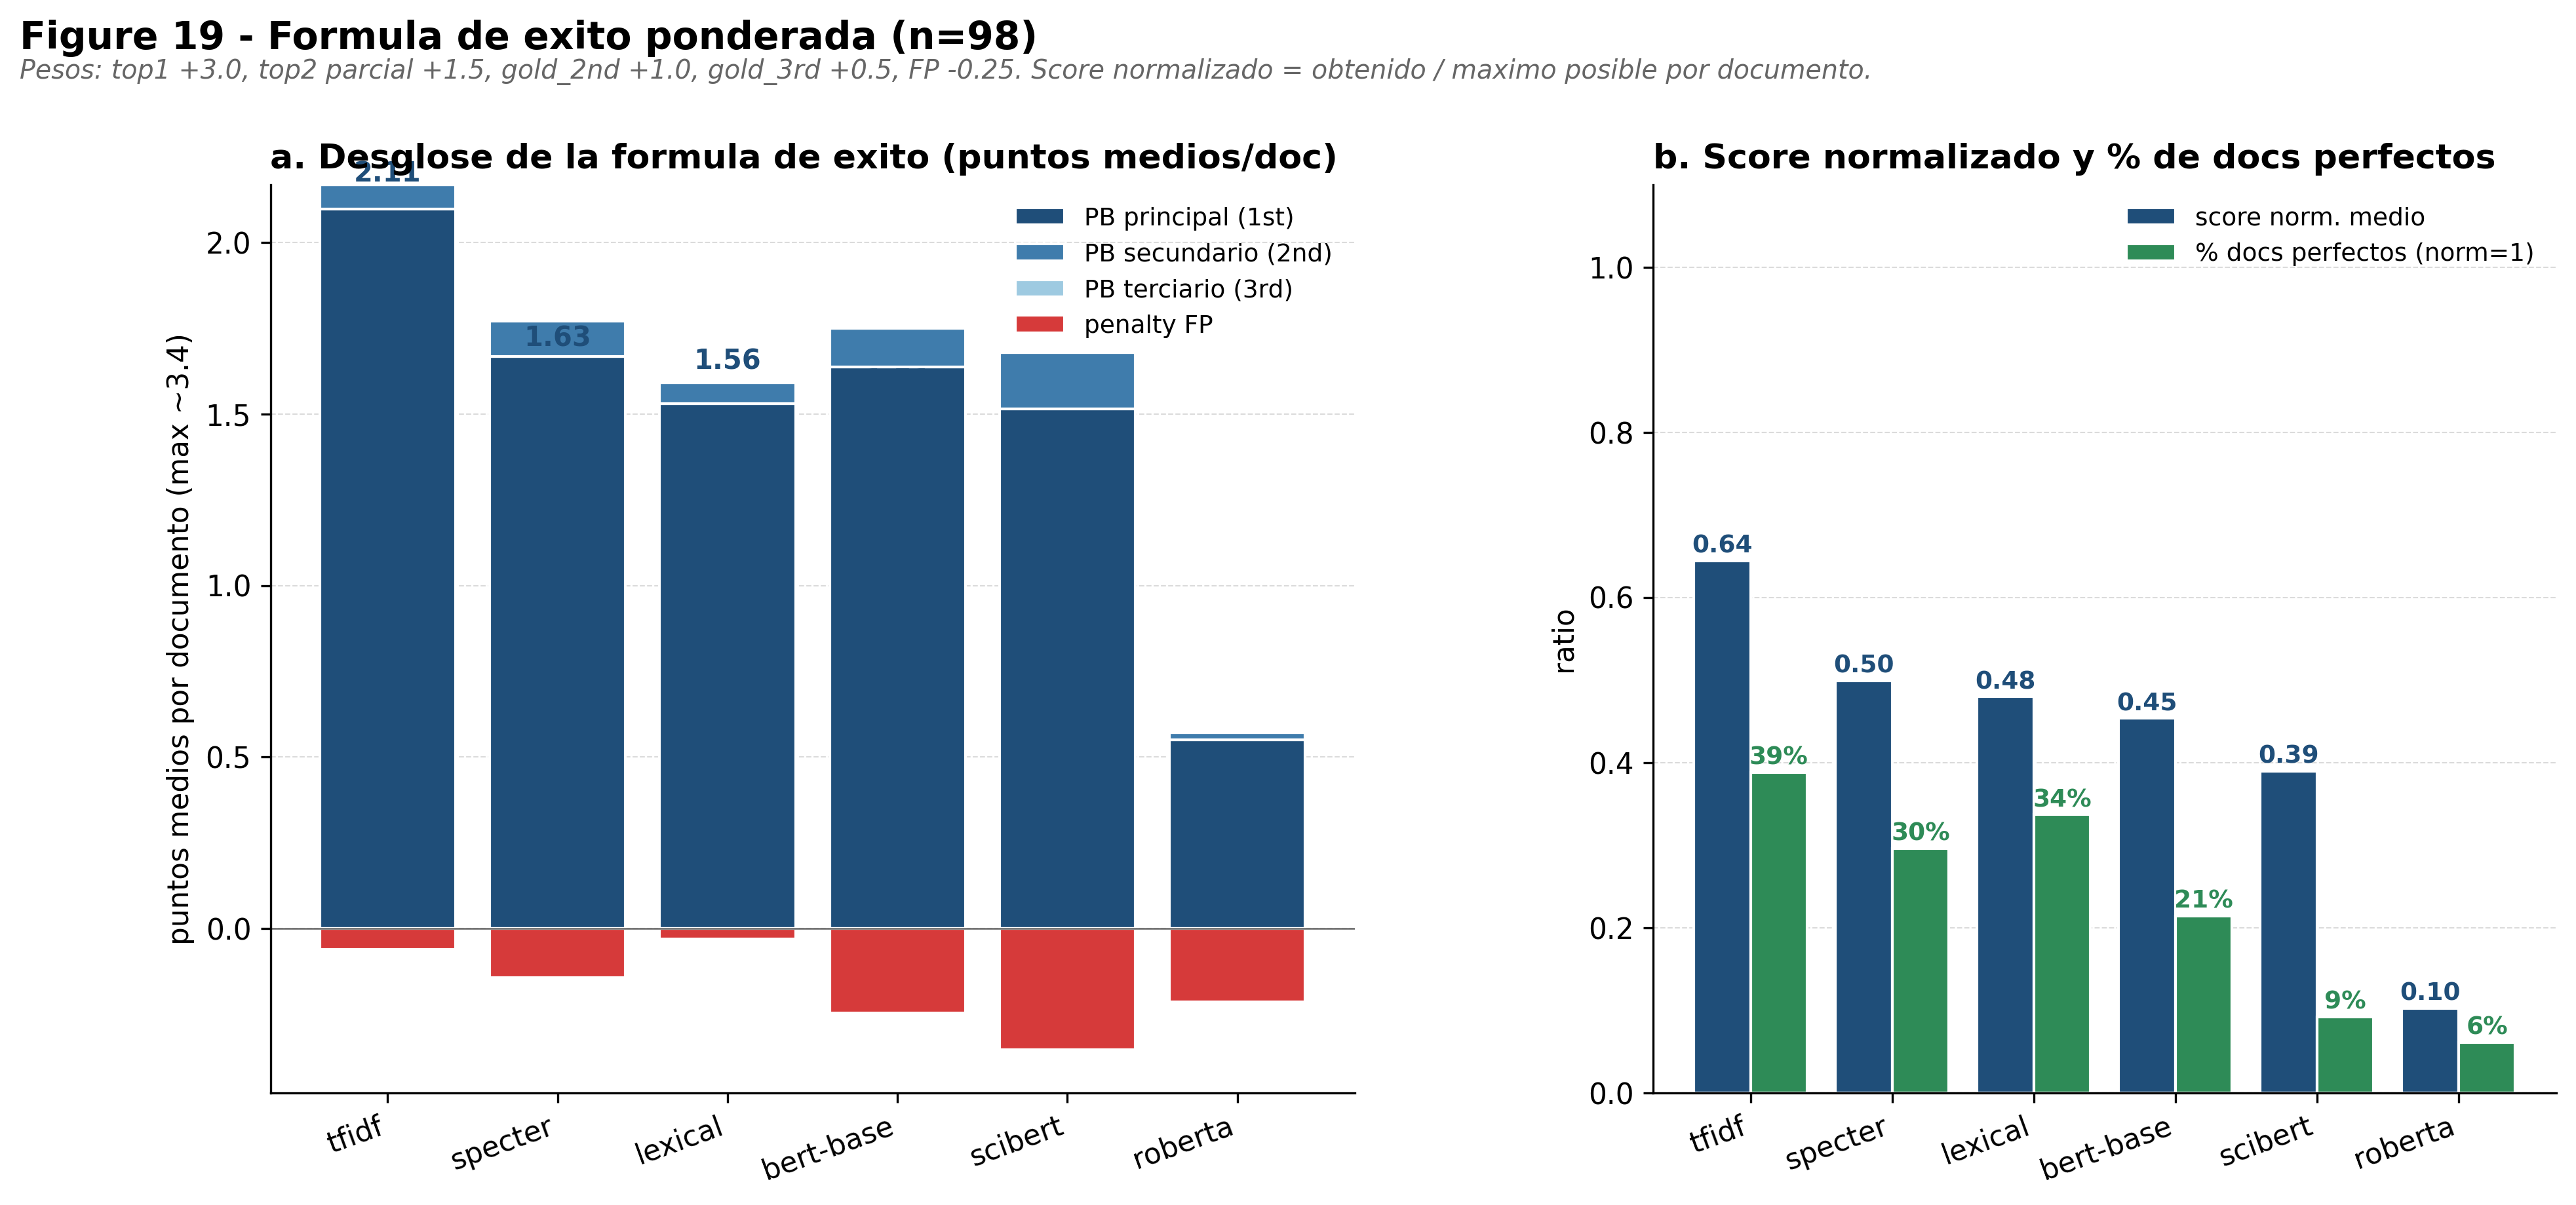
\includegraphics[width=\linewidth]{figures/19_success_formula.png}
\caption{Fórmula A: éxito ponderado.}
\end{subfigure}
\hfill
\begin{subfigure}{0.49\linewidth}
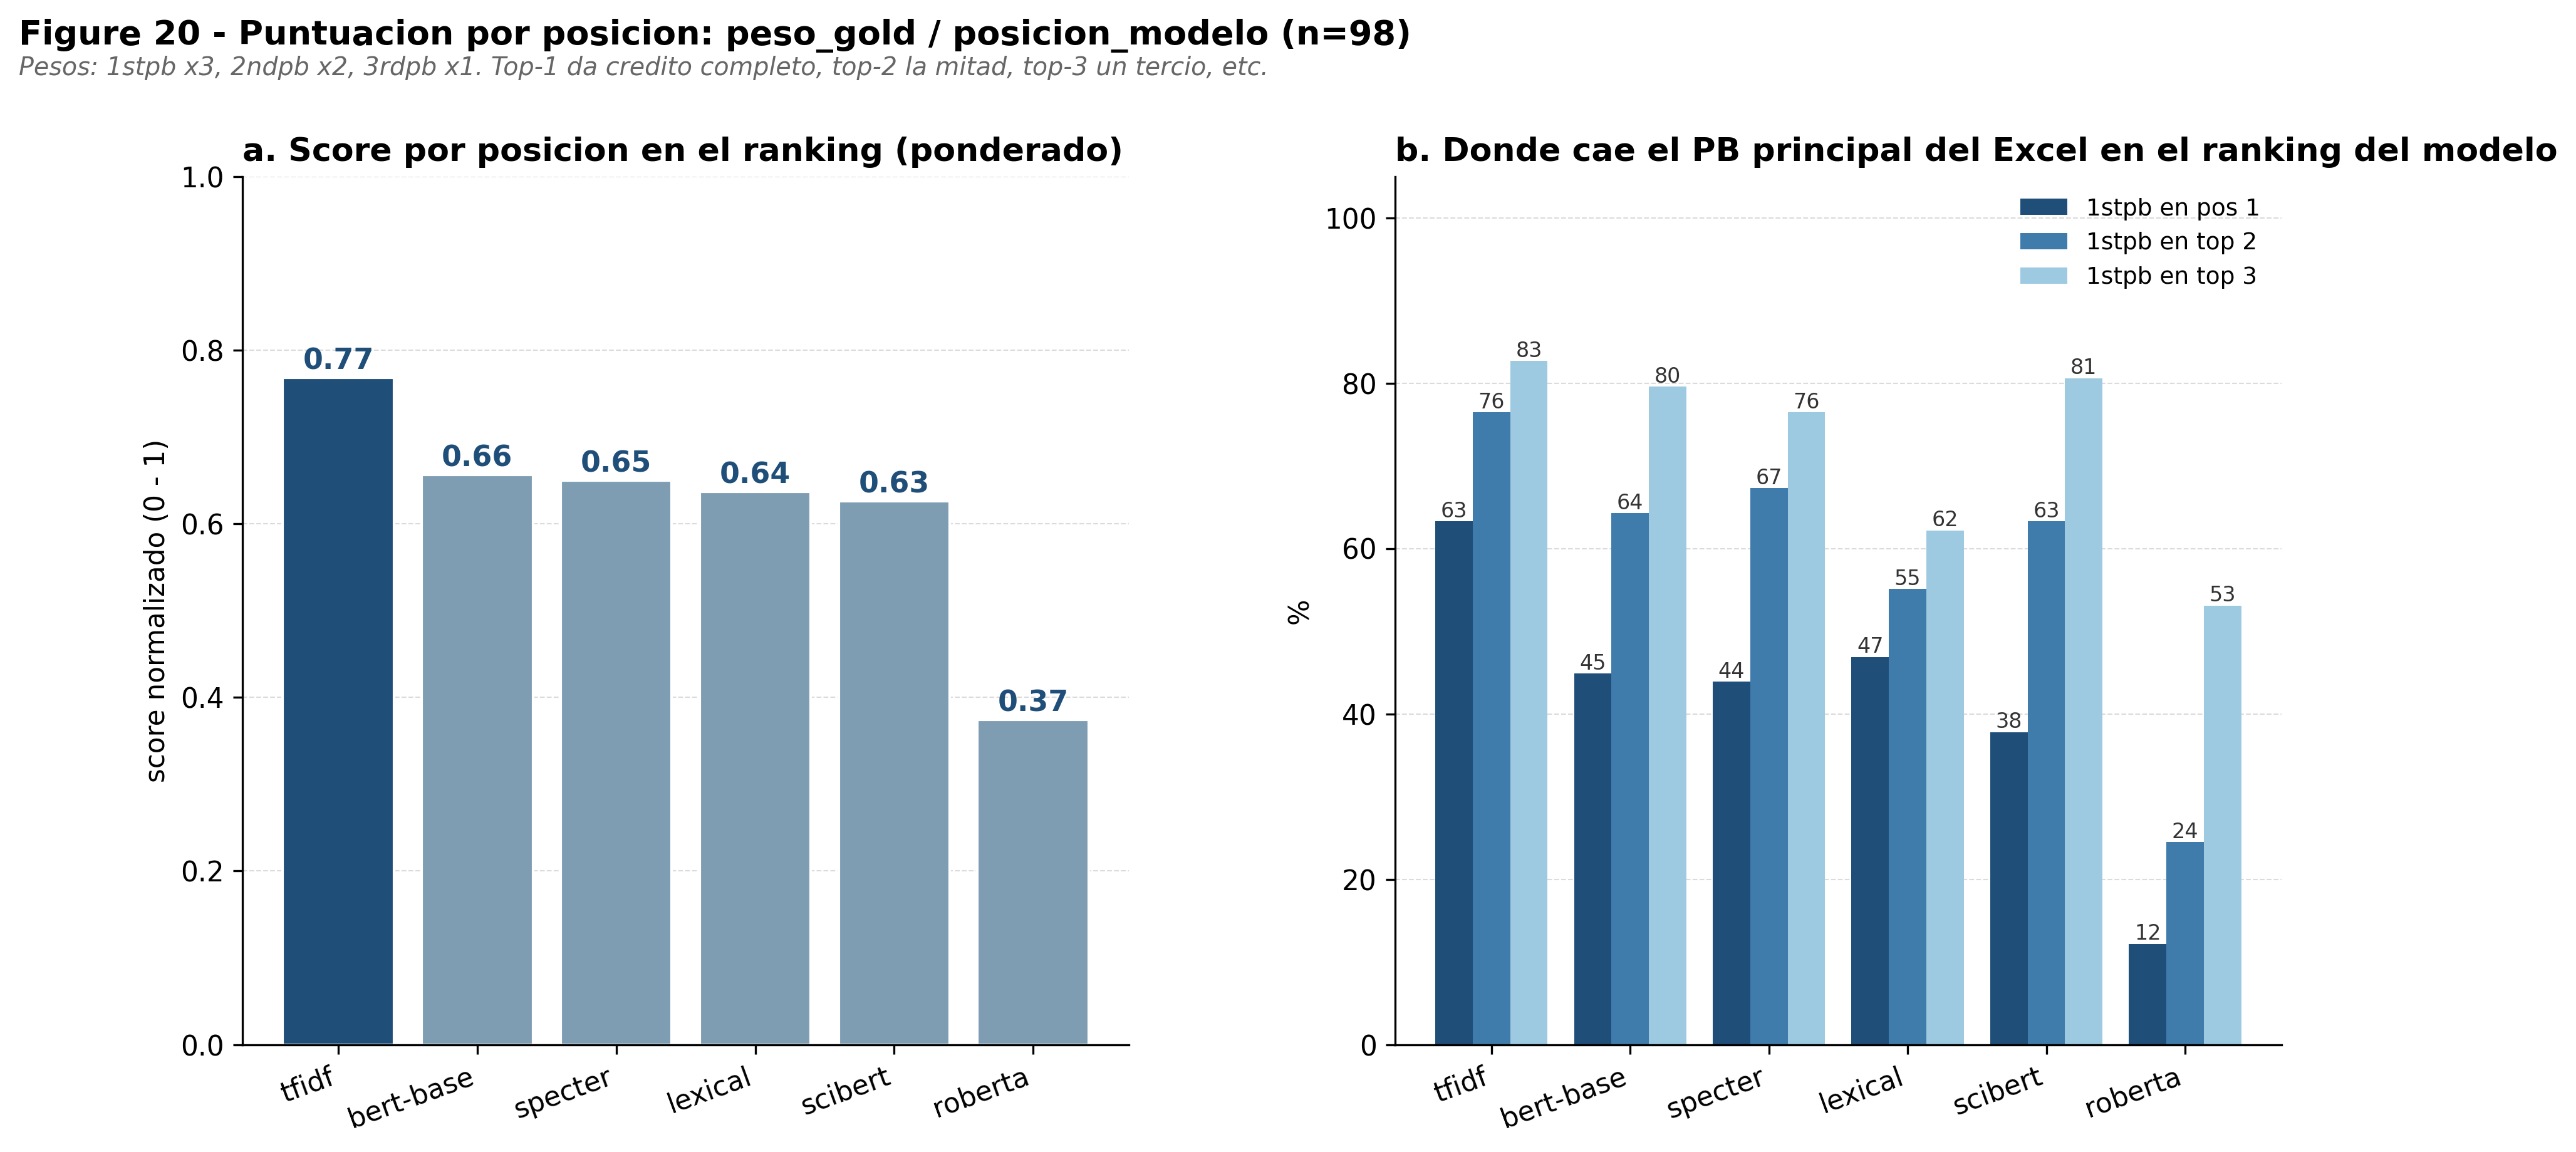
\includegraphics[width=\linewidth]{figures/20_rank_score.png}
\caption{Fórmula B: MRR ponderado.}
\end{subfigure}
\caption{Fórmulas compuestas. TF-IDF domina ambas (A=0{,}64; B=0{,}77).}
\end{figure}

\subsubsection{Análisis por PB: ¿qué modelo falla con cuál?}\label{sec:errores}

\begin{table}[h]
\centering\small
\begin{tabular}{l r|rrrrrr}
\toprule
\textbf{PB} & \textbf{Soporte} & \textbf{lex.} & \textbf{tf-idf} & \textbf{bert} & \textbf{rob.} & \textbf{scib.} & \textbf{spec.} \\
\midrule
\pb1 Climate & 38 & \good{0\%} & 13\% & 24\% & 74\% & 8\% & 47\% \\
\pb2 Ocean & 8 & \good{0\%} & \good{0\%} & 12\% & \good{0\%} & 12\% & 12\% \\
\pb3 Ozone & 8 & \good{12\%} & 38\% & 25\% & 50\% & 38\% & 38\% \\
\pb4 Biogeochem & 12 & 83\% & 33\% & 33\% & 42\% & 75\% & \good{8\%} \\
\pb5 Freshwater & 9 & 78\% & 22\% & 22\% & 100\% & 44\% & \good{11\%} \\
\pb6 Land-System & 6 & 83\% & 33\% & 17\% & \good{0\%} & \good{0\%} & 33\% \\
\pb7 Biosphere & 19 & 89\% & 32\% & 42\% & 53\% & \good{11\%} & 26\% \\
\pb8 Novel Ent. & 7 & 57\% & 43\% & \good{29\%} & 71\% & 57\% & 71\% \\
\pb9 Aerosol & 23 & 35\% & \good{4\%} & 17\% & 39\% & \good{4\%} & 9\% \\
\bottomrule
\end{tabular}
\caption{\% de papers donde el modelo pierde la PB anotada (no aparece en su top-3). En azul, el mínimo por fila. Ningún modelo es uniformemente bueno: la receta de ensemble por PB se deriva directamente de esta tabla.}
\label{tab:errores_pb}
\end{table}

\begin{figure}[h]
\centering
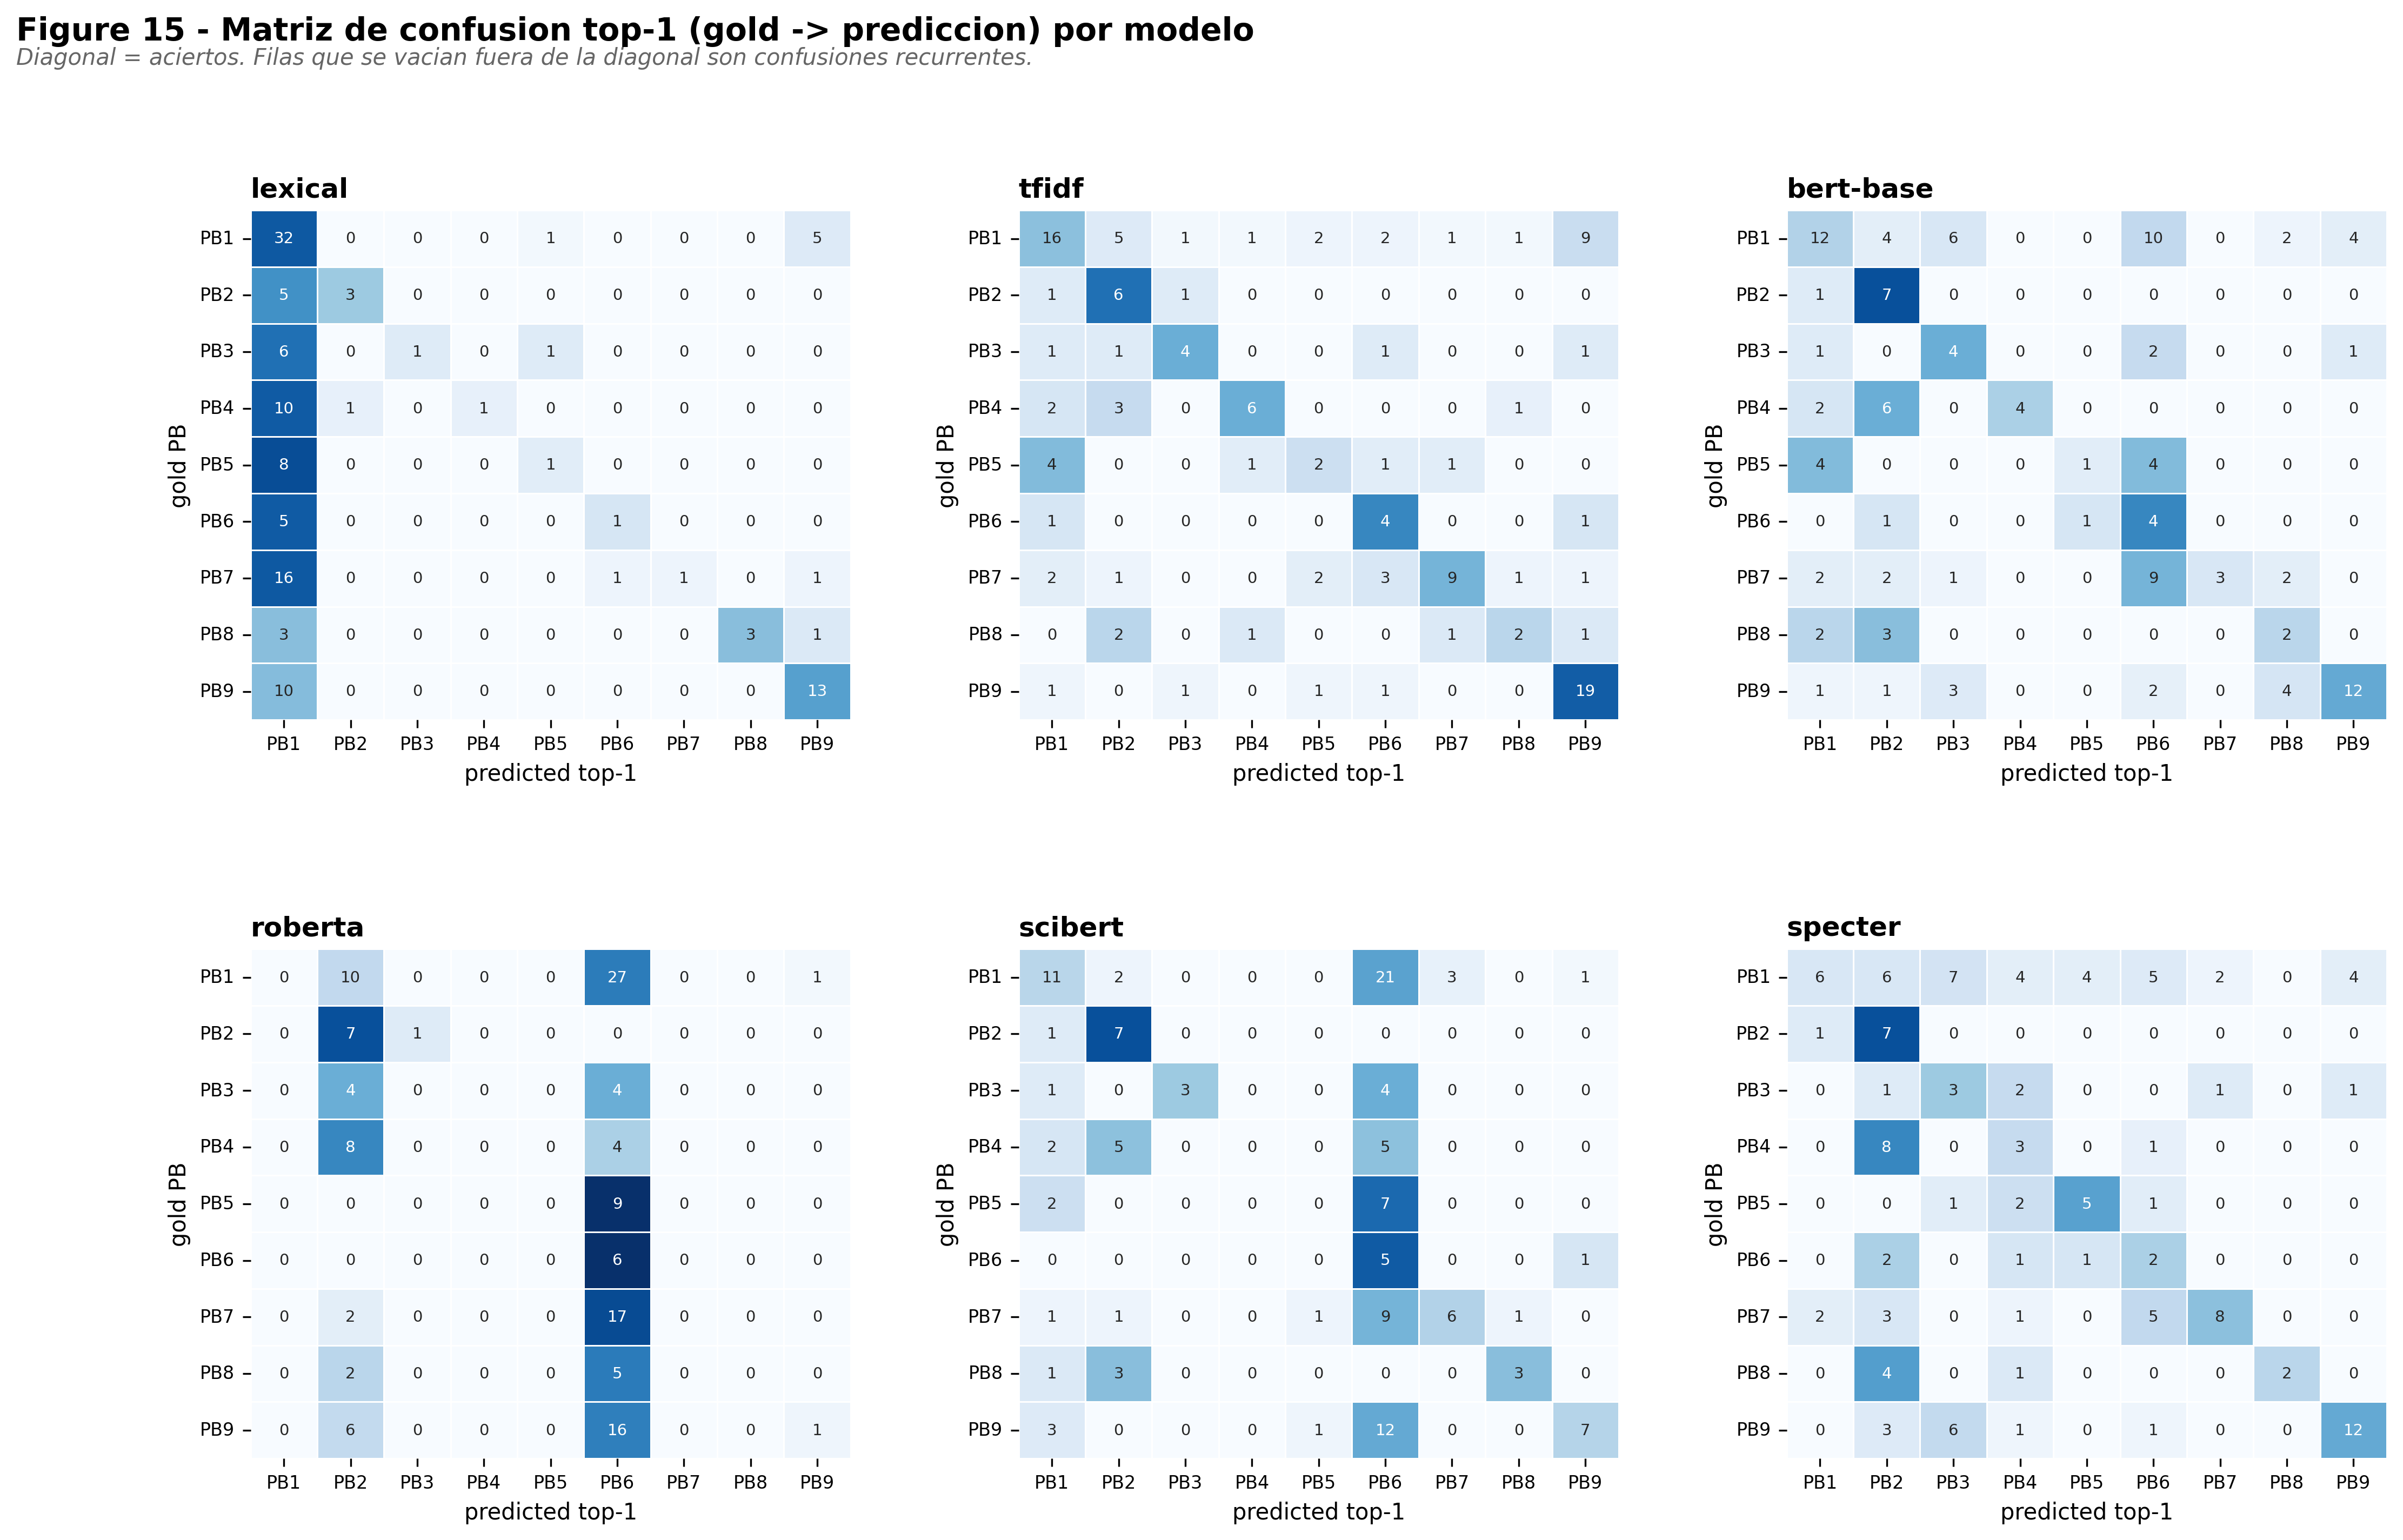
\includegraphics[width=\linewidth]{figures/15_confusion_per_model.png}
\caption{Matrices de confusión normalizadas por fila (gold $\to$ predicho top-1). Diagonal $=$ aciertos. Las confusiones de SPECTER son físicamente coherentes (\pb1$\leftrightarrow$\pb3, \pb4$\leftrightarrow$\pb2); las de BERT/SciBERT/RoBERTa convergen patológicamente a \pb6.}
\label{fig:conf}
\end{figure}

\subsubsection{Ruido (falsos positivos)}

\begin{table}[h]
\centering\small
\begin{tabular}{l rrrr}
\toprule
\textbf{Modelo} & \textbf{Pred} & \textbf{Correctos} & \textbf{Ruido} & \textbf{\% ruido} \\
\midrule
\good{lexical} & 60 & 48 & 12 & \good{20{,}0} \\
\good{tf-idf} & 91 & 67 & 24 & 26{,}4 \\
specter & 119 & 63 & 56 & 47{,}1 \\
bert-base & 163 & 67 & 96 & 58{,}9 \\
scibert & 218 & 80 & 138 & 63{,}3 \\
roberta & 98 & 14 & 84 & \bad{85{,}7} \\
\bottomrule
\end{tabular}
\caption{Ruido por modelo. Lexical produce 4 de cada 5 predicciones correctas; RoBERTa solo 1 de cada 7.}
\end{table}

% ============================================================
\section{Discusión crítica}\label{sec:discusion}

\subsection{¿Por qué TF-IDF supera a transformers no fine-tuneados?}

Tres factores se combinan:

\paragraph{(i) Los transformers no están fine-tuneados.} Mean-pooling sobre \texttt{last\_hidden\_state} es la peor configuración para usar BERT en clasificación temática. Equivale a usar el modelo como extractor de features sin proyección supervisada. Un \textbf{fine-tune contrastivo de SPECTER} sobre las 138 anotaciones humanas (loss tipo NTXent \cite{chen2020simple}) debería superar a TF-IDF; es el siguiente paso técnico.

\paragraph{(ii) La tarea tiene mucha señal léxica.} Los abstracts académicos contienen \emph{explícitamente} terminología PB. TF-IDF aprovecha esto. No es magia: es que el problema, parcialmente, es de coincidencia léxica calibrada.

\paragraph{(iii) Los documentos PB de referencia son listas de keywords.} TF-IDF compara dos representaciones de la misma naturaleza (bag-of-words técnico). Un documento PB redactado en prosa fluida desplazaría la ventaja hacia SPECTER.

\paragraph{Conclusión.} TF-IDF no es ``mejor'' en abstracto, es \emph{mejor en este setup}. Es un resultado válido y reportable, pero no extrapolable.

\subsection{Patrones patológicos}

\begin{itemize}
\item \textbf{Atractor a \pb6 en transformers genéricos.} BERT, RoBERTa y SciBERT arrastran sistemáticamente hacia \pb6. RoBERTa confunde \pb1$\to$\pb6 en 27 papers, \pb7$\to$\pb6 en 17, \pb9$\to$\pb6 en 16. La hipótesis razonable: el vocabulario ``land'', ``surface'', ``system'' tiene una representación atractiva en el embedding mean-pooled, no contrarrestada por fine-tune supervisado.
\item \textbf{Colapso de RoBERTa.} Cosines $>0{,}99$ entre clases para muchos documentos. La distribución de scores es plana; el modelo es inservible sin proyección adaptada.
\item \textbf{Sobre-cardinalidad de SciBERT.} 218 PBs predichos sobre 130 reales (1{,}68$\times$). Su recall alto (0{,}62) se paga con 138 falsos positivos.
\end{itemize}

Las confusiones de SPECTER son distintas: \pb1$\leftrightarrow$\pb3, \pb4$\leftrightarrow$\pb2. Son errores intrafamilia, físicamente coherentes. Los de BERT/SciBERT son arbitrarios.

\subsection{Limitaciones metodológicas}

\begin{enumerate}
\item \textbf{Tamaño muestral (n=98, soportes por PB hasta 6).} Para soporte $s$ y proporción observada $\hat{p}$, el intervalo de confianza binomial al 95\,\% es $\hat{p} \pm 1{,}96\sqrt{\hat{p}(1-\hat{p})/s}$. Para $s=6$ y $\hat{p}=0$, el IC superior es $\approx 0{,}39$. Cualquier ranking por-PB es ruidoso.
\item \textbf{Ausencia de test independiente.} La calibración $\tau, \delta$ se hizo sobre la muestra de validación. Es \emph{data leakage}. Para publicación, $k$-fold sobre las anotaciones es obligatorio.
\item \textbf{Anotador único.} Sin inter-annotator agreement no conocemos el techo de la tarea. Si dos humanos coincidieran solo el 70\,\%, ningún modelo puede aspirar a más.
\item \textbf{Heterogeneidad temporal.} SPECTER vio papers hasta 2020. Terminología emergente puede degradar la representación en abstracts 2023--2024.
\item \textbf{Sesgo de selección del ground truth.} Los 138 papers se anotaron por procedimiento no documentado en este AED. Si están sesgados temáticamente, las métricas no son representativas del comportamiento sobre los 31\,560 documentos.
\end{enumerate}

\subsection{Lo que NO se debe afirmar sin asterisco}

\begin{itemize}
\item ``SPECTER es peor que TF-IDF'' $\to$ \emph{en este setup zero-shot}. Con fine-tune contrastivo plausiblemente se invierte.
\item ``\pb8 es solo el 2\,\% del corpus UPV'' $\to$ esa cifra viene de un modelo cuyo F1 en \pb8 es $\sim 0{,}15$. Una fracción no medida de \pb8 reales puede estar mal etiquetada.
\item ``El modelo acierta el 63\,\%'' $\to$ sobre 98 docs con distribución desbalanceada, sin test independiente, anotador único.
\end{itemize}

% ============================================================
\section{Recomendación operativa}\label{sec:recomendacion}

\subsection{Modelo único para producción}

\begin{itemize}
\item \textbf{Tema principal de un paper}: TF-IDF top-2. 77\,\% acierto del \texttt{1stpb}.
\item \textbf{Multilabel realista}: TF-IDF, $\tau{=}0{,}03$, $\delta{=}0{,}08$. F1$=0{,}61$.
\item \textbf{Filtro de alta precisión (auto-anotación sin revisión)}: lexical. P$=0{,}80$.
\item \textbf{Exploración interdisciplinar}: SPECTER. Sus confusiones son borderline coherentes.
\item \textbf{No usar}: RoBERTa (colapsa); BERT/SciBERT sin fine-tune (atractor \pb6).
\end{itemize}

\subsection{Ensemble por PB}

De la Tabla~\ref{tab:errores_pb} se deriva una receta de ensemble \emph{por clase}:

\begin{table}[h]
\centering\small
\begin{tabular}{l l r}
\toprule
\textbf{PB} & \textbf{Modelo recomendado} & \textbf{\% pérdida} \\
\midrule
\pb1, \pb2, \pb3 & \textsc{lexical} & 0--12 \\
\pb4, \pb5 & \textsc{specter} & 8--11 \\
\pb6, \pb7 & \textsc{scibert} & 0--11 \\
\pb8 & \textsc{bert-base} & 29 \\
\pb9 & \textsc{tf-idf} \emph{o} \textsc{scibert} & 4 \\
\bottomrule
\end{tabular}
\caption{Ensemble por PB. Pérdida agregada estimada: $\sim 8\,\%$ (media ponderada por soporte), frente al $\sim 20\,\%$ del mejor modelo individual.}
\end{table}

\subsection{Asignación final del corpus}

Producimos un fichero \texttt{data/corpus/pb\_assignments\_top3.csv} con tres PBs por paper (top-3 ranking de TF-IDF) más scores, márgenes y nivel de confianza. La distribución de confianza es: alta 18\,\%, media 22\,\%, baja 60\,\%. La fracción de baja confianza es alta: en producción debe enseñarse al usuario los tres top-3, no solo el primero.

% ============================================================
\section{Trabajo futuro y siguiente paso crítico}

El siguiente paso técnico evidente es \textbf{fine-tunear SPECTER} sobre las 138 anotaciones humanas con \emph{contrastive learning}:

\begin{enumerate}
\item Construir pares positivos (abstract, documento PB anotado) y negativos (abstract, documento PB no anotado).
\item Loss tipo triplet o NTXent sobre la cabeza de pooling.
\item Cross-validation 5-fold para honestidad metodológica.
\item Re-evaluar con el mismo panel de métricas.
\end{enumerate}

La predicción razonable es que SPECTER-tuned superaría a TF-IDF, especialmente en \pb4, \pb5 y \pb7. Sin ese experimento, el ranking actual es el real.

\paragraph{Otros trabajos pendientes:} (i) \emph{contribution type} con LLM (monitoring / mitigation / pressure / methodology) sobre los 31\,560 abstracts; (ii) anotación humana expandida (n $\geq$ 400) con doble anotador para inter-annotator agreement; (iii) análisis por área Scopus/OpenAlex y bipartito disciplinas$\to$PBs; (iv) dashboard interactivo con filtros temporales y por PB.

% ============================================================
\section{Conclusiones}

\begin{enumerate}
\item La firma PB de la UPV es \textbf{cualitativamente robusta}: \pb1, \pb6, \pb2 dominantes; \pb8 marginal. Robusta a la elección del modelo (excluida RoBERTa) y al tamaño de muestra.
\item TF-IDF con threshold calibrado es el mejor modelo de los seis evaluados en \emph{zero-shot}: F1 multilabel $=0{,}61$, score MRR ponderado $=0{,}77$, 77\,\% top-2 acierto del PB principal.
\item Los transformers genéricos sin fine-tune muestran patologías sistemáticas (atractor a \pb6, colapso de RoBERTa) que invalidan su uso en producción.
\item SPECTER es el único transformer competitivo con errores físicamente coherentes; es la apuesta para fine-tune supervisado.
\item Las interacciones \pb3$\leftrightarrow$\pb9, \pb4$\leftrightarrow$\pb5, \pb6$\leftrightarrow$\pb7 emergen en todos los modelos competitivos: control de calidad implícito del etiquetado.
\item Ningún modelo es uniformemente bueno por PB. Un ensemble por clase reduce la pérdida agregada al $\sim 8\,\%$.
\item Las limitaciones (n pequeño, leak de threshold, anotador único) acotan las cifras absolutas, pero no las conclusiones cualitativas.
\end{enumerate}

% ============================================================
\begin{thebibliography}{99}\small

\bibitem{steffen2015planetary} Steffen, W., et al.\ (2015). Planetary boundaries: Guiding human development on a changing planet. \emph{Science}, 347(6223).

\bibitem{rockstrom2009safe} Rockström, J., et al.\ (2009). A safe operating space for humanity. \emph{Nature}, 461.

\bibitem{persson2022outside} Persson, L., et al.\ (2022). Outside the safe operating space of the planetary boundary for novel entities. \emph{Environmental Science \& Technology}, 56(3).

\bibitem{larosa2023climate} Larosa, F., et al.\ (2023). Mapping the landscape of climate services with LLMs. \emph{Environmental Research Letters}.

\bibitem{upv_ods_2024} Grupo UPV-ODS (2024). Análisis de la producción científica UPV en el marco ODS. Informe técnico, UPV.

\bibitem{devlin2019bert} Devlin, J., et al.\ (2019). BERT: Pre-training of Deep Bidirectional Transformers. \emph{NAACL-HLT}.

\bibitem{liu2019roberta} Liu, Y., et al.\ (2019). RoBERTa: A Robustly Optimized BERT Pretraining Approach. \emph{arXiv:1907.11692}.

\bibitem{beltagy2019scibert} Beltagy, I., Lo, K., Cohan, A.\ (2019). SciBERT: A Pretrained Language Model for Scientific Text. \emph{EMNLP}.

\bibitem{cohan2020specter} Cohan, A., et al.\ (2020). SPECTER: Document-level Representation Learning using Citation-informed Transformers. \emph{ACL}.

\bibitem{chen2020simple} Chen, T., et al.\ (2020). A Simple Framework for Contrastive Learning of Visual Representations. \emph{ICML}.

\bibitem{mcinnes2018umap} McInnes, L., Healy, J., Melville, J.\ (2018). UMAP: Uniform Manifold Approximation and Projection. \emph{arXiv:1802.03426}.

\end{thebibliography}

\appendix
\section{Reproducibilidad}

Todo el pipeline es reproducible mediante los siguientes comandos:

\begin{verbatim}
# Inferencia sobre el corpus completo con limpieza
python nlp/bert_finetuning/pb_backbones_benchmark.py \
  --corpus data/corpus/master_corpus_mixto_clean_enriched.csv \
  --traceability data/corpus/master_corpus_mixto_traceability.csv \
  --validation nlp/llm/outputs/ground_truth/validacion_real.csv \
  --models "allenai/specter,allenai/scibert_scivocab_uncased,
            bert-base-uncased,roberta-base" \
  --clean-text --batch-size 64 \
  --tau-grid 0.03,0.05,0.07,0.09,0.12,0.15,0.18,0.20,0.25,
             0.30,0.35,0.40,0.45,0.50,0.55,0.60,0.65,0.70,0.75 \
  --delta-grid 0.00,0.01,0.02,0.04,0.06,0.08,0.10,0.12,0.15,0.20 \
  --out-dir nlp/bert_finetuning/outputs_full

# Figuras AED principales
python scripts/aed_master.py
python scripts/aed_extended.py
python scripts/aed_metrics.py
python scripts/aed_validation.py
python scripts/aed_validation_primary.py
python scripts/aed_success_formula.py
python scripts/aed_rank_score.py

# Asignación PB final
python scripts/assign_pb_final.py
\end{verbatim}

\section{Inventario de figuras y datos}

29 figuras totales en \texttt{docs/eda/aed/figures/}, datos plot-ready de cada figura en \texttt{docs/eda/aed/data\_json/}. Tablas reutilizables en \texttt{docs/eda/aed/tables/}. Predicciones de los 6 modelos sobre los 31\,560 abstracts en \texttt{nlp/bert\_finetuning/outputs\_full/}.

\end{document}
